% chktex-file 29
% chktex-file 13
\documentclass{report}
\usepackage{setspace}
\usepackage[a4paper, total={7in, 9in}]{geometry}
\usepackage[fleqn]{amsmath}
\usepackage{empheq}
\usepackage{amssymb}
\usepackage{gensymb}
\usepackage[fleqn]{cases}
\usepackage{multicol}
\usepackage{color}
\usepackage{stix}
\usepackage{chngcntr}
\usepackage{tikz}
\usepackage{enumitem}
\usetikzlibrary{calc,matrix}

\counterwithout{equation}{chapter}
\setlength{\columnseprule}{1pt}
\setlength{\columnsep}{24pt}
\setcounter{chapter}{11}
\hfuzz=100pt
\newtheorem{theorem}{Theorem}

\begin{document}
\newcommand{\sol}[1]{

  \noindent \textbf{Sol.}
}
\newcommand{\prooff}[1]{

  \noindent \textbf{Proof.}
}
\newcommand\m[1]{\begin{pmatrix}#1\end{pmatrix}}
\newcommand\vm[1]{\begin{vmatrix}#1\end{vmatrix}}
\newenvironment{amatrix}[1]{%
  \left(\begin{array}{@{}*{#1}{c}|c@{}}
    }{%
  \end{array}\right)
}
\begin{titlepage}
  \raggedleft{}
  \rule{1pt}{\textheight}
  \hspace{0.02\textwidth}
  \parbox[b]{0.75\textwidth}{

  {\Huge\bfseries Solution Book of \\[0.5\baselineskip] Mathematic}\\[2\baselineskip]
  {\large\textit{Senior 2 Part I}}\\[4\baselineskip]
  {\Large\textsc{MELVIN CHIA}}

  \vspace{0.5\textheight}

  {\noindent Written on 9 October 2022}\\[\baselineskip]
  }

\end{titlepage}

\doublespacing{}
\tableofcontents
\singlespacing{}
\newpage

\begin{multicols}{2}

  \chapter{Sequence and Series}

  \section{Sequence and Series}

  \subsection{Practice 1}

  \begin{enumerate}
    \item Find the first 5 terms of the sequence $a_{n} = \frac{2^{n}}{n+1}$.

          \textbf{sol{}.} $a_{1} = \frac{2}{2}= 1, a_{2} = \frac{4}{3}, a_{3} = \frac{8}{4}
            , a_{4} = \frac{16}{5}, a_{5} = \frac{32}{6}$

    \item Write the general term of the sequence $1, 8, 27, 64, \cdots$

          \textbf{sol{}.} $a_{n} = n^{3}$
  \end{enumerate}

  \subsection{Practice 2}

  \begin{enumerate}
    \item Express the series $\sum_{n=1}^{10}{n^2+1}$ in the form of numbers.

          \begin{flalign*}
            \textbf{sol{}.} & \sum_{n=1}^{10}{n^2+1}                          & \\
                            & = (1^{2}+1) + (2^{2}+1) + (3^{2}+1) + (4^{2}+1)   \\ & + (5^{2}+1) + (6^{2}+1) + (7^{2}+1) \\ & + (8^{2}+1) + (9^{2}+1) + (10^{2}+1) &  \\
                            & = 2 + 5 + 10 + 17 + 26 + 37 + 50 + 65             \\ & + 82 + 101
          \end{flalign*}

    \item Write the first term, last term and the number of terms of the series
          $\sum_{n=1}^{10}{(3^n-2^n)}$.

          \begin{flalign*}
            \textbf{sol{}.} & First\ term = (3^{1}-2^{1}) = 1      & \\
                            & Last\ term = (3^{10}-2^{10}) = 59049 & \\
                            & Number\ of\ terms = 10
          \end{flalign*}

    \item Express the series $2\cdot5 + 3\cdot7 + 4\cdot9 + \cdots + 15\cdot31$ in the
          form of $\sum$.

          \begin{flalign*}
            \noindent \textbf{sol{}.}                                       \\
            a_{1}         & = 2\cdot5 = 10                                  \\
            a_{2}         & = 3\cdot7 = 21                                  \\
            a_{3}         & = 4\cdot9 = 36                                  \\
            a_{4}         & = 5\cdot11 = 55                                 \\
                          & \vdots                                          \\
            a_{15}        & = 15\cdot31 = 465                               \\
            \therefore\ 2 & \cdot5 + 3\cdot7 + 4\cdot9 + \cdots + 15\cdot31 \\ & = \sum_{n=1}^{15}a_{n}
          \end{flalign*}
  \end{enumerate}

  \subsection{Exercise 12.1}
  \begin{enumerate}

    \item Find the general term of the following sequences.

          \begin{enumerate}
            \item 5, 8, 11, 14, \ldots

                  \textbf{sol{}.} $a_{n} = 3n+2$

            \item 2, 4, 8, 16, \ldots

                  \textbf{sol{}.} $a_{n} = 2^{n}$

            \item $\frac{2}{1}, \frac{3}{2}, \frac{4}{3}, \frac{5}{4}, \cdots$

                  \textbf{sol{}.} $a_{n} = \frac{n+1}{n}$

            \item $\frac{2}{5}, \frac{4}{7}, \frac{6}{9}, \frac{8}{11}, \cdots$

                  \textbf{sol{}.} $a_{n} = \frac{2n}{2n+1}$
          \end{enumerate}

    \item Find the first 5 terms of the following sequences.

          \begin{enumerate}
            \item $a_{n} = 2n+3$

                  \textbf{sol{}.}
                  $a_{1} = 2\cdot1+3 = 5, a_{2} = 2\cdot2+3 = 7, a_{3} = 2\cdot3+3 = 9, a_{4}
                    = 2\cdot4+3 = 11, a_{5} = 2\cdot5+3 = 13$

            \item $a_{n} = n(n-2)$

                  \textbf{sol{}.}
                  $a_{1} = 1\cdot(-1) = -1, a_{2} = 2\cdot0 = 0, a_{3} = 3\cdot1 = 3, a_{4}
                    = 4\cdot2 = 8, a_{5} = 5\cdot3 = 15$

            \item $a_{n} = \frac{n}{2n+1}$

                  \textbf{sol{}.}
                  $a_{1} = \frac{1}{2\cdot1+1}= \frac{1}{3}, a_{2} = \frac{2}{2\cdot2+1}= \frac{2}{5}
                    , a_{3} = \frac{3}{2\cdot3+1}= \frac{3}{7}, a_{4} = \frac{4}{2\cdot4+1}=
                    \frac{4}{9}, a_{5} = \frac{5}{2\cdot5+1}= \frac{5}{11}$

            \item $a_{n} = {{(-3)}}^{n}$

                  \textbf{sol{}.}
                  $a_{1} = {(-3)}^{1} = -3, a_{2} = {(-3)}^{2} = 9, a_{3} = {(-3)}^{3} = -27, a_{4}
                      = {(-3)}^{4} = 81, a_{5} = {(-3)}^{5} = -243$
          \end{enumerate}

    \item Express the following series in the form of numbers.

          \begin{enumerate}
            \item $\sum_{n=1}^{5}{n(n+3)}$

                  \begin{flalign*}
                    \textbf{sol{}.} & \sum_{n=1}^{5}{n(n+3)}                          & \\
                                    & = (1\cdot4) + (2\cdot5) + (3\cdot6) + (4\cdot7)   \\ & + (5\cdot8) &  \\
                                    & = 4 + 10 + 18 + 28 + 40                         & \\
                  \end{flalign*}

            \item $\sum_{n=2}^{6}{\frac{1}{3^{n}}}$

                  \begin{flalign*}
                    \textbf{sol{}.} & \sum_{n=2}^{6}{\frac{1}{3^{n}}}                                                       & \\
                                    & = \frac{1}{3^{2}}+ \frac{1}{3^{3}}+ \frac{1}{3^{4}}+ \frac{1}{3^{5}}+ \frac{1}{3^{6}} & \\
                                    & = \frac{1}{9}+ \frac{1}{27}+ \frac{1}{81}+ \frac{1}{243}+ \frac{1}{729}
                  \end{flalign*}

            \item $\sum_{n=1}^{6}{\frac{1}{n(2n+1)}}$

                  \begin{flalign*}
                    \textbf{sol{}.} & \sum_{n=1}^{6}{\frac{1}{n(2n+1)}}                                                   & \\
                                    & = \frac{1}{1(2\cdot1+1)}+ \frac{1}{2(2\cdot2+1)}                                      \\                                                                                                                                                                                                                                                                                                                                                                                                                                                                                                                                                                                                                                                                                                                                                                                       & + \frac{1}{3(2\cdot3+1)} +
                    \frac{1}{4(2\cdot4+1)}                                                                                  \\ &+ \frac{1}{5(2\cdot5+1)}+ \frac{1}{6(2\cdot6+1)}        &  \\
                                    & = \frac{1}{3}+ \frac{1}{10}+ \frac{1}{21}+ \frac{1}{36}+ \frac{1}{55}+ \frac{1}{78}
                  \end{flalign*}

            \item $\sum_{n=2}^{5}{\frac{1}{n^{2}+2}}$

                  \begin{flalign*}
                    \textbf{sol{}.} & \sum_{n=2}^{5}{\frac{1}{n^{2}+2}}                              & \\
                                    & = \frac{1}{4+2}+ \frac{1}{9+2}+ \frac{1}{16+2}+ \frac{1}{25+2} & \\
                                    & = \frac{1}{6}+ \frac{1}{11}+ \frac{1}{18}+ \frac{1}{27}
                  \end{flalign*}

          \end{enumerate}

    \item Find the first term, last term and the number of terms of the following series.

          \begin{enumerate}
            \item $\sum_{n=3}^{10}{2^2}$

                  \textbf{sol{}.} $a_{3} = 2^{2} = 4, a_{10}= 2^{2} = 4, n = 10-3+1 = 8$

            \item $\sum_{n=1}^{8}{\frac{n+2}{n}}$

                  \textbf{sol{}.}
                  $a_{1} = \frac{1+2}{1}= \frac{3}{1}= 3, a_{8}= \frac{8+2}{8}= \frac{10}{8}
                    = \frac{5}{4}, n = 8-1+1 = 8$

            \item $\sum_{n=1}^{10}{3n^2-n}$

                  \textbf{sol{}.}
                  $a_{1} = 3\cdot1^{2}-1 = 2, a_{10}= 3\cdot10^{2}-10 = 290, n = 10-1+1
                    = 10$

            \item $\sum_{n=9}^{14}{n^2(n-7)}$

                  \textbf{sol{}.}
                  $a_{9} = 9^{2}(9-7) = 9^{2}\cdot2 = 162, a_{14}= 14^{2}(14-7) = 14^{2}
                    \cdot7 = 2744, n = 14-9+1 = 6$
          \end{enumerate}

    \item Express the following series in the form of $\sum$.

          \begin{enumerate}
            \item $1+\frac{1}{2}+\frac{1}{3}+\cdots+\frac{1}{30}$
                  \sol{}
                  \begin{flalign*}
                    a_{1}         & = 1                                                                        \\
                    a_{2}         & = \frac{1}{2}                                                              \\
                    a_{3}         & = \frac{1}{3}                                                              \\
                    \vdots                                                                                     \\
                    a_{30}        & = \frac{1}{30}                                                             \\
                    \therefore\ 1 & +\frac{1}{2}+\frac{1}{3}+\cdots+\frac{1}{30}= \sum_{n=1}^{30}{\frac{1}{n}}
                  \end{flalign*}

            \item $1^{3} + 2^{3} + 3^{3} + \cdots + 50^{3}$
                  \sol{}
                  \begin{flalign*}
                    a_{1}             & = 1^{3}                                                  \\
                    a_{2}             & = 2^{3}                                                  \\
                    a_{3}             & = 3^{3}                                                  \\
                    \vdots                                                                       \\
                    a_{50}            & = 50^{3}                                                 \\
                    \therefore\ 1^{3} & + 2^{3} + 3^{3} + \cdots + 50^{3} = \sum_{n=1}^{50}{n^3}
                  \end{flalign*}

            \item $1  - \frac{1}{2}+ \frac{1}{4}- \frac{1}{8}+ \frac{1}{16}$
                  \sol{}
                  \begin{flalign*}
                    a_{1}         & = {(-\frac{1}{2})}^{1-1}                              \\
                    a_{2}         & = {(-\frac{1}{2})}^{2-1}                              \\
                    a_{3}         & = {(-\frac{1}{2})}^{3-1}                              \\
                    a_{4}         & = {(-\frac{1}{2})}^{4-1}                              \\
                    a_{5}         & = {(-\frac{1}{2})}^{5-1}                              \\
                    \therefore\ 1 & - \frac{1}{2}+ \frac{1}{4}- \frac{1}{8}+ \frac{1}{16} \\ & = \sum_{n=1}^{5}{{(-\frac{1}{2})}^{n-1}}
                  \end{flalign*}

            \item $2\cdot4 + 4\cdot7 + 6\cdot10 + 8\cdot13 + 10\cdot16$
                  \sol{}
                  \begin{flalign*}
                    a_{1}         & = 2\cdot1\cdot(3\cdot1+1)              \\
                    a_{2}         & = 2\cdot2\cdot(3\cdot2+1)              \\
                    a_{3}         & = 2\cdot3\cdot(3\cdot3+1)              \\
                    a_{4}         & = 2\cdot4\cdot(3\cdot4+1)              \\
                    a_{5}         & = 2\cdot5\cdot(3\cdot5+1)              \\
                    \therefore\ 2 & \cdot4 + 4\cdot7 + 6\cdot10 + 8\cdot13 \\ & + 10\cdot16 = \sum_{n=1}^{5}{2n(3n+1)}
                  \end{flalign*}
          \end{enumerate}
  \end{enumerate}

  \section{Arithmetic Progression}

  General term of an Arithmetic Progression (AP) is given by

  \[
    a_{n} = a_{1} + (n-1)d
  \]

  where $a_{1}$ is the first term, $d$ is the common difference and $n$ is the
  number of terms.

  \subsection{Practice 3}

  \begin{enumerate}
    \item Find the number of terms of the AP $-4 - 2\frac{3}{4}- 1\frac{1}{2}-
            \frac{1}{4} + \cdots + 16$.

          \begin{flalign*}
            a_{1} & = -4                    \\
            a_{n} & = 16                    \\
            d     & = -2\frac{3}{4}- (-4)   \\
                  & = -2\frac{3}{4}+ 4      \\
                  & = \frac{5}{4}           \\
            16    & = -4 + (n-1)\frac{5}{4} \\
            20    & = \frac{5}{4}(n-1)      \\
            80    & = 5(n-1)                \\
            n-1   & = 16                    \\
            n     & = 17
          \end{flalign*}

    \item Given that $a_{2} = 4$ and $a_{6} = -8$, find the 10th term of the AP. \sol{}
          \begin{flalign*}
            a_{2}      & = 4  \\
            a + (2-1)d & = 4  \\
            a_{6}      & = -8 \\
            a + (6-1)d & = -8 \\
          \end{flalign*}
          \begin{numcases}
            {} a + d &= 4\\ a + 5d &= -8
          \end{numcases}
          \begin{flalign*}
            (2)  - (1): 4d     & =-12               \\
            d                  & = -3               \\
            a + {(-3)}         & = 4                \\
            a                  & = 7                \\
            \therefore\ a_{10} & = 7 + (10-1){(-3)} \\
                               & = 7  - 27          \\
                               & = -20
          \end{flalign*}

    \item How many multiples of 7 are there between 50 and 500? \sol{}
          \begin{flalign*}
            a_{1} & = 56      \\
            a_{n} & = 497     \\
            d     & = 7       \\
            497 = 56 + (n-1)7 \\
            441 = 7(n-1)      \\
            n-1   & = 63      \\
            n     & = 64
          \end{flalign*}

    \item Find 5 numbers between 30 and 54 such that these numbers form an AP. \sol{}
          \begin{flalign*}
            a_{1}        & = 30                                       \\
            a_{7}        & = 54                                       \\
            54           & = 30 + (7-1)d                              \\
            24           & = 6d                                       \\
            d            & = 4                                        \\
            \\
            \therefore\  & These\ 5\ numbers\ are\ 34,\ 38,\ 42,\ 46, \\
                         & and\ 50.
          \end{flalign*}
  \end{enumerate}

  \subsection*{Arithmetic mean}

  If A is in between x and y, and x, A, y are in AP, then

  \[
    A = \frac{x+y}{2}
  \]

  \subsection{Practice 4}

  \begin{enumerate}
    \item If 9, x, 17 are in AP, find x. \sol{}
          \begin{flalign*}
            x & = \frac{9+17}{2} \\
              & = \frac{26}{2}   \\
              & = 13
          \end{flalign*}

    \item Find the arithmetic mean of 26 and -11. \sol{}
          \begin{flalign*}
            A & = \frac{26-11}{2} \\
              & = \frac{15}{2}    \\
          \end{flalign*}

    \item Find x and y when 3, x, 12, y, 21 are in AP. \sol{}
          \begin{flalign*}
            x & = \frac{3+12}{2}  \\
              & = \frac{15}{2}    \\
            y & = \frac{12+21}{2} \\
              & = \frac{33}{2}    \\
          \end{flalign*}
  \end{enumerate}

  \subsection*{Summation of Arithmetic Progression}

  The summation formula for AP is given by

  \[
    S_{n} = \frac{n}{2}(2a + (n-1)d)
  \]

  or

  \[
    S_{n} = \frac{n}{2}(a_{1} + a_{n})
  \]

  \subsection{Practice 5}

  \begin{enumerate}
    \item Find the sum of the first 16 terms of the AP $22 + 18 + 14 + 10 + \cdots$
          \sol{}
          \begin{flalign*}
            a_{1} & = 22                                  \\
            n     & = 16                                  \\
            d     & = -4                                  \\
            S_{n} & = \frac{16}{2}(2\cdot22 + (-4)(16-1)) \\
                  & = \frac{16}{2}(44 + (-4)(15))         \\
                  & = \frac{16}{2}(44  - 60)              \\
                  & = \frac{16}{2}(-16)                   \\
                  & = -128
          \end{flalign*}

    \item If the sum of AP $23 + 19 + 15 + \cdots$ is 72, find the number of terms.
          \sol{}
          \begin{flalign*}
            a_{1}              & = 23                                \\
            S_{n}              & = 72                                \\
            d                  & = -4                                \\
            72                 & = \frac{n}{2}(2\cdot23 + (-4)(n-1)) \\
            72                 & = \frac{n}{2}(46 + (-4)(n-1))       \\
            144                & = n(46 + (-4)(n-1))                 \\
            144                & = n(46  - 4n + 4)                   \\
            144                & = n(50  - 4n)                       \\
            144                & = 50n  - 4n^{2}                     \\
            72                 & = 25n  - 2n^{2}                     \\
            2n^{2}  - 25n + 72 & = 0                                 \\
            (n  - 8)(2n  - 9)  & = 0                                 \\
            n                  & = 8                                 \\
          \end{flalign*}

    \item Given that $S_{n} = 2n + 3n^{2}$, find the first term and the common difference
          of the AP. \sol{}
          \begin{flalign*}
            S_{n}       & = 2n + 3n^{2}              \\
            2n + 3n^{2} & = \frac{n}{2}(2a + (n-1)d) \\
            4n + 6n^{2} & = n(2a + (n-1)d)           \\
            4n + 6n^{2} & = 2na + (n-1)nd            \\
            4n + 6n^{2} & = 2na + n^{2}d  - nd       \\
            4n + 6n^{2} & = (2a-d)n + dn^{2}         \\
            \\
            Compar      & ing\ both\ sides,          \\
            2a-d        & = 4                        \\
            a           & = 6                        \\
            d           & = 2                        \\
          \end{flalign*}
  \end{enumerate}

  \subsection{Exercise 12.2}

  \begin{enumerate}
    \item Find the 10th terms of the AP $5, 13, 21, \cdots$ \sol{}
          \begin{flalign*}
            a_{1}  & = 5                \\
            n      & = 10               \\
            d      & = 8                \\
            a_{10} & = 5 + (10-1)\cdot8 \\
                   & = 5 + 72           \\
                   & = 77
          \end{flalign*}

    \item Find the 8th term of the AP $5, 4\frac{1}{4}, 3\frac{1}{2}, 2\frac{3}{4},
            \cdots$ \sol{}
          \begin{flalign*}
            a_{1} & = 5                          \\
            n     & = 8                          \\
            d     & = -\frac{3}{4}               \\
            a_{8} & = 5 + (8-1)\cdot-\frac{3}{4} \\
                  & = 5  - \frac{3}{4}\cdot7     \\
                  & = 5  - \frac{21}{4}          \\
                  & = -\frac{1}{4}
          \end{flalign*}

    \item Find the number of terms of the following AP.

          \begin{enumerate}

            \item $4, 9, \ldots, 64$
                  \sol{}
                  \begin{flalign*}
                    a_{1} & = 4               \\
                    a_{n} & = 64              \\
                    d     & = 5               \\
                    64    & = 4 + (n-1)\cdot5 \\
                    60    & = 5(n-1)          \\
                    12    & = n  - 1          \\
                    n     & = 13
                  \end{flalign*}

            \item $4\frac{1}{3}, 3\frac{2}{3}, 3, \ldots, -10\frac{1}{3}$
                  \sol{}
                  \begin{flalign*}
                    a_{1}          & = 4\frac{1}{3}                          \\
                    a_{n}          & = -10\frac{1}{3}                        \\
                    d              & = -\frac{2}{3}                          \\
                    -10\frac{1}{3} & = 4\frac{1}{3} + (n-1)\cdot-\frac{2}{3} \\
                    -\frac{31}{3}  & = \frac{13}{3}  - \frac{1}{3}(n-1)      \\
                    -31            & = 13  - 2n + 2                          \\
                    -46            & = 2n                                    \\
                    n              & = 23
                  \end{flalign*}

          \end{enumerate}

    \item The 6th term of an AP is 43, and its 10th term is 75. Find the first term and
          common difference of this AP. \sol{}
          \begin{flalign*}
            a_{6}        & = 43              \\
            a_{10}       & = 75              \\
            43           & = a + (6-1)d      \\
            75           & = a + (10-1)d     \\
            32           & = 4d              \\
            d            & = 8               \\
            43           & = a + 5\cdot8     \\
            43           & = a + 40          \\
            3            & = a               \\
            a            & = 3               \\
            \therefore\  & \ a_1 = 3,\ d = 8
          \end{flalign*}

    \item The 7th term of an AP is -10, and the 12th term -25, find the 15th term of this
          AP. \sol{}
          \begin{flalign*}
            a_{7}  & = -10               \\
            a_{12} & = -25               \\
            -10    & = a + (7-1)d        \\
            -25    & = a + (12-1)d       \\
            -15    & = 5d                \\
            d      & = -3                \\
            -10    & = a + 6\cdot-3      \\
            -10    & = a  - 18           \\
            a      & = 8                 \\
            a_{15} & = 8 + (15-1)\cdot-3 \\
                   & = 8  - 42           \\
                   & = -34
          \end{flalign*}

    \item How many multiples of 7 are there between 100 and 200? \sol{}
          \begin{flalign*}
            a     & = 105               \\
            d     & = 7                 \\
            a_{n} & = 196               \\
            196   & = 105 + (n-1)\cdot7 \\
            91    & = 7(n-1)            \\
            13    & = n  - 1            \\
            n     & = 14
          \end{flalign*}

    \item Find the arithmetic mean o fthe following number pairs.

          \begin{enumerate}

            \item $(8, 20)$
                  \sol{}
                  \begin{flalign*}
                     & \frac{8 + 20}{2} = 14
                  \end{flalign*}

            \item $(-9, 17)$
                  \sol{}
                  \begin{flalign*}
                     & \frac{-9 + 17}{2} = 4
                  \end{flalign*}

          \end{enumerate}

    \item Find 5 numbers between 22 and 58 such that these 7 numbers are in AP. \sol{}
          \begin{flalign*}
            a_{1}        & = 22                                         \\
            a_{7}        & = 58                                         \\
            58           & = 22 + (7-1)d                                \\
            36           & = 6d                                         \\
            d            & = 6                                          \\
            \therefore\  & \ These\ 5\ numbers\ are\ 22, 28, 34, 40, 46
          \end{flalign*}

    \item Find the sum of first 20 terms of AP $12+15+18+\cdots$ \sol{}
          \begin{flalign*}
            a_{1}  & = 12                                    \\
            n      & = 20                                    \\
            d      & = 3                                     \\
            S_{20} & = \frac{20}{2}(2\cdot12 + (20-1)\cdot3) \\
                   & = 10(24 + 57)                           \\
                   & = 10(81)                                \\
                   & = 810
          \end{flalign*}

    \item Find the sum of first 12 terms of the AP $18 + 10 + 2 - 6 - \dots$ \sol{}
          \begin{flalign*}
            a_{1}  & = 18                                     \\
            n      & = 12                                     \\
            d      & = -8                                     \\
            S_{12} & = \frac{12}{2}(2\cdot18 + (12-1)\cdot-8) \\
                   & = 6(36  - 88)                            \\
                   & = 6(-52)                                 \\
                   & = -312
          \end{flalign*}

    \item Find the sum of first 14 terms of the AP $\frac{1}{6} + \frac{4}{3} +
            \frac{5}{2} + \cdots$ \sol{}
          \begin{flalign*}
            a_{1}  & = \frac{1}{6}                                              \\
            n      & = 14                                                       \\
            d      & = \frac{7}{6}                                              \\
            S_{14} & = \frac{14}{2}(2\cdot\frac{1}{6} + (14-1)\cdot\frac{7}{6}) \\
                   & = 7(\frac{1}{3} + \frac{91}{6})                            \\
                   & = 7\cdot\frac{93}{6}                                       \\
                   & = 7\cdot\frac{31}{2}                                       \\
                   & = \frac{217}{2}
          \end{flalign*}

    \item Find the sum of all the multiples of 13 in between 200 and 800. \sol{}
          \begin{flalign*}
            a_{1}  & = 208                                     \\
            a_{n}  & = 793                                     \\
            d      & = 13                                      \\
            793    & = 208 + (n-1)\cdot13                      \\
            585    & = 13(n-1)                                 \\
            45     & = n  - 1                                  \\
            n      & = 46                                      \\
            \\
            S_{46} & = \frac{46}{2}(2\cdot208 + (46-1)\cdot13) \\
                   & = 23(416 + 585)                           \\
                   & = 23(1001)                                \\
                   & = 23023
          \end{flalign*}

    \item If the sum of first n terms of the AP $-3, -7, -11, \cdots$ is -903, find the
          value of n. \sol{}
          \begin{flalign*}
            a_1               & = -3                                  \\
            d                 & = -4                                  \\
            -903              & = \frac{n}{2}(2\cdot{(-3)}  - 4(n-1)) \\
            -1806             & = -2n -4n^2                           \\
            4n^2 + 2n  - 1806 & = 0                                   \\
            2n^2 + n  - 903   & = 0                                   \\
            (n-21)(2n+43)     & = 0                                   \\
            n                 & = 21, -43(invalid)                    \\
            \therefore\ n     & =21
          \end{flalign*}

    \item Given that the first 3 terms of an AP are $x,\ 3x-4,\ 2x+7$, find:

          \begin{enumerate}

            \item The value of x \sol{}
                  \begin{flalign*}
                    3x-4 & = \frac{x + 2x + 7}{2} \\
                    6x-8 & = 3x + 7               \\
                    3x   & = 15                   \\
                    x    & = 5
                  \end{flalign*}

            \item The common difference \sol{}
                  \begin{flalign*}
                    a_1 & = x = 5                    \\
                    a_2 & = 3x-4 = 3\cdot5  - 4 = 11 \\
                    d   & = 11  - 5                  \\
                        & = 6
                  \end{flalign*}

            \item The sum of first 10 terms. \sol{}
                  \begin{flalign*}
                    a_1    & = x = 5                                \\
                    n      & = 10                                   \\
                    d      & = 6                                    \\
                    S_{10} & = \frac{10}{2}(2\cdot5 + (10-1)\cdot6) \\
                           & = 5(10 + 54)                           \\
                           & = 5(64)                                \\
                           & = 320
                  \end{flalign*}

          \end{enumerate}

    \item Let the sum of the first n terms of an AP to be $S_n = \frac{n(n+1)}{4}$, find:

          \begin{enumerate}

            \item The first term \sol{}
                  \begin{flalign*}
                    \frac{n(n+1)}{4} & = \frac{n}{2}(2a + (n-1)d) \\
                    n(n+1)           & = 2n(2a+dn-d)              \\
                    n^2 + n          & = 4na + 2dn^2  - 2nd       \\
                    n^2 + n          & = 2dn^2 + (4a  - 2d)n      \\
                    \\
                    Comparing        & \ both\ sides,             \\
                    2d               & = 1                        \\
                    d                & = \frac{1}{2}              \\
                    4a  - 2d         & = 1                        \\
                    4a  - 1          & = 1                        \\
                    4a               & = 2                        \\
                    a                & = \frac{1}{2}              \\
                  \end{flalign*}

            \item The common difference \sol{}
                  \begin{flalign*}
                    d & = \frac{1}{2}
                  \end{flalign*}gg

            \item The 6th terms \sol{}
                  \begin{flalign*}
                    a_1 & = \frac{1}{2}                         \\
                    n   & = 6                                   \\
                    d   & = \frac{1}{2}                         \\
                    a_6 & = \frac{1}{2} + (6-1)\cdot\frac{1}{2} \\
                        & = \frac{1}{2} + \frac{5}{2}           \\
                        & = 3
                  \end{flalign*}

            \item The sum from 6th term to 10th term \sol{}
                  \begin{flalign*}
                    a             & = \frac{1}{2}                                              \\
                    d             & = \frac{1}{2}                                              \\
                    \\
                    S_{10}        & = \frac{10}{2}(2\cdot\frac{1}{2} + (10-1)\cdot\frac{1}{2}) \\
                                  & = \frac{10}{2}(1 + \frac{9}{2})                            \\
                                  & = 5\cdot\frac{11}{2}                                       \\
                                  & = \frac{55}{2}                                             \\
                    \\
                    S_5           & = \frac{5}{2}(2\cdot\frac{1}{2} + (5-1)\cdot\frac{1}{2})   \\
                                  & = \frac{5}{2}(1 + 2)                                       \\
                                  & = \frac{15}{2}                                             \\
                    \\
                    S_{10}  - S_6 & = \frac{55}{2}  - \frac{15}{2}                             \\
                                  & = \frac{40}{2}                                             \\
                                  & = 20
                  \end{flalign*}

          \end{enumerate}

    \item Given three numbers in an AP, the sum of these three numbers is 30, and the sum
          of square of these numbers is 318, find these three numbers. \sol{}
          \begin{flalign*}
            a_1 + a_2 + a_3                     & = 30                  \\
            a_1^2 + a_2^2 + a_3^2               & = 318                 \\
            a_2  - a_1                          & = a_3  - a_2          \\
            a_1  - 2a_2 + a_3                   & = 0                   \\
            3a_2                                & = 30                  \\
            a_2                                 & = 10                  \\
            a_1  - 20 + a_3                     & = 0                   \\
            a_1 + a_3                           & = 20                  \\
            a_3                                 & = 20  - a_1           \\
            a_1^2 + 100 + {(20  - a_1)}^2       & = 318                 \\
            a_1^2 + 100 + 400 + a_1^2  - 40a_1  & = 318                 \\
            2a_1^2  - 40a_1 + 182               & = 0                   \\
            a_1^2  - 20a_1 + 91                 & = 0                   \\
            (a_1-7)(a_1-13)                     & = 0                   \\
            a_1 = 7 or a_1                      & = 13                  \\
            \\
            \therefore\ These\ three\ numbers\  & are\ 7,\ 10,\ and\ 13
          \end{flalign*}

    \item Find the sum of all the numbers between 100 and 200 that are both the multiples
          of 2 and 3. \sol{}
          \begin{flalign*}
            a_1     & = 102                                    \\
            d       & = 6                                      \\
            a_n     & = 198                                    \\
            198     & = 102 + (n-1)\cdot6                      \\
            96      & = 6(n-1)                                 \\
            6n  - 6 & = 96                                     \\
            6n = 102                                           \\
            n       & = 17                                     \\
            \\
            S_{17}  & = \frac{17}{2}(2\cdot102 + (17-1)\cdot6) \\
                    & = \frac{17}{2}(204 + 96)                 \\
                    & = \frac{17}{2}(300)                      \\
                    & = 150\cdot17                             \\
                    & = 2550
          \end{flalign*}

    \item Given an AP $-100-96-92-\cdots$:

          \begin{enumerate}

            \item Find the term where the number become positive. \sol{}
                  \begin{flalign*}
                    a_1                      & = -100 \\
                    d                        & = 4    \\
                    a_n = -100 + (n-1)\cdot4 & > 0    \\
                    -100 + 4n  - 4           & > 0    \\
                    4n                       & > 104  \\
                    n                        & > 26   \\
                    \\
                    \therefore\ n = 27       &
                  \end{flalign*}

            \item Find the term where the sum of this AP becomes positive. \sol{}
                  \begin{align*}
                    S_n = \frac{n}{2}(2(-100) + (n-1)\cdot(4)) & > 0  \\
                    \frac{n}{2}(-200 + 4n  - 4)                & > 0  \\
                    \frac{n}{2}(-204 + 4n)                     & > 0  \\
                    n(2n  - 102)                               & > 0  \\
                    n(n  - 51)                                 & > 0  \\
                    n                                          & > 51 \\
                    \\
                    \therefore\ n = 52                         &
                  \end{align*}

          \end{enumerate}

    \item Find the first negative term of the AP $20, 19\frac{1}{5}, 18\frac{2}{5},
            \cdots$ \sol{}
          \begin{flalign*}
            a_1                                 & = 20           \\
            d                                   & = -\frac{4}{5} \\
            a_n = 20 + (n-1)\cdot(-\frac{4}{5}) & < 0            \\
            100  - 4n + 4                       & < 0            \\
            4n                                  & > 104          \\
            n                                   & > 26           \\
            \\
            \therefore\ n = 27                  &
          \end{flalign*}

    \item Given an AP $10+9\frac{1}{5}+8\frac{2}{5}+\cdots$, what is the first negative
          term? When will the sum of the terms become negative, and what's the value of
          it? \sol{}
          \begin{flalign*}
            a_n = 10 + (n-1)\cdot(-\frac{4}{5})                    & < 0             \\
            10  - \frac{4}{5}(n  - 1)                              & < 0             \\
            50  - 4n + 4                                           & < 0             \\
            -4n                                                    & < -54           \\
            n                                                      & > 13\frac{1}{2} \\
            \\
            \therefore\ n                                          & = 14            \\
            \\
            S_n = \frac{n}{2}(2\cdot10 + (n-1)\cdot(-\frac{4}{5})) & < 0             \\
            \frac{n}{2}(20-\frac{4}{5}(n-1))                       & < 0             \\
            20n-\frac{4}{5}(n^2  - n)                              & < 0             \\
            100n  - 4n^2 + 4n                                      & < 0             \\
            25n  - n^2 + n                                         & < 0             \\
            26n  - n^2                                             & < 0             \\
            n(n  - 26)                                             & > 0             \\
            n                                                      & > 26            \\
            \\
            \therefore\ n                                          & = 27            \\
          \end{flalign*}
          \begin{flalign*}
            S_{27} & = \frac{27}{2}(2\cdot10 + (27-1)\cdot(-\frac{4}{5})) \\
                   & = \frac{27}{2}(20  - \frac{4}{5}(27-1))              \\
                   & = \frac{27}{2}(20  - \frac{4}{5}(26))                \\
                   & = \frac{27}{2}\cdot(-\frac{4}{5})                    \\
                   & = -\frac{54}{5}
          \end{flalign*}
          \begin{flalign*}
             & \therefore\ The \ first \ negative \ term \ is\ the \ 14th \\
             & \ \ \ \ \ term                                             \\
             & \therefore\ The\ first\ term\ where\ the\ sum\ of\ the     \\
             & \ \ \ \ \ terms\ becomes\ negative\ is\ the\ 27th          \\
             & \ \ \ \ \ term                                             \\
             & \therefore\ The\ value\ of\ the\ sum\ of\ the\ terms       \\
             & \ \ \ \ \ when\ it\ becomes\ negative\ is\ -\frac{54}{5}
          \end{flalign*}

    \item Given a polygon which all their internal angles are in AP. The common
          difference of this AP is 6\degree, the largest angle is 135\degree. How many
          sides does this polygon have? \sol{}
          \begin{flalign*}
            a_1                                     & = 135            \\
            d                                       & = -6             \\
            \frac{n}{2}(2\cdot135 + (n-1)\cdot(-6)) & = 180(n-2)       \\
            n(270-6(n-1))                           & = 360(n-2)       \\
            n(276-6n)                               & = 360n  - 720    \\
            276n  - 6n^2                            & = 360n  - 720    \\
            46n  - n^2                              & = 60n  - 120     \\
            n^2 + 14n  - 120                        & = 0              \\
            (n+20)(n-6)                             & = 0              \\
            n                                       & = -20\ (invalid) \\
            n                                       & = 6              \\
            \therefore\ The\ number\ of\            & sides\ is\ 6
          \end{flalign*}

    \item Given an AP which its 5th term is 3 and the sum of its first 10 terms is
          $26\frac{1}{4}$. Whcih term in this AP is 0? \sol{}
          \begin{flalign*}
            a_5 = a + (5-1)d                    & = 3                     \\
            a + 4d                              & = 3                     \\
            S_{10} = \frac{10}{2}(2a + (10-1)d) & = 26\frac{1}{4}         \\
            5(2a + 9d)                          & = 26\frac{1}{4}         \\
            20(2a+9d)                           & = 105                   \\
            4(2a+9d)                            & = 21                    \\
            8a + 36d                            & = 21                    \\
            8a + 32d                            & = 24                    \\
            4d                                  & = -3                    \\
            d                                   & = -\frac{3}{4}          \\
            a                                   & = 3 + \frac{3}{4}\cdot4 \\
                                                & = 6
            \\
            a_n = 6 + (n-1)\cdot(-\frac{3}{4})  & = 0                     \\
            6  - \frac{3}{4}(n-1)               & = 0                     \\
            24  - 3n + 3                        & = 0                     \\
            3n                                  & = 27                    \\
            n                                   & = 9
          \end{flalign*}

    \item Given that the sum of the first 6 terms of an AP is 96, and the sum of the
          first 20 terms is 3 times the sum of the first 10 terms of this AP. Find the
          first term and the 10th term of it. \sol{}
          \begin{flalign*}
            S_6 = \frac{6}{2}(2a + (6-1)d) & = 96                    \\
            3(2a + 5d)                     & = 96                    \\
            2a + 5d                        & = 32                    \\
            S_{20}                         & = 3S_{10}               \\
            \frac{20}{2}(2a + (20-1)d)     & = 3\cdot\frac{10}{2}(2a \\
                                           & + (10-1)d)              \\
            10(2a + 19d)                   & = 15(2a + 9d)           \\
            2(2a + 19d)                    & = 3(2a + 9d)            \\
            4a + 38d                       & = 6a + 27d              \\
            2a  - 11d                      & = 0                     \\
            16d                            & = 32                    \\
            d                              & = 2                     \\
            a                              & = \frac{11\cdot2}{2}    \\
                                           & = 11                    \\
            a_{10}                         & = 11 + (10-1)\cdot2     \\
                                           & = 29
          \end{flalign*}

    \item Given that $5^2\cdot5^4\cdot5^6\cdot\cdots\cdot5^{2n} = {(0.04)}^{-28}$, find
          the value of n. \sol{}
          \begin{flalign*}
            {(0.04)}^{-28}                           & = \frac{1}{25}^{-28} \\
                                                     & = {(5^(-2))}^{-28}   \\
                                                     & = 5^{56}             \\
            \because n^a \cdot n^b                   & = n^{a+b}            \\
            2+4+6+\cdots+2n                          & = 56                 \\
            S_n = \frac{n}{2}(2\cdot2 + (n-1)\cdot2) & = 56                 \\
            n(4 + 2(n-1))                            & = 112                \\
            n(2 + 2n)                                & = 112                \\
            2n^2 + 2n                                & = 112                \\
            n^2 + n  - 56                            & = 0                  \\
            (n+8)(n-7)                               & = 0                  \\
            n                                        & = -8\ (invalid)      \\
            n                                        & = 7                  \\
          \end{flalign*}

    \item Given that the 9th term of an AP is double the 5th term of it. Find the ratio
          of the sum of first 9 terms and the sum of first 5 terms of the AP. \sol{}
          \begin{flalign*}
            a_9                   & = 2a_5                                           \\
            a + (9-1)d            & = 2(a + (5-1)d)                                  \\
            a + 8d                & = 2a + 8d                                        \\
            a                     & = 0                                              \\
            S_9 : S_5             & = \frac{9}{2}(2a + a_9) : \frac{5}{2}(2a + a_5)  \\
                                  & = \frac{9}{2}(2a + 2a_5) : \frac{5}{2}(2a + a_5) \\
                                  & = 9(a + a_5) : \frac{5}{2}(2a + a_5)             \\
            \frac{S_9}{S_5}       & = \frac{9(a + a_5)}{\frac{5}{2}(2a + a_5)}       \\
                                  & = \frac{18(a + a_5)}{5(2a + a_5)}                \\
                                  & = \frac{18\cdot a_5}{5\cdot a_5}                 \\
                                  & = \frac{18}{5}
            \\
            \therefore\ S_9 : S_5 & = 18 : 5
          \end{flalign*}
  \end{enumerate}

  \section{Geometric Progression}

  The general formula of a geometric progression (GP) is given by
  \[
    a_n = a_1\cdot r^{n-1}
  \]

  where $a_1$ is the first term, $r$ is the common ratio, and $n$ is the number
  of terms.

  \subsection{Practice 6}

  \begin{enumerate}

    \item Find the 6th term of the GP $12, -18, 27, \cdots$ \sol{}
          \begin{flalign*}
            a_1 & = 12                              \\
            r   & = \frac{-18}{12}                  \\
                & = -\frac{3}{2}                    \\
            a_6 & = 12 \cdot {(-\frac{3}{2})}^{6-1} \\
                & = 12 \cdot {(-\frac{3}{2})}^5     \\
                & = 12 \cdot (-\frac{243}{32})      \\
                & = -\frac{729}{8}
          \end{flalign*}

    \item Find the number of terms of GP $\frac{1}{64} - \frac{1}{32} + \frac{1}{16} -
            \frac{1}{8} + \cdots - 512$ \sol{}
          \begin{flalign*}
            a_1         & = \frac{1}{64}                       \\
            r           & = \frac{-\frac{1}{32}}{\frac{1}{64}} \\
                        & = -2                                 \\
            -512        & = \frac{1}{64}{(-2)}^{n-1}           \\
            (-2)^9      & = \frac{1}{2^6}{(-2)}^{n-1}          \\
            {(-2)}^{15} & = {(-2)}^{n-1}                       \\
            n-1         & = 15                                 \\
            n           & = 16
          \end{flalign*}

    \item The 5th term of a GP is 3, and its 9th term is $\frac{1}{27}$, find the first
          term and the common ratio of this GP. \sol{}
          \begin{flalign*}
            a_5 & = ar^4 = 3                       \\
            a_9 & = ar^8 = \frac{1}{27}            \\
            r^4 & = \frac{1}{27} \cdot \frac{1}{3} \\
                & = \frac{1}{81}                   \\
            r   & = \frac{1}{3}                    \\
            a_1 & = 3 \cdot 81                     \\
                & = 243
          \end{flalign*}

    \item Find 5 numbers between $\frac{1}{2}$ and $\\frac{1}{128}$ such that these 7
          numbers are in GP. \sol{}
          \begin{flalign*}
            a_1                     & = \frac{1}{2}                                                                    \\
            n                       & = 7                                                                              \\
            \frac{1}{128}           & = \frac{1}{2}r^{7-1}                                                             \\
            r^6                     & = \frac{1}{64}                                                                   \\
            r                       & = \frac{1}{2}                                                                    \\
            \\
            \therefore\ These \ 5\  & numbers\ are\ \frac{1}{4}, \frac{1}{8}, \frac{1}{16}, \frac{1}{32}, \frac{1}{64}
          \end{flalign*}

  \end{enumerate}

  \subsubsection* {Geometric Mean}

  The geometric mean G of two numbers $x$ and $y$ is given by
  \begin{flalign*}
    \frac{G}{x} & = \frac{G}{y}     \\
    G^2         & = xy              \\
    G           & = \mp\sqrt[2]{xy}
  \end{flalign*}

  \subsection{Practice 7}

  Find the geometric mean of $\frac{27}{8}$ and $\frac{2}{3}$. \sol{x}
  \begin{flalign*}
    G & = \pm\sqrt[2]{\frac{27}{8}\cdot\frac{2}{3}} \\
      & = \pm\sqrt[2]{\frac{9}{4}}                  \\
      & = \pm\frac{3}{2}
  \end{flalign*}

  \subsection*{Summation of Geometric Progression}

  The sum of $n$ terms of a GP is given by
  \[
    S_n = \frac{a_1(1-r^n)}{1-r}\ (r \neq 1)
  \]

  \subsection{Practice 8}

  \begin{enumerate}

    \item Find the sum of the first 8 terms of GP $3+6+12+\cdots$ \sol{}
          \begin{flalign*}
            a_1 & = 3                    \\
            r   & = \frac{6}{3}          \\
                & = 2                    \\
            n   & = 8                    \\
            S_n & = \frac{3(1-2^8)}{1-2} \\
                & = \frac{3(1-256)}{1-2} \\
                & = 3\cdot255            \\
                & = 765
          \end{flalign*}

    \item Find the sum of the GP $1+\sqrt{3}+3+\cdots+81$ \sol{}
          \begin{flalign*}
            a_1          & = 1                                     \\
            r            & = \sqrt{3}                              \\
            81           & = 1\cdot(\sqrt{3})^{n-1}                \\
            3^4          & = (\sqrt{3})^{n-1}                      \\
            (\sqrt{3})^8 & = (\sqrt{3})^{n-1}                      \\
            n-1          & = 8                                     \\
            n            & = 9                                     \\
            S_n          & = \frac{1(1-(\sqrt{3})^9)}{1-\sqrt{3}}  \\
                         & = \frac{1-81\sqrt{3}}{1-\sqrt{3}}       \\
                         & = \frac{(1-81\sqrt{3})(1+\sqrt{3})}{-2} \\
                         & = \frac{1-81\sqrt{3}+\sqrt{3}-243}{-2}  \\
                         & = \frac{-242-80\sqrt(3)}{-2}            \\
                         & = 121 + 40\sqrt{3}
          \end{flalign*}

    \item Given that the sum of the first n terms of GP $4\frac{4}{5}, 1\frac{3}{5},
            \frac{8}{15}, \cdots$ is $7\frac{145}{729}$, find n. \sol{}
          \begin{flalign*}
            a_1                                                   & = \frac{24}{5}                                             \\
            r                                                     & = \frac{8}{5}\cdot\frac{5}{24}                             \\
                                                                  & = \frac{1}{3}                                              \\
            S_n                                                   & = \frac{24}{5}\cdot\frac{1-(\frac{1}{3})^n}{1-\frac{1}{3}} \\
            \frac{5248}{729}                                      & = \frac{24}{5}\cdot\frac{1-(\frac{1}{3})^n}{\frac{2}{3}}   \\
            \frac{5248}{729} \cdot \frac{5}{24} \cdot \frac{2}{3} & = 1-(\frac{1}{3})^n                                        \\
            \frac{6560}{6561}                                     & = 1-(\frac{1}{3})^n                                        \\
            -\frac{1}{6561}                                       & = -(\frac{1}{3})^n                                         \\
            (\frac{1}{3})^8                                       & = (\frac{1}{3})^n                                          \\
            n                                                     & = 8
          \end{flalign*}

  \end{enumerate}

  \subsection* {Summation of Infinite Geometric Progression}

  The sum of infinite GP is given by
  \[
    S_\infty = \frac{a_1}{1-r}\ (-1 < r < 1)
  \]

  \subsection{Practice 9}

  \begin{enumerate}

    \item Find the sum of the following infinite GP.

          \begin{enumerate}

            \item $16+8+4+\cdots$
                  \sol{}
                  \begin{flalign*}
                    a_1      & = 16                       \\
                    r        & = \frac{8}{16}             \\
                             & = \frac{1}{2}              \\
                    S_\infty & = \frac{16}{1-\frac{1}{2}} \\
                             & = \frac{16}{\frac{1}{2}}   \\
                             & = 32
                  \end{flalign*}

            \item $18-12+8+\cdots$
                  \sol{}
                  \begin{flalign*}
                    a_1      & = 18                       \\
                    r        & = \frac{8}{-12}            \\
                             & = -\frac{2}{3}             \\
                    S_\infty & = \frac{18}{1+\frac{2}{3}} \\
                             & = \frac{18}{\frac{5}{3}}   \\
                             & = \frac{54}{5}             \\
                  \end{flalign*}

            \item $1+\frac{3}{4}+\frac{9}{16}+\cdots$
                  \sol{}
                  \begin{flalign*}
                    a_1      & = 1                             \\
                    r        & = \frac{9}{16}\cdot\frac{16}{9} \\
                             & = \frac{3}{4}                   \\
                    S_\infty & = \frac{1}{1-\frac{3}{4}}       \\
                             & = \frac{1}{\frac{1}{4}}         \\
                             & = 4
                  \end{flalign*}

            \item $\sqrt{2}+1+\frac{1}{\sqrt{2}}+\cdots$
                  \sol{}
                  \begin{flalign*}
                    a_1      & = \sqrt{2}                                   \\
                    r        & = \frac{1}{\sqrt{2}}                         \\
                    S_\infty & = \frac{\sqrt{2}}{1-\frac{1}{\sqrt{2}}}      \\
                             & = \frac{\sqrt{2}}{\frac{\sqrt2-1}{\sqrt{2}}} \\
                             & = \frac{2}{\sqrt2-1}                         \\
                             & = 2(\sqrt2 + 1)
                  \end{flalign*}

          \end{enumerate}

    \item Convert the following recurring decimals to fraction using the summation of
          inifinite geometric series.

          \begin{enumerate}

            \item $0.\overline{3}$
                  \sol{}
                  \begin{flalign*}
                    a_1            & = 0.3               \\
                    r              & = 0.1               \\
                    S_\infty       & = \frac{0.3}{1-0.1} \\
                                   & = \frac{0.3}{0.9}   \\
                                   & = \frac{1}{3}       \\
                    \\
                    \therefore
                    0.\overline{3} & = \frac{1}{3}
                  \end{flalign*}

            \item $0.5\overline{3}$
                  \sol{}
                  \begin{flalign*}
                    a_1                       & = 0.03                        \\
                    r                         & = 0.01                        \\
                    S_\infty                  & = \frac{0.03}{1-0.01}         \\
                                              & = \frac{0.03}{0.99}           \\
                                              & = \frac{3}{99}                \\
                    \\
                    \therefore\ 0.5\overline3 & = \frac{5}{10} + \frac{3}{99} \\
                                              & = \frac{53}{99}               \\
                  \end{flalign*}

          \end{enumerate}

  \end{enumerate}

  \subsection{Exercise 12.3}

  \begin{enumerate}

    \item Find the 10th term of the GP $2, 4, 8, \cdots$ \sol{}
          \begin{flalign*}
            a_1    & = 2              \\
            r      & = \frac{4}{2}    \\
                   & = 2              \\
            a_{10} & = 2\cdot2^{10-1} \\
                   & = 2\cdot512      \\
                   & = 1024
          \end{flalign*}

    \item Find the 8th term of the GP $243, -162, 108, \cdots$ \sol{}
          \begin{flalign*}
            a_1   & = 243                            \\
            r     & = \frac{-162}{243}               \\
                  & = -\frac{2}{3}                   \\
            a_{8} & = 243\cdot{(-\frac{2}{3})}^{8-1} \\
                  & = 243\cdot(-\frac{128}{2187})    \\
                  & = -\frac{128}{9}
          \end{flalign*}

    \item Find the number of terms of the following GP.

          \begin{enumerate}

            \item $8, 4, 2, 1, \ldots, \frac{1}{64}$
                  \sol{}
                  \begin{flalign*}
                    a_1           & = 8                         \\
                    r             & = \frac{4}{8}               \\
                                  & = \frac{1}{2}               \\
                    \frac{1}{64}  & = 8\cdot(\frac{1}{2})^{n-1} \\
                    \frac{1}{512} & = (\frac{1}{2})^{n-1}       \\
                    \frac{1}{2^9} & = (\frac{1}{2})^{n-1}       \\
                    n-1           & = 9                         \\
                    n             & = 10
                  \end{flalign*}

            \item $6, -18, 54, \ldots, -13122$
                  \sol{}
                  \begin{flalign*}
                    a_1      & = 6                  \\
                    r        & = \frac{-18}{6}      \\
                             & = -3                 \\
                    -13122   & = 6\cdot{(-3)}^{n-1} \\
                    -2187    & = {(-3)}^{n-1}       \\
                    {(-3)}^7 & = {(-3)}^{n-1}       \\
                    n-1      & = 7                  \\
                    n        & = 8
                  \end{flalign*}

            \item $54, 36, 24, \dots, 3\frac{13}{81}$
                  \sol{}
                  \begin{flalign*}
                    a_1                               & = 54                           \\
                    r                                 & = \frac{36}{54}                \\
                                                      & = \frac{2}{3}                  \\
                    \frac{256}{81}                    & = 54\cdot{(\frac{2}{3})}^{n-1} \\
                    \frac{256}{81} \cdot \frac{1}{54} & = {(\frac{2}{3})}^{n-1}        \\
                    \frac{128}{2187}                  & = {(\frac{2}{3})}^{n-1}        \\
                    {(\frac{2}{3})}^7                 & = {(\frac{2}{3})}^{n-1}        \\
                    n-1                               & = 7                            \\
                    n                                 & = 8
                  \end{flalign*}

          \end{enumerate}

    \item Given that the 2nd term of a GP is 12, and its 4th term is 108, find the first
          term and the common ratio of it. \sol{}
          \begin{flalign*}
            a_2             & = ar = 12                                 \\
            a_4             & = ar^3 = 109                              \\
            r^2             & = 9                                       \\
            r               & = \pm3                                    \\
            a_1             & = \pm4                                    \\
            \therefore\ a_1 & = 4, r = 3 \text{\ or\ } a_1 = -4, r = -3
          \end{flalign*}

    \item Given that the 3rd term of an GP is $1\frac{1}{3}$, and its 8th term is
          $-10\frac{1}{8}$. Find the 5th term of this AP. \sol{}
          \begin{flalign*}
            a_3 & = ar^2 = \frac{4}{3}                  \\
            a_8 & = ar^7 = -\frac{81}{8}                \\
            r^5 & = -\frac{81}{8}\cdot\frac{3}{4}       \\
                & = -\frac{243}{32}                     \\
                & = {(-\frac{3}{2})}^5                  \\
            r   & = -\frac{3}{2}                        \\
            a   & = \frac{4}{3}\cdot\frac{4}{9}         \\
                & = \frac{16}{27}                       \\
            a_5 & = \frac{16}{27}\cdot{(\frac{3}{2})}^4 \\
                & = \frac{16}{27}\cdot\frac{81}{16}     \\
                & = 3
          \end{flalign*}

    \item Find the geometric mean of 2 and 18. \sol{}
          \begin{flalign*}
            G & = \pm\sqrt[2]{2\cdot18} \\
              & = \pm\sqrt[2]{36}       \\
              & = \pm6
          \end{flalign*}

    \item Given that x+12, x+4 and x-2 are in GP, find the value of x and the common
          ratio of this GP. \sol{}
          \begin{flalign*}
            x+4           & = \pm\sqrt{(x+12)(x-2)} \\
            x^2 + 8x + 16 & = x^2 + 10x  - 24       \\
            2x            & = 40                    \\
            x             & = 20                    \\
            a_1           & = 20+12 = 32            \\
            a_2           & = 20+4 = 24             \\
            r             & = \frac{24}{32}         \\
                          & = \frac{3}{4}           \\
          \end{flalign*}

    \item Find 3 numbers between 14 and 224 such that these 5 numbersare in GP. \sol{}
          \begin{flalign*}
            a_1                    & = 14                        \\
            a_5                    & = 224                       \\
            244                    & = 14\cdot r^4               \\
            16                     & = r^4                       \\
            (\pm2)^4               & = r^4                       \\
            r                      & = \pm2                      \\
            \\
            \therefore\ These\ 3\  & numbers\ are\ 28,\ 56,\ 112 \\
            or\ -28,\              & 56,\ -112
          \end{flalign*}

    \item Calculate the sum of the first 6 terms of the GP $2+6+18+\cdots$ \sol{}
          \begin{flalign*}
            a_1 & = 2                    \\
            r   & = \frac{6}{2}          \\
                & = 3                    \\
            S_6 & = \frac{2(1-3^6)}{1-3} \\
                & = \frac{2(1-729)}{-2}  \\
                & = 728
          \end{flalign*}

    \item Calculate the sum of the first 8 terms of the GP $32-16+8-\cdots$ \sol{}
          \begin{flalign*}
            a_1 & = 32                                          \\
            r   & = \frac{-16}{32}                              \\
                & = -\frac{1}{2}                                \\
            S_8 & = \frac{32(1-(\frac{1}{2})^8)}{1+\frac{1}{2}} \\
                & = \frac{32(1-\frac{1}{256})}{\frac{3}{2}}     \\
                & = 32\cdot\frac{255}{256}\cdot\frac{2}{3}      \\
                & = \frac{85}{4}
          \end{flalign*}

    \item Find the sum of the GP $14-28+56-\cdots+3584$ \sol{}
          \begin{flalign*}
            a_1    & = 14                          \\
            r      & = \frac{-28}{14} = -2         \\
            3584   & = 14\cdot(-2)^{n-1}           \\
            256    & = (-2)^{n-1}                  \\
            (-2)^8 & = (-2)^{n-1}                  \\
            n-1    & = 8                           \\
            n      & = 9                           \\
            S_9    & = \frac{14(1-(-2)^9)}{1-(-2)} \\
                   & = \frac{14(1+512)}{3}         \\
                   & = \frac{14\cdot513}{3}        \\
                   & = 2394
          \end{flalign*}

    \item If the first term of a GP is 7, its common ratio is 3, and the sum of its terms
          is 847, find the number of terms and the last term of this GP. \sol{}
          \begin{flalign*}
            a_1      & = 7                          \\
            r        & = 3                          \\
            S_n      & = \frac{7(1-3^n)}{1-3} = 847 \\
            7(1-3^n) & = -1694                      \\
            1-3^n    & = -242                       \\
            3^n      & = 243                        \\
            3^n      & = 3^5                        \\
            n        & = 5                          \\
            a_5      & = 7\cdot3^4 = 567
          \end{flalign*}

    \item Find the sum of the following infinite GP.

          \begin{enumerate}

            \item $24+18+13\frac{1}{2}+\cdots$
                  \sol{}
                  \begin{flalign*}
                    a_1      & = 24                          \\
                    r        & = \frac{18}{24} = \frac{3}{4} \\
                    S_\infty & = \frac{24}{1-\frac{3}{4}}    \\
                             & = \frac{24}{\frac{1}{4}}      \\
                             & = 96
                  \end{flalign*}

            \item $27-9+3-1+\cdots$
                  \sol{}
                  \begin{flalign*}
                    a_1      & = 27                           \\
                    r        & = \frac{-9}{27} = -\frac{1}{3} \\
                    S_\infty & = \frac{27}{1+\frac{1}{3}}     \\
                             & = \frac{27}{\frac{4}{3}}       \\
                             & = \frac{81}{4}
                  \end{flalign*}

            \item $2-\frac{1}{2}+\frac{1}{8}-\frac{1}{32}+\cdots$
                  \sol{}
                  \begin{flalign*}
                    a_1      & = 2                                     \\
                    r        & = \frac{-\frac{1}{2}}{2} = -\frac{1}{4} \\
                    S_\infty & = \frac{2}{1+\frac{1}{4}}               \\
                             & = \frac{2}{\frac{5}{4}}                 \\
                             & = \frac{8}{5}
                  \end{flalign*}

          \end{enumerate}

    \item Given an infinite GP which has a sum of 24 and first term of 30, find the
          common difference. \sol{}
          \begin{flalign*}
            a_1      & = 30             \\
            S_\infty & = 24             \\
            24       & = \frac{30}{1-r} \\
            24(1-r)  & = 30             \\
            24-24r   & = 30             \\
            -24r     & = 6              \\
            r        & = -\frac{1}{4}
          \end{flalign*}

    \item Convert the following recurrring decimals into fractions.

          \begin{enumerate}

            \item $0.\overline{45}$
                  \sol{}
                  \begin{flalign*}
                    a_1          & = 0.45                         \\
                    r            & = 0.01                         \\
                    S_\infty     & = \frac{0.45}{1-0.01}          \\
                                 & = \frac{0.45}{0.99}            \\
                                 & = \frac{45}{99}                \\
                                 & = \frac{5}{11}                 \\
                    \\
                    \therefore\  & 0.\overline{45} = \frac{5}{11}
                  \end{flalign*}

            \item $0.\overline{037}$
                  \sol{}
                  \begin{flalign*}
                    a_1          & = 0.037                         \\
                    r            & = 0.001                         \\
                    S_\infty     & = \frac{0.037}{1-0.001}         \\
                                 & = \frac{0.037}{0.999}           \\
                                 & = \frac{37}{999}                \\
                                 & = \frac{1}{27}                  \\
                    \\
                    \therefore\  & 0.\overline{037} = \frac{1}{27}
                  \end{flalign*}

            \item $0.2\overline{18}$
                  \sol{}
                  \begin{flalign*}
                    a_1                          & = 0.018                    \\
                    r                            & = 0.01                     \\
                    S_\infty                     & = \frac{0.018}{1-0.01}     \\
                                                 & = \frac{0.018}{0.99}       \\
                                                 & = \frac{18}{990}           \\
                                                 & = \frac{1}{55}             \\
                    \\
                    \therefore\ 0.2\overline{18} & = \frac{1}{5}+\frac{1}{55} \\
                                                 & = \frac{12}{55}
                  \end{flalign*}

            \item $1.\overline{3}$
                  \sol{}
                  \begin{flalign*}
                    a_1                        & = 0.3               \\
                    r                          & = 0.1               \\
                    S_\infty                   & = \frac{0.3}{1-0.1} \\
                                               & = \frac{0.3}{0.9}   \\
                                               & = \frac{1}{3}       \\
                    \\
                    \therefore\ 1.\overline{3} & = 1+\frac{1}{3}     \\
                                               & = \frac{4}{3}
                  \end{flalign*}

          \end{enumerate}

    \item Three integers are in GP, summing up to 42 while accumulating up to 512, find
          these three integers. \sol{}
          \begin{flalign*}
            a_1 + a_2 + a_3            & = 42                      \\
            a_1a_2a_3                  & = 512                     \\
            a_2                        & = \pm\sqrt{a_1a_3}        \\
            a_1a_3                     & = a_2^2                   \\
            a_2^3                      & = 512                     \\
            a_2                        & = \sqrt[3]{512}           \\
                                       & = 8                       \\
            a_1a_3                     & = 64                      \\
            a_3                        & = \frac{64}{a_1}          \\
            a_1 + 8 + \frac{64}{a_1}   & = 42                      \\
            a_1 + \frac{64}{a_1}       & = 34                      \\
            a_1^2 + 64                 & = 34a_1                   \\
            a_1^2  - 34a_1 + 64        & = 0                       \\
            (a_1-32)(a_1-2)            & = 0                       \\
            a_1                        & = 32\ or\ a_1 = 2         \\
            \\
            \therefore\ These\ three\  & integers\ are\ 2,\ 8,\ 32
          \end{flalign*}

    \item The sum of first 6 term of a GP is 9 times the sum of first 3 terms. Find the
          common ratio. \sol{}
          \begin{flalign*}
            S_6                  & = 9S_3                       \\
            \frac{a(1-r^6)}{1-r} & = 9\cdot\frac{a(1-r^3)}{1-r} \\
            a(1-r^6)             & = 9a(1-r^3)                  \\
            1-r^6                & = 9(1-r^3)                   \\
                                 & = 9-9r^3                     \\
            r^6  - 9r^3 + 8      & = 0                          \\
            (r^3  - 8)(r^3  - 1) & = 0                          \\
            r^3                  & = 8\ or\ r^3 = 1             \\
            r                    & = 1\ (invalid)               \\
            r                    & = 2
          \end{flalign*}

    \item Given a GP, its first term is 16, last term is $\frac{1}{2}$ and its sum is
          $31\frac{1}{2}$, find its common ratio and number of terms. \sol{}
          \begin{flalign*}
            a_1                 & = 16                    \\
            \frac{1}{2}         & = 16r^{n-1}             \\
            \frac{1}{32}        & = r^{n-1}               \\
                                & = r^n \cdot \frac{1}{r} \\
            r^n                 & = \frac{r}{32}          \\
            \frac{63}{2}        & = \frac{16(1-r^n)}{1-r} \\
            63(1-r)             & = 32(1-r^n)             \\
            63-63r              & = 32-32r^n              \\
            -31                 & = 32r^n  - 63r          \\
            -31                 & = r  - 63r              \\
            -31                 & = -62r                  \\
            r                   & = \frac{1}{2}           \\
            (\frac{1}{2})^{n-1} & = \frac{1}{32}          \\
                                & = (\frac{1}{2})^5       \\
            n-1                 & = 5                     \\
            n                   & = 6                     \\
          \end{flalign*}

    \item Given a GP, its 3rd term is 6 less than its 2nd term, ant its 2nd term is 9
          less than its 1st term. Find the 4th term and the sum of the first 4 terms.
          \sol{}
          \begin{flalign*}
            Let\ x   & =a_2                                           \\
            a_3      & = x-6                                          \\
            a_1      & = x+9                                          \\
            x        & = \pm\sqrt{(x-6)(x+9)}                         \\
            x^2      & = x^2 + 3x  - 54                               \\
            3x  - 54 & = 0                                            \\
            x        & = 18                                           \\
            a_2      & = 18                                           \\
            a_1      & = 27                                           \\
            r        & = \frac{12}{18}                                \\
                     & = \frac{2}{3}                                  \\
            a_4      & = 27\cdot(\frac{2}{3})^3                       \\
                     & = 8                                            \\
            S_4      & = \frac{27(1-(\frac{16}{3})^4)}{1-\frac{2}{3}} \\
                     & = \frac{27(1-\frac{8}{81})}{\frac{1}{3}}       \\
                     & = 81\cdot\frac{65}{81}                         \\
                     & = 65
          \end{flalign*}

    \item GIven an infinite GP, its common ratio is positive and the sum of it is 9. The
          sum of the first two terms is 5, find the 4th term. \sol{}
          \begin{flalign*}
            S_\infty                   & = \frac{a}{1-r} = 9        \\
            a                          & = 9(1-r)                   \\
                                       & = 9-9r                     \\
            S_2                        & = \frac{a(1-r^2)}{1-r} = 5 \\
            a  - ar^2                  & = 5  - 5r                  \\
            9-9r  - (9-9r)r^2          & = 5  - 5r                  \\
            9-9r  - 9r^2 + 9r^3        & = 5  - 5r                  \\
            4  - 4r  - 9r^2 + 9r^3     & = 0                        \\
            4(1-r)-9r^2(1-r)           & = 0                        \\
            (4-9r^2)(1-r)              & = 0                        \\
            (9r^2  - 4)(r-1)           & = 0                        \\
            (3r^2 + 2)(3r^2  - 2)(r-1) & = 0                        \\
            r                          & = 1\ (invalid)             \\
            r                          & = -\frac{2}{3}(invalid)    \\
            r                          & = \frac{2}{3}              \\
            a                          & = 9(1-\frac{2}{3})         \\
                                       & = 3                        \\
            a_4                        & = 3(\frac{2}{3})^3         \\
                                       & = 3\cdot\frac{8}{27}       \\
                                       & = \frac{8}{9}
          \end{flalign*}

    \item If $x + 1, x - 2, \frac{1}{2}x$ are the first three terms of an infinite GP,
          find:

          \begin{enumerate}

            \item The value of x \sol{}
                  \begin{flalign*}
                    x  - 2         & = \pm\sqrt{(x+1)(\frac{1}{2}x)} \\
                    x^2  - 4x + 4  & = \frac{1}{2}x(x+1)             \\
                    2x^2  - 8x + 8 & = x^2 + x                       \\
                    x^2  - 9x + 8  & = 0                             \\
                    (x-8)(x-1)     & = 0                             \\
                    x              & = 8\ or\ x = 1                  \\
                  \end{flalign*}

            \item The common ratio \sol{}
                  \begin{flalign*}
                    When\ x & = 8,              \\
                    r       & = \frac{8-2}{8+1} \\
                            & = \frac{6}{9}     \\
                            & = \frac{2}{3}     \\
                    \\
                    When\ x & = 1,              \\
                    r       & = \frac{1-2}{1+1} \\
                            & = -\frac{1}{2}    \\
                  \end{flalign*}

            \item The sum of the GP \sol{}
                  \begin{flalign*}
                    When\ x  & = 8,                      \\
                    S_\infty & = \frac{a}{1-r}           \\
                             & = \frac{9}{1-\frac{2}{3}} \\
                             & = 9\cdot3                 \\
                             & = 27                      \\
                    \\
                    When\ x  & = 1,                      \\
                    S_\infty & = \frac{a}{1-r}           \\
                             & = \frac{2}{1+\frac{1}{2}} \\
                             & = 2\cdot\frac{2}{3}       \\
                             & = \frac{4}{3}
                  \end{flalign*}

          \end{enumerate}

  \end{enumerate}

  \section{Simple Summation of Special Series}

  \noindent Sum formula of natural number:
  \[ \sum_{i=1}^n k = \frac{n(n+1)}{2} \]

  \noindent Sum formula of square of natural number:
  \[ \sum_{i=1}^n k^2 = \frac{n(n+1)(2n+1)}{6} \]

  \noindent Sum formula of cube of natural number:
  \[ \sum_{i=1}^n k^3 = \left[\frac{n(n+1)}{2}\right]^2 \]

  \subsection{Practice 10}

  \begin{enumerate}

    \item Find the sum of the following series.

          \begin{enumerate}

            \item $\sum_{k=1}^8 3k$
                  \sol{}
                  \begin{flalign*}
                    \sum_{k=1}^8 3k & = 3\sum_{k=1}^8 k         \\
                                    & = 3\cdot\frac{8(8+1)}{2}  \\
                                    & = 3\cdot\frac{8\cdot9}{2} \\
                                    & = 3\cdot\frac{72}{2}      \\
                                    & = 3\cdot36                \\
                                    & = 108
                  \end{flalign*}

            \item $\sum_{k=1}^{12} k^2$
                  \sol{}
                  \begin{flalign*}
                    \sum_{k=1}^{12} k^2 & = \frac{12(12+1)(2\cdot12+1)}{6} \\
                                        & = \frac{12\cdot13\cdot25}{6}     \\
                                        & = 650
                  \end{flalign*}

            \item $\sum_{k=3}^{10} (2k-3)$
                  \sol{}
                  \begin{flalign*}
                     & \sum_{k=3}^{10} (2k-3)                                          \\
                     & = 2\sum_{k=3}^{10} k  - \sum_{k=3}^{10} 3                       \\
                     & = 2\left[\sum_{k=1}^{10} k  - \sum_{k=1}^{2} k\right]  - (30-6) \\
                     & = 2\left[\frac{10(10+1)}{2}  - \frac{2(2+1)}{2}\right]  - 8     \\
                     & = 2(55  - 3)  - 24                                              \\
                     & = 2\cdot52  - 24                                                \\
                     & = 104  - 24                                                     \\
                     & = 80
                  \end{flalign*}

            \item $\sum_{k=7}^{13} 3k^2$
                  \sol{}
                  \begin{flalign*}
                     & \sum_{k=7}^{13} 3k^2                                                        \\
                     & = 3\left[\sum_{k=1}^{13} k^2  - \sum_{k=1}^6 k^2\right]                     \\
                     & = 3\cdot\left[\frac{13(13+1)(2\cdot13+1)}{6}\right.                         \\
                     & \ \ \ \  - \left.\frac{6(6+1)(2\cdot6+1)}{6}\right]                         \\
                     & = 3\cdot\left[\frac{13\cdot14\cdot27}{6}  - \frac{6\cdot7\cdot13}{6}\right] \\
                     & = 3\cdot\left[\frac{4914}{6}  - \frac{546}{6}\right]                        \\
                     & = 3\cdot\frac{4368}{6}                                                      \\
                     & = 3\cdot728                                                                 \\
                     & = 2184
                  \end{flalign*}

          \end{enumerate}

    \item Given that the nth term of a series is n (n+3), find the sum of the first 20
          terms of the series. \sol{}
          \begin{flalign*}
             & \sum_{k=1}^{20} k(k+3)                                      \\
             & = \sum_{k=1}^{20} k^2 + 3k                                  \\
             & = \sum_{k=1}^{20} k^2 + 3\sum_{k=1}^{20} k                  \\
             & = \frac{20(20+1)(2\cdot20+1)}{6} + 3\cdot\frac{20(20+1)}{2} \\
             & = \frac{20\cdot21\cdot41}{6} + 3\cdot\frac{20\cdot21}{2}    \\
             & = 2870 + 630                                                \\
             & = 3500
          \end{flalign*}

    \item Find the sum of series $1\cdot3 + 2\cdot4 + 3\cdot5 + \cdots + n(n+2)$. \sol{}
          \begin{flalign*}
             & \sum_{k=1}^n k(k+2)                               \\
             & = \sum_{k=1}^n k^2 + 2k                           \\
             & = \sum_{k=1}^n k^2 + 2\sum_{k=1}^n k              \\
             & = \frac{n(n+1)(2n+1)}{6} + 2\cdot\frac{n(n+1)}{2} \\
             & = \frac{n(n+1)(2n+1)}{6} + n(n+1)                 \\
             & = \frac{n(n+1)(2n+1)+6n(n+1)}{6}                  \\
             & = \frac{n(n+1)(2n+7)}{6}
          \end{flalign*}

  \end{enumerate}

  \subsection{Exercise 12.4}

  \begin{enumerate}

    \item Find the sum of the following series.

          \begin{enumerate}

            \item $\sum{k=1}^8 5k^2$
                  \sol{}
                  \begin{flalign*}
                    \sum_{k=1}^8 5k^2 & = 5\sum_{k=1}^8 k^2                 \\
                                      & = 5\cdot\frac{8(8+1)(2\cdot8+1)}{6} \\
                                      & = 5\cdot\frac{8\cdot9\cdot17}{6}    \\
                                      & = 5\cdot\frac{1368}{6}              \\
                                      & = 5\cdot204                         \\
                                      & = 1020
                  \end{flalign*}

            \item $\sum_{k=1}^{9} k^3$
                  \sol{}
                  \begin{flalign*}
                    \sum_{k=1}^{9} k^3 & = \left[\frac{9(9+1)}{2}\right]^2 \\
                                       & = 45^2                            \\
                                       & = 2025
                  \end{flalign*}

            \item $\sum_{n=1}^{10} (3n-5)$
                  \sol{}
                  \begin{flalign*}
                    \sum_{n=1}^{10} (3n-5) & = 3\sum_{n=1}^{10} n  - 5\sum_{n=1}^{10} 1 \\
                                           & = 3\cdot\frac{10(10+1)}{2}  - 5\cdot10     \\
                                           & = 3\cdot\frac{10\cdot11}{2}  - 5\cdot10    \\
                                           & = 3\cdot55  - 50                           \\
                                           & = 3\cdot5  - 50                            \\
                                           & = 165  - 50                                \\
                                           & = 115
                  \end{flalign*}

            \item $\sum_{k=3}^{6} 2k^3$
                  \sol{}
                  \begin{flalign*}
                    \sum_{k=3}^{6} 2k^3 & = 2\sum_{k=3}^{6} k^3                                   \\
                                        & = 2\left(\sum_{k=1}^6 k^3  - \sum_{k=1}^2 k^3\right)    \\
                                        & = 2\left\{\left[\frac{6(6+1)}{2}\right]^2\right.        \\
                                        & \ \ \ \ \left.- \left[\frac{2(2+1)}{2}\right]^2\right\} \\
                                        & = 2(21^2  - 3^2)                                        \\
                                        & = 2(441  - 9)                                           \\
                                        & = 2\cdot432                                             \\
                                        & = 864
                  \end{flalign*}

            \item $\sum_{k=6}^{10} (2k^2 + 3)$
                  \sol{}
                  \begin{flalign*}
                     & \sum_{k=6}^{10}(2k^2 + 3)                                                   \\
                     & = 2\sum_{k=6}^{10} k^2 + 3\sum_{k=6}^{10} 1                                 \\
                     & = 2\left(\sum_{k=1}^{10} k^2  - \sum_{k=1}^5 k^2\right)                     \\
                     & \ \ \ \ + 3\cdot(10-5)                                                      \\
                     & = 2\cdot\left[\frac{10\cdot11\cdot21}{6}  - \frac{5\cdot6\cdot11}{6}\right] \\
                     & \ \ \ \ + 3\cdot5                                                           \\
                     & = 2\cdot\left[\frac{2310}{6}  - \frac{330}{6}\right] + 3\cdot5              \\
                     & = 2\cdot\frac{1980}{6} + 3\cdot5                                            \\
                     & = 2\cdot330 + 3\cdot5                                                       \\
                     & = 660 + 15                                                                  \\
                     & = 675
                  \end{flalign*}

            \item $\sum_{n=11}^{15} (n^2 + 2n)$
                  \sol{}
                  \begin{flalign*}
                     & \sum_{n=11}^{15}(n^2 + 2n)                                              \\
                     & = \sum_{n=11}^{15} n^2 + 2\sum_{n=11}^{15} n                            \\
                     & = \left[\sum_{n=1}^{15} n^2  - \sum_{n=1}^{10} n^2\right]               \\
                     & \ \ \ \ + 2\left[\sum_{n=1}^{15} n  - \sum_{n=1}^{10} n\right]          \\
                     & = \left[\frac{15\cdot16\cdot31}{6}  - \frac{10\cdot11\cdot21}{6}\right] \\
                     & \ \ \ \ + 2\left[\frac{15\cdot16}{2}  - \frac{10\cdot11}{2}\right]      \\
                     & = 985
                  \end{flalign*}

            \item $\sum_{n=2}^{6} n(n^2  - n + 1)$
                  \sol{}
                  \begin{flalign*}
                     & \sum_{n=2}^{6} n(n^2  - n + 1)                                                                           \\
                     & = \sum_{n=2}^{6} n^3  - \sum_{n=2}^{6} n^2 + \sum_{n=2}^{6} n                                            \\
                     & = \left[\sum_{n=1}^6 n^3  - \sum_{n=1}^1 n^3\right]  - \left[\sum_{n=1}^6 n^2  - \sum_{n=1}^1 n^2\right] \\
                     & \ \ \ \ + \left[\sum_{n=1}^6 n  - \sum_{n=1}^1 n\right]                                                  \\
                     & = \left[\left(\frac{6\cdot7}{2}\right)^2  - \left(\frac{1\cdot2}{2}\right)^2\right]                      \\
                     & \ \ \ \  - \left(\frac{6\cdot7\cdot13}{6}\  - \frac{1\cdot2\cdot3}{6}\right)                             \\
                     & \ \ \ \ + \left(\frac{6\cdot7}{2}\  - \frac{1\cdot2}{2}\right)                                           \\
                     & = 21^2-1^2  - (7\cdot13-1) + (3\cdot7-1)                                                                 \\
                     & = 440  - 90 + 20                                                                                         \\
                     & = 370
                  \end{flalign*}

          \end{enumerate}

    \item Fiven that the nth term of a series is $3n^2 + n$, find the sum of the first 10
          terms of the series. \sol{}
          \begin{flalign*}
            \sum_{n=1}^{10} 3n^2 + n & = 3\sum_{n=1}^{10} n^2 + \sum_{n=1}^{10} n                                    \\
                                     & = 3\left(\frac{10\cdot11\cdot21}{6}\right) + \left(\frac{10\cdot11}{2}\right) \\
                                     & = 3\cdot\frac{2310}{6} + \frac{110}{2}                                        \\
                                     & = 3\cdot385 + 55                                                              \\
                                     & = 1210
          \end{flalign*}

    \item Find the sum of first nth term of series $1\cdot3+2\cdot7+3\cdot11+\cdots$
          \sol{}
          \begin{flalign*}
             & \sum_{n=1}^{n} n\cdot(4n-1)                                             \\
             & = 4\sum_{n=1}^{n} n^2  - \sum_{n=1}^{n} n                               \\
             & = 4\left(\frac{n(n+1)(2n+1)}{6}\right)  - \left(\frac{n(n+1)}{2}\right) \\
             & = \frac{4n(n+1)(2n+1)-3n(n+1)}{6}                                       \\
             & = \frac{n(n+1)(8n+1)}{6}
          \end{flalign*}

    \item Find the sum fo the series $1^2 + 3^2 + 5^2 + \cdots + 15^2$ \sol{}
          \begin{flalign*}
            \sum_{n=1}^{8} (2n-1)^2 & = \sum_{n=1}^{8} (4n^2-4n+1)                                                    \\
                                    & = 4\sum_{n=1}^{8} n^2  - 4\sum_{n=1}^{8} n + \sum_{n=1}^{8} 1                   \\
                                    & = 4\left(\frac{8\cdot9\cdot17}{6}\right)  - 4\left(\frac{8\cdot9}{2}\right) + 8 \\
                                    & = 4\cdot204  - 4\cdot36 + 8                                                     \\
                                    & = 816  - 144 + 8                                                                \\
                                    & = 680
          \end{flalign*}

  \end{enumerate}

  \section{Revision Exerise 12}

  \begin{enumerate}

    \item Express the following series in form of $\sum$.

          \begin{enumerate}

            \item $\frac{1}{2}+\frac{3}{4}+\frac{5}{6}+\cdots+\frac{49}{50}$
                  \sol{}
                  \begin{flalign*}
                    a_1          & = \frac{2\cdot1-1}{2\cdot1}                                                                \\
                    a_2          & = \frac{2\cdot2-1}{2\cdot2}                                                                \\
                    a_3          & = \frac{2\cdot3-1}{2\cdot3}                                                                \\
                                 & \vdots                                                                                     \\
                    a_{25}       & = \frac{2\cdot25-1}{2\cdot25}                                                              \\
                    \therefore\  & \frac{1}{2}+\frac{3}{4}+\frac{5}{6}+\cdots+\frac{49}{50} = \sum_{n=1}^{25} \frac{2n-1}{2n}
                  \end{flalign*}

            \item $6-7+8-9+\cdots$
                  \sol{}
                  \begin{flalign*}
                    a_1          & = (-1)^6\cdot6                                \\
                    a_2          & = (-1)^7\cdot7                                \\
                    a_3          & = (-1)^8\cdot8                                \\
                                 & \vdots                                        \\
                    a_n          & = (-1)^n n\
                    \therefore\  & 6-7+8-9+\cdots = \sum_{n=1}^{\infty} (-1)^n n
                  \end{flalign*}

            \item $2\cdot5+3\cdot7+4\cdot9+\cdots+15\cdot31$
                  \sol{}
                  \begin{flalign*}
                    a_1          & = (1+1)(2\cdot1+3)                       \\
                    a_2          & = (2+1)(2\cdot2+3)                       \\
                    a_3          & = (3+1)(2\cdot3+3)                       \\
                                 & \vdots                                   \\
                    a_{14}       & = (14+1)(2\cdot14+3)                     \\
                    \therefore\  & 2\cdot5+3\cdot7+4\cdot9+\cdots+15\cdot31 \\
                                 & = \sum_{n=1}^{14} (n+1)(2n+3)
                  \end{flalign*}

          \end{enumerate}

    \item Given a general formula $a_n = \frac{3^n}{2n-3}$, state the first 5 terms of
          the sequence. \sol{}
          \begin{flalign*}
            a_1 & = \frac{3^1}{2\cdot1-3} = -3            \\
            a_2 & = \frac{3^2}{2\cdot2-3} = 9             \\
            a_3 & = \frac{3^3}{2\cdot3-3} = 9             \\
            a_4 & = \frac{3^4}{2\cdot4-3} = \frac{81}{5}  \\
            a_5 & = \frac{3^5}{2\cdot5-3} = \frac{243}{7}
          \end{flalign*}

    \item Express the series $\sum_{k=1}^{10} (2k^2-3)$ \sol{}
          \begin{flalign*}
             & \ \ \ \ \sum_{k=1}^{10} (2k^2-3)                                 \\
             & = (2\cdot1^2  - 3) + (2\cdot2^2  - 3) + (2\cdot3^2  - 3)         \\
             & \ \ \ \ + (2\cdot4^2  - 3) + (2\cdot5^2  - 3) + (2\cdot6^2  - 3) \\
             & \ \ \ \ + (2\cdot7^2  - 3) + (2\cdot8^2  - 3) + (2\cdot9^2  - 3) \\
             & \ \ \ \ + (2\cdot10^2  - 3)                                      \\
             & = -1 + 5 + 15 + 29 + 47 + 69 + 95 + 125                          \\
             & \ \ \ \ + 159 + 197                                              \\
          \end{flalign*}

    \item State the first term, last term and the number of terms of theh series
          $\sum_{k=3}^7 (3^k-2^k-k)$ \sol{}
          \begin{flalign*}
            a_3 & = 3^3-2^3-3 = 27-8-3 = 16       \\
            a_7 & = 3^7-2^7-7 = 2187-128-7 = 2052 \\
            n   & = 5
          \end{flalign*}

    \item Find the number of terms of the AP
          $-4-2\frac{3}{4}-1{1}{2}-\frac{1}{4}+\cdots+16$ \sol{}
          \begin{flalign*}
            a       & = -4                    \\
            d       & = \frac{5}{4}           \\
            16      & = -4 + (n-1)\frac{5}{4} \\
            20      & = \frac{5}{4}(n-1)      \\
            5n  - 5 & = 80                    \\
            5n      & = 85                    \\
            n       & = 17
          \end{flalign*}

    \item If x+1, 2x+1, x-3 are the first 3 terms of AP, find:

          \begin{enumerate}

            \item The value of x \sol{}
                  \begin{flalign*}
                    2x+1 & = \frac{x+1+x-3}{2} \\
                    4x+2 & = 2x-2              \\
                    2x   & = -4                \\
                    x    & = -2
                  \end{flalign*}

            \item Sum from the 10th term to the 20th term \sol{}
                  \begin{flalign*}
                    a_1 & = -1                                 \\
                    a_2 & = -3                                 \\
                    r   & = -2                                 \\
                    S   & = S_{20}-S_9                         \\
                        & = \frac{20}{2}(-2+(20-1)(-2))        \\
                        & \ \ \ \  - \frac{9}{2}(-2+(9-1)(-2)) \\
                        & = 10\cdot(-40)  - 9\cdot(-9)         \\
                        & = -400 + 81                          \\
                        & = -319
                  \end{flalign*}

          \end{enumerate}

    \item Find 4 numbers between 28 and -12 such that these 6 numbers form an AP. \sol{}
          \begin{flalign*}
            a_1                 & = 28                           \\
            a_n                 & = -12                          \\
            n                   & = 6                            \\
            -12                 & = 28 + 5d                      \\
            5d                  & = 40                           \\
            d                   & = 8                            \\
            \\
            \therefore\ These\  & 4\ numbers\ are\ -4, 4, 12, 20
          \end{flalign*}

    \item Find the sum of the following AP.

          \begin{enumerate}

            \item $7 + 11 + 15 + \cdots$ up to the 10th term
                  \sol{}
                  \begin{flalign*}
                    a_1    & = 7                             \\
                    d      & = 4                             \\
                    n      & = 10                            \\
                    S_{10} & = \frac{10}{2}(2\cdot7+(10-1)4) \\
                           & = 5(14+36)                      \\
                           & = 250
                  \end{flalign*}

            \item $20 + 18\frac{1}{2} + 17 + \cdots$ up to the 16tm term
                  \sol{}
                  \begin{flalign*}
                    a_1    & = 20                                          \\
                    d      & = -\frac{3}{2}                                \\
                    n      & = 16                                          \\
                    S_{16} & = \frac{16}{2}(2\cdot20+(16-1)(-\frac{3}{2})) \\
                           & = 8(40  - \frac{45}{2})                       \\
                           & = 8\cdot\frac{35}{2}                          \\
                           & = 140
                  \end{flalign*}

            \item $2\sqrt2+3\sqrt2+4\sqrt2+\cdots+13\sqrt2$
                  \sol{}
                  \begin{flalign*}
                    a_1    & = 2\sqrt2                                  \\
                    d      & = \sqrt2                                   \\
                    n      & = 12                                       \\
                    S_{12} & = \frac{12}{2}(2\cdot2\sqrt2+(12-1)\sqrt2) \\
                           & = 6(4\sqrt2+11\sqrt2)                      \\
                           & = 6\cdot15\sqrt2                           \\
                           & = 90\sqrt2
                  \end{flalign*}

          \end{enumerate}

    \item Given an AP which the sum of the first n terms $S_n = n(1+2n)$, find:

          \begin{enumerate}

            \item First term \sol{}
                  \begin{flalign*}
                    \frac{n}{2}(2a+(n-1)d) & = n(1+2n)    \\
                    n(2a+(n-1d))           & = 2n(1+2n)   \\
                    2an + dn^2  - dn       & = 2n  - 4n^2 \\
                    (2a  - d)n + dn^2      & = 2n  - 4n^2 \\
                    \\
                    Comparing\ bot         & h\ sides,    \\
                    a                      & = 3          \\
                    d                      & = 4
                  \end{flalign*}

            \item Common Difference \sol{}
                  \begin{flalign*}
                     & According\ to\ the\ sol{}.\ of\ (a), \\
                     & d = 4
                  \end{flalign*}

            \item Sum of the first 20 terms. \sol{}
                  \begin{flalign*}
                           & According\ to\ the\ sol{}.\ of\ (a), \\
                           & a = 3                                \\
                           & d = 4                                \\
                           & n = 20                               \\
                    S_{20} & = \frac{20}{2}(2\cdot3+(20-1)4)      \\
                           & = 10(6+76)                           \\
                           & = 10\cdot82                          \\
                           & = 820
                  \end{flalign*}

          \end{enumerate}

    \item Given an AP $33+27+21+\cdots$

          \begin{enumerate}

            \item If the first sum of the first n terms is 105, find the value of n. \sol{}
                  \begin{flalign*}
                    a_1                        & = 33             \\
                    d                          & = -6             \\
                    105 = \frac{n}{2}(2\cdot33 & +(n-1)\cdot(-6)) \\
                    210                        & = n(66-(n-1)6)   \\
                    35                         & = 11n  - n^2 + n \\
                    n^2  - 12n + 35            & = 0              \\
                    (n-7)(n-5)                 & = 0              \\
                    n                          & = 7\ or\ n = 5
                  \end{flalign*}

            \item If the sum of the first n terms is negative value, find the minimum value of n.
                  \sol{}
                  \begin{flalign*}
                    a_1                                  & = 33          \\
                    d                                    & = -6          \\
                    \frac{n}{2}(2\cdot33+(n-1)\cdot(-6)) & < 0           \\
                    n(66- 6n + 6)                        & < 0           \\
                    12n-n^2                              & < 0           \\
                    n(12-n)                              & < 0           \\
                    n                                    & > 12          \\
                    \\
                    \therefore\ The\ minimum\ value\     & of\ n\ is\ 13
                  \end{flalign*}

          \end{enumerate}

    \item Find the sum of the numbers between 150 and 300 that are multiple of both 5 and
          3. \sol{}
          \begin{flalign*}
            a_1 & = 165                                 \\
            a_n & = 285                                 \\
            d   & = 15                                  \\
            285 & = 165 + (n-1)\cdot15                  \\
            8   & = n-1                                 \\
            n   & = 9                                   \\
            \\
            S_9 & = \frac{9}{2}(2\cdot165+(9-1)\cdot15) \\
                & = \frac{9}{2}\cdot450                 \\
                & = 2025
          \end{flalign*}

    \item Find the sum of all the numbers between 100 and 200 that can be divided by 2 or
          3. \sol{}
          \begin{flalign*}
            a_1            & = 102                                  \\
            a_n            & = 198                                  \\
            \\
            \text{When\ }d & = 2,                                   \\
            198            & = 102 + (n-1)\cdot2                    \\
            48             & = n-1                                  \\
            n              & = 49                                   \\
            S_{49}         & = \frac{49}{2}(2\cdot102+(49-1)\cdot2) \\
                           & = \frac{49}{2}\cdot(204+96)            \\
                           & = 7350                                 \\
            \\
            \text{When\ }d & = 3,                                   \\
            198            & = 102 + (n-1)\cdot3                    \\
            32             & = n-1                                  \\
            n              & = 33                                   \\
            S_{33}         & = \frac{33}{2}(2\cdot102+(33-1)\cdot3) \\
                           & = \frac{33}{2}\cdot(204+96)            \\
                           & = 4950                                 \\
            \\
            \text{When\ }d & = 6,                                   \\
            198            & = 102 + (n-1)\cdot6                    \\
            16             & = n-1                                  \\
            n              & = 17                                   \\
            S_{17}         & = \frac{17}{2}(2\cdot102+(17-1)\cdot6) \\
                           & = \frac{17}{2}\cdot(204+96)            \\
                           & = 2550                                 \\
            \\
            \therefore\ S  & = 7350 + 4950  - 2550                  \\
                           & = 9750
          \end{flalign*}

    \item Find the sum of the numbers between 50 and 100 that cannot be divided by 5.
          \sol{}
          \begin{flalign*}
            \text{When\ }d & = 1,                                  \\
            a_1            & = 51                                  \\
            a_n            & = 99                                  \\
            99             & = 51 + (n-1)\cdot1                    \\
            48             & = n-1                                 \\
            n              & = 49                                  \\
            S_{49}         & = \frac{49}{2}(2\cdot51+(49-1)\cdot1) \\
                           & = \frac{49}{2}\cdot(102+48)           \\
                           & = 3675                                \\
            \\
            \text{When\ }d & = 5,                                  \\
            a_1            & = 55                                  \\
            a_n            & = 95                                  \\
            95             & = 55 + (n-1)\cdot5                    \\
            8              & = n-1                                 \\
            n              & = 9                                   \\
            S_{9}          & = \frac{9}{2}(2\cdot55+(9-1)\cdot5)   \\
                           & = \frac{9}{2}\cdot(110+40)            \\
                           & = 675                                 \\
            \\
            \therefore\ S  & = 3675  - 675                         \\
                           & = 3000
          \end{flalign*}

    \item Which term is the first negative term of the AP
          $20+16\frac{1}{4}+12\frac{1}{2}+\cdots$? \sol{}
          \begin{flalign*}
            a_1                                & = 20            \\
            d                                  & = -\frac{15}{4} \\
            a_n = 20  - (n-1)\cdot\frac{15}{4} & < 0             \\
            80-15(n-1)                         & < 0             \\
            16  - 3n + 3                       & < 0             \\
            3n > 19                                              \\
            n > 6\frac{1}{3}                                     \\
            \\
            \therefore\ The\ first\ negativ    & e\ term\ is\ 7
          \end{flalign*}

    \item Three numbers are in AP, thier sum is 15 while the sum of the square of these
          numbers is 83. Find this three numbers. \sol{}
          \begin{flalign*}
            a_1 + a_2 + a_3              & = 15                  \\
            a_1^2 + a_2^2 + a_3^2        & = 83                  \\
            a_2  - a_1                   & = a_3  - a_2          \\
            a_1 + a_3                    & = 2a_2                \\
            3a_2                         & = 15                  \\
            a_2                          & = 5                   \\
            a_3                          & = 10  - a_1           \\
            a_1^2 + a_3^2                & = 83  - 25            \\
                                         & = 58                  \\
            a_1^2 + {(10-a_1)}^2         & = 58                  \\
            a_1^2 + 100  - 20a_1 + a_1^2 & = 58                  \\
            2a_1^2  - 20a_1 + 100        & = 58                  \\
            2a_1^2  - 20a_1 + 42         & = 0                   \\
            a_1^2  - 10a_1 + 21          & = 0                   \\
            (a_1  - 7)(a_1  - 3)         & = 0                   \\
            a_1                          & = 7\ or\ a_1 = 3      \\
            \\
            \therefore\ The\ three\      & numbers\ are\ 7, 5, 3
          \end{flalign*}

    \item Find the sum of the series $18^2-17^2+16^2-15^2+14^2-13^2+\cdots+2^2-1^2$
          \sol{}
          \begin{flalign*}
             & \ \ \ \ 18^2  - 17^2 + 16^2  - 15^2 + \cdots + 2^2  - 1^2                 \\
             & = (18^2  - 17^2) + (16^2  - 15^2) + \cdots + (2^2  - 1^2)                 \\
             & = ({(2\cdot9)}^2  - {(2\cdot9-1)}^2) + ({(2\cdot8)}^2  - {(2\cdot8-1)}^2) \\
             & \ \ \ \ + \cdots + ((2\cdot1)^2  - {(2\cdot1-1)}^2)                       \\
             & = \sum_{n=1}^9 \left[{(2n)}^2  - {(2n-1)}^2\right]                        \\
             & = \sum_{n=1}^9 (4n  - 1)                                                  \\
             & = 4\sum_{n=1}^9 n  - \sum_{n=1}^9 1                                       \\
             & = 4\cdot\frac{9\cdot10}{2}  - 9                                           \\
             & = 180  - 9                                                                \\
             & = 171
          \end{flalign*}

    \item State the general formula of the series $20, -10, 5, -2\frac{1}{2}, \cdots$
          \sol{}
          \begin{flalign*}
            a_1 & = 20                       \\
            r   & = -\frac{1}{2}             \\
            a_n & = 20{(-\frac{1}{2})}^{n-1} \\
          \end{flalign*}

    \item Given three integers x-3, x+1, 4x-2 that are in GP. If the sum of this GP is S,
          common ratio is r, find the value of S+r. \sol{}
          \begin{flalign*}
            x+1              & = \pm\sqrt{(x-3)(4x-2)}              \\
            x^2 + 2x + 1     & = 4x^2  - 14x + 6                    \\
            3x^2  - 16^x + 5 & = 0                                  \\
            (3x-1)(x-5)      & = 0                                  \\
            x                & = 5\ or\ x = \frac{1}{3}             \\
            \\
            a_1              & = x-3 = 5-3 = 2                      \\
            a_2              & = x+1 = 5+1 = 6                      \\
            a_3              & = 4x-2 = 4(5)-2 = 18                 \\
            \\
            S                & = a_1 + a_2 + a_3                    \\
                             & = 2 + 6 + 18                         \\
                             & = 26                                 \\
            \\
            r                & = \frac{a_3}{a_2} = \frac{18}{6} = 3 \\
            \\
            \therefore\ S+r  & = 26 + 3                             \\
                             & = 29
          \end{flalign*}

    \item Find the geometric mean of $\frac{1}{3}$ and $\frac{1}{5}$ \sol{}
          \begin{flalign*}
            G & = \pm\sqrt{\frac{1}{3}\cdot\frac{1}{5}} \\
              & = \pm\sqrt{\frac{1}{15}}                \\
              & = \pm\frac{1}{\sqrt{15}}                \\
              & = \pm\frac{\sqrt{15}}{15}
          \end{flalign*}

    \item Find 5 numbers between $-\frac{1}{4}$ and $-\frac{1}{256}$ such that these 7
          numbers form a GP. \sol{}
          \begin{flalign*}
            a_1                             & = -\frac{1}{4}                                                             \\
            n                               & = 7                                                                        \\
            -\frac{1}{256}                  & = -\frac{1}{4}r^6                                                          \\
            \frac{1}{64}                    & = r^6                                                                      \\
            {\left(\pm\frac{1}{2}\right)}^6 & = r^6                                                                      \\
            r                               & = \pm\frac{1}{2}                                                           \\
            \\
                                            & \text{When\ } r = \frac{1}{2},                                             \\
                                            & \text{These 5 numbers are}                                                 \\
                                            & \frac{1}{8},\ \frac{1}{16},\ \frac{1}{32},\ \frac{1}{64},\ \frac{1}{128}   \\
            \\
                                            & \text{When\ } r = -\frac{1}{2},                                            \\
                                            & \text{These 5 numbers are}                                                 \\
                                            & \frac{1}{8},\ -\frac{1}{16},\ \frac{1}{32},\ -\frac{1}{64},\ \frac{1}{128}
          \end{flalign*}

    \item Find the sum of the series $\sum_{n=5}^{15} n^2(3n+1)$ \sol{}
          \begin{flalign*}
            \sum_{n=5}^{15} n^2(3n+1) & = \sum_{n=5}^{15} n^3 + \sum_{n=5}^{15} 3n^2                                               \\
                                      & = 3\sum_{n=5}^{15} n^3 + \sum_{n=5}^{15} n^2                                               \\
                                      & = 3\left[\sum_{n=1}^{15} n^3  - \sum_{n=1}^{4} n^3\right]                                  \\
                                      & \ \ \ \ + \left[\sum_{n=1}^{15} n^2  - \sum_{n=1}^{4} n^2\right]                           \\
                                      & = 3\left[{\left(\frac{15\cdot16}{2}\right)}^2  - {\left(\frac{4\cdot5}{2}\right)}^2\right] \\
                                      & \ \ \ \ + \left[\frac{15\cdot16\cdot31}{6}  - \frac{4\cdot5\cdot9}{6}\right]               \\
                                      & = 3\left[{(15\cdot8)}^2  - {(2\cdot5)}^2\right]                                            \\
                                      & \ \ \ \ + 1240  - 30                                                                       \\
                                      & = 3(14400  - 100) + 1210                                                                   \\
                                      & = 42900 + 1210                                                                             \\
                                      & = 44110
          \end{flalign*}

    \item Find the sum of the series $5^2 + 7^2 + 9^2 + \cdots + 25^2$ \sol{}
          \begin{flalign*}
             & \ \ \ \ \sum_{n=1}^{11} {(2n+3)}^2                                                   \\
             & = \sum_{n=1}^{11} 4n^2 + 12n + 9                                                     \\
             & = 4\sum_{n=1}^{11} n^2 + 12\sum_{n=1}^{11} n + 11                                    \\
             & = 4\left[\frac{11\cdot12\cdot23}{6}\right] + 12\left[\frac{11\cdot12}{2}\right] + 99 \\
             & = 2024 + 792 + 99                                                                    \\
             & = 2915
          \end{flalign*}

    \item Find the sum of the series $2\cdot3+3\cdot12+4\cdot27+\cdots+(n+1)\cdot3n^2$
          \sol{}
          \begin{flalign*}
             & \ \ \ \ \sum_{n=1}^{n} (n+1)3n^2                                           \\
             & = \sum_{n=1}^{n} 3n^3 + \sum_{n=1}^{n} 3n^2                                \\
             & = 3\left[\sum_{n=1}^n n^3 + \sum_{n=1}^n n^2\right]                        \\
             & = 3\left[{\left(\frac{n(n+1)}{2}\right)}^2 + \frac{n(n+1)(2n+1)}{6}\right] \\
             & = 3\left[\frac{n^2{(n+1)}^2}{4} + \frac{n(n+1)(2n+1)}{6}\right]            \\
             & = 3\left[\frac{3n^2{(n+1)}^2 + 2n(n+1)(2n+1)}{12}\right]                   \\
             & = \frac{n(n+1)\left[3n^2+3n+4n+2\right]}{4}                                \\
             & = \frac{n(n+1)\left[3n^2+7n+2\right]}{4}                                   \\
             & = \frac{n(n+1)(n+2)(3n+1)}{4}                                              \\
          \end{flalign*}

  \end{enumerate}

  \chapter{System of Equations}

  \section{System of Equations with Two Variables}

  \subsection{Practice 1}

  Solve the following system of equations.

  \begin{enumerate}
    \item \[
            \begin{cases}
              2x  - 3y & = 11 \\
              xy       & = -5
            \end{cases}
          \]
          \sol{}
          \setcounter{equation}{0}
          \begin{empheq}[left=\empheqlbrace]{align}
            2x  -3y  & = 11 \\
            xy & = -5
          \end{empheq}
          \begin{flalign*}
            (2)                                   & \Rightarrow y = -\frac{5}{x}                  &  & (3) \\
            \text{Sub (3) into (1)}               & \Rightarrow 2x-\frac{15}{x}            = 11            \\
                                                  & 2x^2  - 15                              = 11x          \\
                                                  & 2x^2  - 11x  - 15                        = 0           \\
                                                  & (2x  - 5)(x-3)                          = 0            \\
                                                  & x = 3\ or\ x = \frac{5}{2}                             \\
            \text{Sub x = 3 into (2)}             & \Rightarrow y = -\frac{5}{3}                           \\
            \text{Sub x = $\frac{5}{2}$ into (2)} & \Rightarrow y = -\frac{5}{\frac{5}{2}}                 \\
                                                  & \Rightarrow y = -\frac{5}{5}                           \\
                                                  & \Rightarrow y = -1                                     \\
            \\
            \therefore\ \left\{\begin{array}{l}
                                 x = 3 \\
                                 y = -\frac{5}{3}
                               \end{array}\right.   & or\ \left\{\begin{array}{l}
                                                                   x = \frac{5}{2} \\
                                                                   y = -1
                                                                 \end{array}\right.
          \end{flalign*}

    \item \[
            \begin{cases}
              3x + y     & = 5 \\
              x^2  - 2xy & = 8
            \end{cases}
          \]
          \sol{}
          \setcounter{equation}{0}
          \begin{empheq}[left=\empheqlbrace]{align}
            3x + y  & = 5 \\
            x^2  -2xy & = 8
          \end{empheq}
          \begin{flalign*}{3}
            (1)                                    & \Rightarrow y = 5  - 3x                             &  & (3) \\
            \text{Sub (3) into (2)}                & \Rightarrow x^2  - 2x(5-3x)                     = 8          \\
                                                   & x^2  - 10x + 6x^2                               = 8          \\
                                                   & 7x^2  - 10x + 8                                 = 0          \\
                                                   & (7x + 4)(x  - 2)                                = 0          \\
                                                   & x = -\frac{4}{7} \ or\ x = 2                                 \\
            \text{Sub $x = -\frac{4}{7}$ into (1)} & \Rightarrow y = 5  - 3\left(-\frac{4}{7}\right)              \\
                                                   & \Rightarrow y = \frac{47}{7}                                 \\
            \text{Sub $x = 2$ into (1)}            & \Rightarrow y = -1                                           \\
            \\
            \therefore\ \left\{\begin{array}{l}
                                 x = -\frac{4}{7} \\
                                 y = \frac{47}{7}
                               \end{array}\right.    & or\ \left\{\begin{array}{l}
                                                                    x = 2 \\
                                                                    y = -1
                                                                  \end{array}\right.
          \end{flalign*}
  \end{enumerate}

  \subsection{Exercise 13.1}

  Solve the following system of equations.

  \begin{enumerate}
    \item \[
            \begin{cases}
              x  - y & = 1 \\
              xy     & = 6
            \end{cases}
          \]
          \sol{}
          \setcounter{equation}{0}
          \begin{empheq}[left=\empheqlbrace]{align}
            x  -y  & = 1 \\
            xy & = 6
          \end{empheq}
          \begin{flalign*}
            (1)                                 & \Rightarrow y = x  - 1                    &  & (3) \\
            \text{Sub (3) into (2)}             & \Rightarrow x(x-1)                    = 6          \\
                                                & x^2-x                               = 6            \\
                                                & x^2-x-6                             = 0            \\
                                                & (x+2)(x-3)                          = 0            \\
                                                & x = -2 \ or\ x = 3                                 \\
            \text{Sub $x = -2$ into (1)}        & \Rightarrow y = -2  - 1                            \\
                                                & \Rightarrow y = -3                                 \\
            \text{Sub $x = 3$ into (1)}         & \Rightarrow y = 3  - 1                             \\
                                                & \Rightarrow y = 2                                  \\
            \\
            \therefore\ \left\{\begin{array}{l}
                                 x = -2 \\
                                 y = -3
                               \end{array}\right. & or\ \left\{\begin{array}{l}
                                                                 x = 3 \\
                                                                 y = 2
                                                               \end{array}\right.
          \end{flalign*}

    \item \[
            \begin{cases}
              3x-y=4 \\
              xy=4
            \end{cases}
          \]
          \sol{}
          \setcounter{equation}{0}
          \begin{empheq}[left=\empheqlbrace]{align}
            3x-y  & = 4 \\
            xy & = 4
          \end{empheq}
          \begin{flalign*}
            (1)                                    & \Rightarrow y = 3x  - 4                         &  & (3) \\
            \text{Sub (3) into (2)}                & \Rightarrow x(3x-4)                    = 4               \\
                                                   & 3x^2-4x                               = 4                \\
                                                   & 3x^2-4x-4                             = 0                \\
                                                   & (3x+2)(x-2)                          = 0                 \\
                                                   & x = -\frac{2}{3} \ or\ x = 2                             \\
            \text{Sub $x = -\frac{2}{3}$ into (1)} & \Rightarrow y = 3\left(-\frac{2}{3}\right)  - 4          \\
                                                   & \Rightarrow y = -6                                       \\
            \text{Sub $x = 2$ into (1)}            & \Rightarrow y = 3(2)  - 4                                \\
                                                   & \Rightarrow y = 2                                        \\
            \\
            \therefore\ \left\{\begin{array}{l}
                                 x = -\frac{2}{3} \\
                                 y = -6
                               \end{array}\right.    & or\ \left\{\begin{array}{l}
                                                                    x = 2 \\
                                                                    y = 2
                                                                  \end{array}\right.
          \end{flalign*}

    \item \[
            \begin{cases}
              3x+4y=-39 \\
              xy=30
            \end{cases}
          \]
          \sol{}
          \setcounter{equation}{0}
          \begin{empheq}[left=\empheqlbrace]{align}
            3x+4y  & = -39 \\
            xy & = 30
          \end{empheq}
          \begin{flalign*}
            (2)                                 & \Rightarrow y = \frac{30}{x}                   &  & (3) \\
            \text{Sub (3) into (1)}             & \Rightarrow 3x+4\frac{30}{x}             = -39          \\
                                                & 3x^2+120                             = -39x             \\
                                                & 3x^2+39x+120                          = 0               \\
                                                & x^2 + 13x + 40                        = 0               \\
                                                & (x+5)(x+8)                            = 0               \\
                                                & x = -5 \ or\ x = -8                                     \\
            \text{Sub $x = -5$ into (1)}        & \Rightarrow y = \frac{30}{-5}  - 39                     \\
                                                & \Rightarrow y = -6                                      \\
            \text{Sub $x = -8$ into (1)}        & \Rightarrow y = \frac{30}{-8}  - 39                     \\
                                                & \Rightarrow y = -\frac{15}{4}                           \\
            \\
            \therefore\ \left\{\begin{array}{l}
                                 x = -5 \\
                                 y = -6
                               \end{array}\right. & or\ \left\{\begin{array}{l}
                                                                 x = -8 \\
                                                                 y = -\frac{15}{4}
                                                               \end{array}\right.
          \end{flalign*}

    \item \[
            \begin{cases}
              y = 2x+3 \\
              y = x^2-2x+1
            \end{cases}
          \]
          \sol{}
          \setcounter{equation}{0}
          \begin{empheq}[left=\empheqlbrace]{align}
            y  & = 2x+3 \\
            y & = x^2
          \end{empheq}
          \begin{flalign*}
            (1) = (2)                           & \Rightarrow 2x+3 = x^2          \\
                                                & \Rightarrow x^2  - 2x  - 3 = 0  \\
                                                & \Rightarrow (x+1)(x-3) = 0      \\
                                                & \Rightarrow x = -1 \ or\ x = 3  \\
            \text{Sub $x = -1$ into (1)}        & \Rightarrow y = 2(-1)+3         \\
                                                & \Rightarrow y = 1               \\
            \text{Sub $x = 3$ into (1)}         & \Rightarrow y = 2(3)+3          \\
                                                & \Rightarrow y = 9               \\
            \\
            \therefore\ \left\{\begin{array}{l}
                                 x = -1 \\
                                 y = 1
                               \end{array}\right. & or\ \left\{\begin{array}{l}
                                                                 x = 3 \\
                                                                 y = 9
                                                               \end{array}\right.
          \end{flalign*}

    \item \[
            \begin{cases}
              x-y = 1 \\
              x^2 + y^2 = 25
            \end{cases}
          \]
          \sol{}
          \setcounter{equation}{0}
          \begin{empheq}[left=\empheqlbrace]{align}
            x-y  & = 1 \\
            x^2 + y^2 & = 25
          \end{empheq}
          \begin{flalign*}
            (1)                                 & \Rightarrow x = y+1                 &  & (3) \\
            \text{Sub (3) into (2)}             & \Rightarrow {(y+1)}^2 + y^2 = 25             \\
                                                & \Rightarrow y^2 + 2y + 1 + y^2 = 25          \\
                                                & \Rightarrow 2y^2 + 2y = 24                   \\
                                                & \Rightarrow y^2 + y = 12                     \\
                                                & \Rightarrow y^2 + y  - 12 = 0                \\
                                                & \Rightarrow (y+4)(y-3) = 0                   \\
                                                & \Rightarrow y = -4 \ or\ y = 3               \\
            \text{Sub $y = -4$ into (1)}        & \Rightarrow x = -4+1                         \\
                                                & \Rightarrow x = -3                           \\
            \text{Sub $y = 3$ into (1)}         & \Rightarrow x = 3+1                          \\
                                                & \Rightarrow x = 4                            \\
            \\
            \therefore\ \left\{\begin{array}{l}
                                 x = -3 \\
                                 y = -4
                               \end{array}\right. & or\ \left\{\begin{array}{l}
                                                                 x = 4 \\
                                                                 y = 3
                                                               \end{array}\right.
          \end{flalign*}

    \item \[
            \begin{cases}
              5x-y = 3 \\
              y^2  - 6x^2 = 25
            \end{cases}
          \]
          \sol{}
          \setcounter{equation}{0}
          \begin{empheq}[left=\empheqlbrace]{align}
            5x-y  & = 3 \\
            y^2  -6x^2 & = 25
          \end{empheq}
          \begin{flalign*}
            (1)                                     & \Rightarrow y = 5x-3                      & (3) \\
            \text{Sub (3) into (2)}                 & \Rightarrow {(5x-3)}^2  - 6x^2 = 25             \\
                                                    & \Rightarrow 25x^2  - 30x + 9                    \\
                                                    & \ \ \ \ \   - 6x^2 = 25                         \\
                                                    & \Rightarrow 19x^2  - 30x + 16 = 0               \\
                                                    & \Rightarrow (19x+8)(x-2) = 0                    \\
                                                    & \Rightarrow x = -\frac{8}{19} \ or\ x = 2       \\
            \text{Sub $x = -\frac{8}{19}$ into (1)} & \Rightarrow y = 5(-\frac{8}{19})-3              \\
                                                    & \Rightarrow y = -\frac{97}{19}                  \\
            \text{Sub $x = 2$ into (1)}             & \Rightarrow y = 7                               \\
            \\
            \therefore\ \left\{\begin{array}{l}
                                 x = -\frac{8}{19} \\
                                 y = -\frac{97}{19}
                               \end{array}\right.     & or\ \left\{\begin{array}{l}
                                                                     x = 2 \\
                                                                     y = 7
                                                                   \end{array}\right.
          \end{flalign*}

    \item \[
            \begin{cases}
              x+y=3 \\
              (x+2)(y+3) = 12
            \end{cases}
          \]
          \sol{}
          \setcounter{equation}{0}
          \begin{empheq}[left=\empheqlbrace]{align}
            x+y  & = 3 \\
            (x+2) (y+3) & = 12
          \end{empheq}
          \begin{flalign*}
            (1)                                 & \Rightarrow x = 3-y                 &  & (3) \\
            \text{Sub (3) into (2)}             & \Rightarrow (3-y+2)(y+3) = 12                \\
                                                & \Rightarrow (5-y)(y+3) = 12                  \\
                                                & \Rightarrow 5y + 15  - y^2 -3y = 12          \\
                                                & \Rightarrow 2y  - y^2 = -3                   \\
                                                & \Rightarrow y^2  - 2y -3 = 0                 \\
                                                & \Rightarrow (y+1)(y-3) = 0                   \\
                                                & \Rightarrow y = -1 \ or\ y = 3               \\
            \text{Sub $y = -1$ into (1)}        & \Rightarrow x = 4                            \\
            \text{Sub $y = 3$ into (1)}         & \Rightarrow x = 0                            \\
            \\
            \therefore\ \left\{\begin{array}{l}
                                 x = 4 \\
                                 y = -1
                               \end{array}\right. & or\ \left\{\begin{array}{l}
                                                                 x = 0 \\
                                                                 y = 3
                                                               \end{array}\right.
          \end{flalign*}

    \item \[
            \begin{cases}
              5x-6y=-1 \\
              25x^2+36y^2=61
            \end{cases}
          \]
          \sol{}
          \setcounter{equation}{0}
          \begin{empheq}[left=\empheqlbrace]{align}
            5x-6y  & = -1 \\
            25x^2+36y^2 & = 61
          \end{empheq}
          \begin{flalign*}
            (1)                                    & \Rightarrow y = \frac{5x+1}{6}                        & (3) \\
            \text{Sub (3) into (2)}                & \Rightarrow 25x^2 + 36{\left(\frac{5x+1}{6}\right)}^2       \\
                                                   & \ \ \ \ \  = 61                                             \\
                                                   & \Rightarrow 25x^2 + 36{\left(\frac{5x+1}{6}\right)}^2       \\
                                                   & \ \ \ \ \ + 36 = 61                                         \\
                                                   & \Rightarrow 25x^2 + 25x^2+10x                               \\
                                                   & \ \ \ \ \ +1 = 61                                           \\
                                                   & \Rightarrow 50x^2 + 10x = 60                                \\
                                                   & \Rightarrow 5x^2 + x  - 6 = 0                               \\
                                                   & \Rightarrow (5x+6)(x-1) = 0                                 \\
                                                   & \Rightarrow x = -\frac{6}{5} \ or\ x = 1                    \\
            \text{Sub $x = -\frac{6}{5}$ into (1)} & \Rightarrow y = \frac{5(-\frac{6}{5})+1}{6}                 \\
                                                   & \Rightarrow y = -\frac{5}{6}                                \\
            \text{Sub $x = 1$ into (1)}            & \Rightarrow y = \frac{5(1)+1}{6}                            \\
                                                   & \Rightarrow y = \frac{6}{6}                                 \\
                                                   & \Rightarrow y = 1                                           \\
            \\
            \therefore\ \left\{\begin{array}{l}
                                 x = -\frac{6}{5} \\
                                 y = -\frac{5}{6}
                               \end{array}\right.    & or\ \left\{\begin{array}{l}
                                                                    x = 1 \\
                                                                    y = 1
                                                                  \end{array}\right.
          \end{flalign*}

    \item \[
            \begin{cases}
              x+4y = 5 \\
              2x^2+21xy+27y^2 = 0
            \end{cases}
          \]
          \sol{}
          \setcounter{equation}{0}
          \begin{empheq}[left=\empheqlbrace]{align}
            x+4y  & = 5 \\
            2x^2+21xy + 27y^2 &= 0
          \end{empheq}
          \begin{flalign*}
            (1)                                 & \Rightarrow x = 5-4y                                      & (3) \\
            \text{Sub (3) into (2)}             & \Rightarrow 2{\left(5-4y\right)}^2 + 21\left(5-4y\right)y       \\
                                                & \ \ \ \ \ + 27y^2 = 0                                           \\
                                                & \Rightarrow 2\left(25-40y+16y^2\right)                          \\
                                                & \ \ \ \ \ + 105y-84y^2 + 27y^2 = 0                              \\
                                                & \Rightarrow 50  - 80y + 32y^2 + 105y                            \\
                                                & \ \ \ \ \   - 57y^2 = 0                                         \\
                                                & \Rightarrow 25y^2  - 25y  - 50 = 0                              \\
                                                & \Rightarrow y^2  - y  - 2                                       \\
                                                & \Rightarrow (y+1)(y-2) = 0                                      \\
                                                & \Rightarrow y = -1 \ or\ y = 2                                  \\
            \text{Sub $y = -1$ into (1)}        & \Rightarrow x = 5-4(-1) = 9                                     \\
            \text{Sub $y = 2$ into (1)}         & \Rightarrow x = 5-4(2) = -3                                     \\
            \\
            \therefore\ \left\{\begin{array}{l}
                                 x = 9 \\
                                 y = -1
                               \end{array}\right. & or\ \left\{\begin{array}{l}
                                                                 x = -3 \\
                                                                 y = 2
                                                               \end{array}\right.
          \end{flalign*}

    \item \[
            \begin{cases}
              \frac{x}{3}  - \frac{y}{10} = \frac{5}{6} \\
              x(y-2) = 2y+3
            \end{cases}
          \]
          \sol{}
          \setcounter{equation}{0}
          \begin{empheq}[left=\empheqlbrace]{align}
            \frac{x}{3}-\frac{y}{10} & = \frac{5}{6} \\
            x (y-2) & = 2y+3
          \end{empheq}
          \begin{flalign*}
            (1)                                    & \Rightarrow 10x  - 3y = 25                             & (3) \\
            (2)                                    & \Rightarrow x = \frac{2y+3}{y-2}                       & (4) \\
            \text{Sub (4) int {3}}                 & \Rightarrow 10\left(\frac{2y+3}{y-2}\right)  - 3y = 25       \\
                                                   & \Rightarrow 10(2y+3)  - 3y(y-2)                              \\
                                                   & \ \ \ \ \ = 25(y-2)                                          \\
                                                   & \Rightarrow 20y + 30  - 3y^2 + 6y                            \\
                                                   & \ \ \ \ \ = 25y  - 50                                        \\
                                                   & \Rightarrow 3y^2  - y  - 80 = 0                              \\
                                                   & \Rightarrow (y+5)(3y-16) = 0                                 \\
                                                   & \Rightarrow y = -5 \ or\ y = \frac{16}{3}                    \\
            \text{Sub $y = -5$ into (1)}           & \Rightarrow 10x  - 3(-5) = 25                                \\
                                                   & \Rightarrow 10x + 15 = 25                                    \\
                                                   & \Rightarrow 10x = 10                                         \\
                                                   & \Rightarrow x = 1                                            \\
            \text{Sub $y = \frac{16}{3}$ into (1)} & \Rightarrow 10x  - 3\left(\frac{16}{3}\right) = 25           \\
                                                   & \Rightarrow 10x = 41                                         \\
                                                   & \Rightarrow x = \frac{41}{10}                                \\
            \\
            \therefore\ \left\{\begin{array}{l}
                                 x = 1 \\
                                 y = -5
                               \end{array}\right.    & or\ \left\{\begin{array}{l}
                                                                    x = \frac{41}{10} \\
                                                                    y = \frac{16}{3}
                                                                  \end{array}\right.
          \end{flalign*}
  \end{enumerate}

  \section{System of Equations with Three Variables}

  \subsection{Practice 2}

  Solve the system of equation \[
    \begin{cases}
      x+2y-z = -5 \\
      2x-y+z = 6  \\
      x-y-3z = -3
    \end{cases}
  \] \sol{}
  \setcounter{equation}{0}
  \begin{empheq}[left=\empheqlbrace]{align}
    x+2y-z & = -5 \\
    2x-y+z & = 6 \\
    x-y-3z& = -3
  \end{empheq}
  \begin{flalign*}
    (1) \cdot 3                              & \Rightarrow 3x + 6y  - 3z = -15 & (4)  \\
    (2) \cdot 3                              & \Rightarrow 6x  - 3y + 3z = 18  & (5)  \\
    (3) + (5)                                & \Rightarrow 7x  - 4y = 15       & (6)  \\
    (4) + (5)                                & \Rightarrow 9x + 3y = 3         & (7)  \\
    (6) \cdot 3                              & \Rightarrow 21x  - 12y = 45     & (8)  \\
    (7) \cdot 4                              & \Rightarrow 36x + 12y = 12      & (9)  \\
    (8) + (9)                                & \Rightarrow 57x = 57            & (10) \\
                                             & \Rightarrow x = 1                      \\
    \text{Sub $x = 1$ into (7)}              & \Rightarrow -4y = 8                    \\
                                             & \Rightarrow y = -2                     \\
    \text{Sub $y = -2$ and $x = 1$ into (1)} & \Rightarrow -z = -2                    \\
                                             & \Rightarrow z = 2
    \\
    \therefore\ x = 1, y = -2, z = 2
  \end{flalign*}

  \subsection{Exercise 13.2}

  Solve the following system of equations.

  \begin{enumerate}

    \item \[
            \begin{cases}
              x + y  - z = 1   \\
              2x  - 3y + z = 0 \\
              2x + y + 2z = 5
            \end{cases}
          \]
          \sol{}
          \setcounter{equation}{0}
          \begin{empheq}[left=\empheqlbrace]{align}
            x + y  -z & = 1 \\
            2x  -3y + z & = 0 \\
            2x + y + 2z & = 5
          \end{empheq}
          \begin{flalign*}
            (1) \cdot 2                             & \Rightarrow 2x + 2y  - 2z = 2 & (4) \\
            (4)  - (3)                              & \Rightarrow y  - 4z = -3      & (5) \\
            (3)  - (2)                              & \Rightarrow 4y + z = 5        & (6) \\
            (5) \cdot 4                             & \Rightarrow 4y  - 16z = -12   & (7) \\
            (6)  - (7)                              & \Rightarrow 17z = 17                \\
                                                    & \Rightarrow z = 1                   \\
            \text{Sub $z = 1$ into (5)}             & \Rightarrow y = 1                   \\
            \text{Sub $y = 1$ and $z = 1$ into (1)} & \Rightarrow z = 1                   \\
            \\
            \therefore\ x = 1, y = 1, z = 1
          \end{flalign*}

    \item \[
            \begin{cases}
              x  - 2y = 5      \\
              2x + y  - 3z = 8 \\
              x + 4y  - z = 0
            \end{cases}
          \]
          \sol{}
          \setcounter{equation}{0}
          \begin{empheq}[left=\empheqlbrace]{align}
            x -2y & = 5 \\
            2x + y -3z & = 8 \\
            x + 4y -z & = 0
          \end{empheq}
          \begin{flalign*}
            (3) \cdot 3                  & \Rightarrow 3x + 12y  - 3z = 0 & (4) \\
            (4)  - (2)                   & \Rightarrow x + 11y = -8       & (5) \\
            (5)  - (1)                   & \Rightarrow 13y = -13                \\
                                         & \Rightarrow y = -1                   \\
            \text{Sub $y = -1$ into (1)} & \Rightarrow x + 2 = 5                \\
                                         & \Rightarrow x = 3                    \\
            \text{Sub $x = 3$}           &                                      \\
            \text{and $y = -1$ into (2)} & \Rightarrow -3z = 3                  \\
                                         & \Rightarrow z = -1
            \\
            \therefore\ x = 3, y = -1, z = -1
          \end{flalign*}

    \item \[
            \begin{cases}
              x + y = z  - 5 \\
              y + z = x  - 3 \\
              z + x = y + 1
            \end{cases}
          \]
          \sol{}
          \setcounter{equation}{0}
          \begin{empheq}[left=\empheqlbrace]{align}
            x + y & = z- 5 \\
            y + z & = x- 3 \\
            z + x & = y + 1
          \end{empheq}
          \begin{flalign*}
            (1)                          & \Rightarrow x + y  - z = -5 & (4) \\
            (2)                          & \Rightarrow -x + y + z = -3 & (5) \\
            (3)                          & \Rightarrow x  - y + z = 1  & (6) \\
            (4) + (5)                    & \Rightarrow 2y = -8               \\
                                         & \Rightarrow y = -4                \\
            (5) + (6)                    & \Rightarrow 2z = -2               \\
                                         & \Rightarrow z = -1                \\
            \text{Sub $y = -4$}          &                                   \\
            \text{and $z = -1$ into (2)} & \Rightarrow x  - 3 = -5           \\
                                         & \Rightarrow x = -2                \\
            \\
            \therefore\ x = -2, y = -4, z = -1
          \end{flalign*}

    \item \[
            \begin{cases}
              x + 4y + 2z = 4  \\
              2x  - 2y + z = 4 \\
              x  - 2y + 3z = 3 \\
            \end{cases}
          \]
          \sol{}
          \setcounter{equation}{0}
          \begin{empheq}[left=\empheqlbrace]{align}
            x + 4y + 2z & = 4 \\
            2x  -2y + z &= 4 \\
            x  -2y + 3z & = 3
          \end{empheq}
          \begin{flalign*}
            (1) \cdot 2                                                 & \Rightarrow 2x + 8y + 4z = 8  & (4) \\
            (3) \cdot 2                                                 & \Rightarrow 2x  - 4y + 6z = 6 & (5) \\
            (4)  - (2)                                                  & \Rightarrow 10y + 3z = 4      & (6) \\
            (5)  - (4)                                                  & \Rightarrow -12y + 2z = -2    & (7) \\
            (6) \cdot 2                                                 & \Rightarrow 20y + 6z = 8      & (8) \\
            (7) \cdot 3                                                 & \Rightarrow -36y + 6z = -6    & (9) \\
            (8)  - (9)                                                  & \Rightarrow 56y = 14                \\
                                                                        & \Rightarrow y = \frac{1}{4}         \\
            \text{Sub $y = \frac{1}{4}$ into (6)}                       & \Rightarrow 6z = 3                  \\
                                                                        & \Rightarrow z = \frac{1}{2}         \\
            \text{Sub $y = \frac{1}{4}$ and $z = \frac{1}{2}$ into (1)} & \Rightarrow x + 1 + 1 = 4           \\
                                                                        & \Rightarrow x = 2                   \\
            \\
            \therefore\ x = 2, y = \frac{1}{4}, z = \frac{1}{2}
          \end{flalign*}

    \item \[
            \begin{cases}
              x - y - z = 0 \\
              3x + 2y = 13  \\
              y - 3z = -1
            \end{cases}
          \]
          \sol{}
          \setcounter{equation}{0}
          \begin{empheq}[left=\empheqlbrace]{align}
            x -y -z & = 0 \\
            3x + 2y & = 13 \\
            y -3z & = -1
          \end{empheq}
          \begin{flalign*}
            (3)                         & \Rightarrow y = 3z - 1           & (4) \\
            \text{Sub (4) into (1)}     & \Rightarrow x - (3z - 1) - z = 0       \\
                                        & \Rightarrow x - 4z = -1          & (5) \\
            \text{Sub (4) into (2)}     & \Rightarrow 3x + 2(3z - 1) = 13        \\
                                        & \Rightarrow 3x + 6z = 15         & (6) \\
            (5) \cdot 3                 & \Rightarrow 3x - 12z = -3        & (7) \\
            (6) - (7)                   & \Rightarrow 18z = 18                   \\
                                        & \Rightarrow z = 1                      \\
            \text{Sub $z = 1$ into (4)} & \Rightarrow y = 2                      \\
            \text{Sub $z = 1$ into (5)} & \Rightarrow x - 4 = -1                 \\
                                        & \Rightarrow x = 3                      \\
            \\
            \therefore\ x = 3, y = 2, z = 1
          \end{flalign*}

    \item \[
            \begin{cases}
              2x + 2y - z = -1 \\
              x + 3y + z = -8  \\
              3x - 2y + 3z = 9
            \end{cases}
          \]
          \sol{}
          \setcounter{equation}{0}
          \begin{empheq}[left=\empheqlbrace]{align}
            2x + 2y -z & = -1 \\
            x + 3y + z & = -8 \\
            3x -2y + 3z & = 9
          \end{empheq}
          \begin{flalign*}
            (1) \cdot 3                  & \Rightarrow 6x + 6y - 3z = -3  & (4) \\
            (2) \cdot 3                  & \Rightarrow 3x + 9y + 3z = -24 & (5) \\
            (3) + (4)                    & \Rightarrow 9x + 4y = 6        & (6) \\
            (4) + (5)                    & \Rightarrow 9x + 15y = -27     & (7) \\
            (7) - (6)                    & \Rightarrow 11y = -33                \\
                                         & \Rightarrow y = -3                   \\
            \text{Sub $y = -3$ into (6)} & \Rightarrow 9x = 18                  \\
                                         & \Rightarrow x = 2                    \\
            \text{Sub $x = 2$}           &                                      \\
            \text{and $y = -3$ into (2)} & \Rightarrow -7 + z = -8              \\
                                         & \Rightarrow z = -1                   \\
            \\
            \therefore\ x = 2, y = -3, z = -1
          \end{flalign*}

    \item \[
            \begin{cases}
              \frac{3}{x} + \frac{1}{y} + \frac{4}{z} = 0 \\
              \frac{1}{x} + \frac{4}{y} - \frac{2}{z} = 4 \\
              \frac{2}{x} - \frac{3}{y} - \frac{1}{z} = -11
            \end{cases}
          \]
          \sol{}
          \setcounter{equation}{0}
          \begin{empheq}[left=\empheqlbrace]{align}
            \frac{3}{x} + \frac{1}{y} + \frac{4}{z} & = 0 \\
            \frac{1}{x} +\frac{4}{y} -\frac{2}{z} & = 4 \\
            \frac{2}{x} -\frac{3}{y} -\frac{1}{z} & = -11
          \end{empheq}
          \begin{flalign*}
                                         & \text{Let $u = \frac{1}{x}$, $v = \frac{1}{y}$, $w = \frac{1}{z}$}        \\
            (1)                          & \Rightarrow 3u + v + 4w = 0                                        & (4)  \\
            (2)                          & \Rightarrow u + 4v - 2w = 4                                        & (5)  \\
            (3)                          & \Rightarrow 2u - 3v - w = -11                                      & (6)  \\
            (5) \cdot 2                  & \Rightarrow 2u + 8v - 4w = 8                                       & (7)  \\
            (6) \cdot 4                  & \Rightarrow 8u - 12v - 4w = -44                                    & (8)  \\
            (4) + (7)                    & \Rightarrow 5u + 9v = 8                                            & (9)  \\
            (4) + (8)                    & \Rightarrow 11u - 11v = -44                                               \\
                                         & \Rightarrow u - v = -4                                             & (10) \\
            (10) \cdot 5                 & \Rightarrow 5u - 5v = -20                                          & (11) \\
            (9) - (11)                   & \Rightarrow 14v = 28                                               & (12) \\
                                         & \Rightarrow v = 2                                                         \\
            \text{Sub $v = 2$ into (10)} & \Rightarrow u = -2                                                        \\
            \text{Sub $u = -2$}          &                                                                           \\
            \text{and $v = 2$ into (4)}  & \Rightarrow -4 + 4w = 0                                                   \\
                                         & \Rightarrow w = 1                                                         \\
            \\
            \therefore\ u = -2, v = 2, w = 1                                                                         \\
            \therefore\ x = -\frac{1}{2}, y = \frac{1}{2}, z = 1
          \end{flalign*}
  \end{enumerate}

  \section{Revision Exercise 13}

  Solve the following system of equations.

  \begin{enumerate}

    \item \[
            \begin{cases}
              3x + 4y = 24 \\
              xy = 12
            \end{cases}
          \]
          \sol{}
          \setcounter{equation}{0}
          \begin{empheq}[left=\empheqlbrace]{align}
            3x + 4y & = 24 \\
            xy & = 12
          \end{empheq}
          \begin{flalign*}
            (2)                          & \Rightarrow y = \frac{12}{x}          & (3) \\
            \text{Sub (3) into (1)}      & \Rightarrow 3x + 4(\frac{12}{x}) = 24       \\
                                         & \Rightarrow 3x^2 + 48 = 24x                 \\
                                         & \Rightarrow x^2 - 8x + 16 = 0               \\
                                         & \Rightarrow {(x - 4)}^2 = 0                 \\
                                         & \Rightarrow x = 4, x = -4                   \\
            \text{Sub $x = 4$ into (3)}  & \Rightarrow y = \frac{12}{4} = 3            \\
            \text{Sub $x = -4$ into (3)} & \Rightarrow y = \frac{12}{-4} = -3          \\
            \\
            \therefore\ \begin{cases}
                          x = 4 \\
                          y = 3
                        \end{cases}\     & \text{or}\ \begin{cases}
                                                        x = -4 \\
                                                        y = -3
                                                      \end{cases}
          \end{flalign*}

    \item \[
            \begin{cases}
              x + 2y = 5             \\
              5x^2 + 4y^2 + 12x = 29 \\
            \end{cases}
          \]
          \sol{}
          \setcounter{equation}{0}
          \begin{empheq}[left=\empheqlbrace]{align}
            x + 2y & = 5 \\
            5x^2 + 4y^2 + 12x & = 29
          \end{empheq}
          \begin{flalign*}
            (1)                                    & \Rightarrow x = 5-2y                              & (3) \\
            \text{Sub (3) into (2)}                & \Rightarrow 5{(5-2y)}^2 + 4y^2                          \\
                                                   & \ \ \ \ \ + 12(5-2y) = 29                               \\
                                                   & \Rightarrow 5(25 - 20y + 4y^2)                          \\
                                                   & \ \ \ \ \ + 4y^2 + 60 - 24y = 29                        \\
                                                   & \Rightarrow 125 - 100y + 20y^2                          \\
                                                   & \ \ \ \ \ + 4y^2 + 60 - 24y = 29                        \\
                                                   & \Rightarrow 24y^2 + 124y + 156 = 0                      \\
                                                   & \Rightarrow 6y^2 + 31y + 39 = 0                         \\
                                                   & \Rightarrow (y - 3)(6y - 13) = 0                        \\
                                                   & \Rightarrow y = 3, y = \frac{13}{6}                     \\
            \text{Sub $y = 3$ into (1)}            & \Rightarrow x = 5 - 2(3) = -1                           \\
            \text{Sub $y = \frac{13}{6}$ into (1)} & \Rightarrow x = 5 - 2(\frac{13}{6}) = \frac{2}{3}       \\
            \\
            \therefore\ \begin{cases}
                          x = -1 \\
                          y = 3
                        \end{cases}\               & \text{or}\ \begin{cases}
                                                                  x = \frac{2}{3} \\
                                                                  y = \frac{13}{6}
                                                                \end{cases}
          \end{flalign*}

    \item \[
            \begin{cases}
              2x+y = 7 \\
              x^2 - xy + y^2 = 7
            \end{cases}
          \]
          \sol{}
          \setcounter{equation}{0}
          \begin{empheq}[left=\empheqlbrace]{align}
            2x+y & = 7 \\
            x^2 -xy + y^2 & = 7
          \end{empheq}
          \begin{flalign*}
            (1)                         & \Rightarrow y = 7 - 2x            & (3) \\
            \text{Sub (3) into (2)}     & \Rightarrow x^2 - x(7 - 2x)             \\
                                        & \ \ \ \ \ + {(7 - 2x)}^2 = 7            \\
                                        & \Rightarrow x^2 - 7x + 2x^2 - 28x       \\
                                        & \ \ \ \ \ + 49 + 4x^2 = 7               \\
                                        & \Rightarrow 7x^2 - 35x + 42 = 0         \\
                                        & \Rightarrow x^2 - 5x + 6 = 0            \\
                                        & \Rightarrow (x - 2)(x - 3) = 0          \\
                                        & \Rightarrow x = 2, x = 3                \\
            \text{Sub $x = 2$ into (3)} & \Rightarrow y = 7 - 2(2) = 3            \\
            \text{Sub $x = 3$ into (3)} & \Rightarrow y = 7 - 2(3) = 1            \\
            \\
            \therefore\ \begin{cases}
                          x = 2 \\
                          y = 3
                        \end{cases}\    & \text{or}\ \begin{cases}
                                                       x = 3 \\
                                                       y = 1
                                                     \end{cases}
          \end{flalign*}

    \item \[
            \begin{cases}
              2x + 3y = 7 \\
              x^2 + xy + y^2 = 7
            \end{cases}
          \]
          \sol{}
          \setcounter{equation}{0}
          \begin{empheq}[left=\empheqlbrace]{align}
            2x + 3y & = 7 \\
            x^2 + xy + y^2 & = 7
          \end{empheq}
          \begin{flalign*}
            (1)                          & \Rightarrow y = \frac{7 - 2x}{3}          & (3) \\
            \text{Sub (3) into (2)}      & \Rightarrow x^2 + x(\frac{7 - 2x}{3})           \\
                                         & \ \ \ \ \ + {(\frac{7 - 2x}{3})}^2 = 7          \\
                                         & \Rightarrow x^2 + \frac{7x - 2x^2}{3}           \\
                                         & \ \ \ \ \ + \frac{49 - 28x + 4x^2}{9} = 7       \\
                                         & \Rightarrow 9x^2 + 21x - 6x^2 + 49              \\
                                         & \ \ \ \ \ - 28x + 4x^2 = 63                     \\
                                         & \Rightarrow 7x^2 - 7x - 14 = 0                  \\
                                         & \Rightarrow x^2 - x - 2 = 0                     \\
                                         & \Rightarrow (x + 1)(x - 2) = 0                  \\
                                         & \Rightarrow x = -1, x = 2                       \\
            \text{Sub $x = -1$ into (3)} & \Rightarrow y = \frac{7 - 2(-1)}{3} = 3         \\
            \text{Sub $x = 2$ into (3)}  & \Rightarrow y = \frac{7 - 2(2)}{3} = 1          \\
            \\
            \therefore\ \begin{cases}
                          x = -1 \\
                          y = 3
                        \end{cases}\     & \text{or}\ \begin{cases}
                                                        x = 2 \\
                                                        y = 1
                                                      \end{cases}
          \end{flalign*}

    \item \[
            \begin{cases}
              4x - 3y + 2 = 0  \\
              2y + 5z - 19 = 0 \\
              5x - 7z + 16 = 0 \\
            \end{cases}
          \]
          \sol{}
          \setcounter{equation}{0}
          \begin{empheq}[left=\empheqlbrace]{align}
            4x -3y + 2 & = 0 \\
            2y + 5z -19 & = 0 \\
            5x -7z + 16 & = 0
          \end{empheq}
          \begin{flalign*}
            (1) \cdot 2                 & \Rightarrow 8x - 6y + 4 = 0       & (4) \\
            (2) \cdot 3                 & \Rightarrow 6y + 15z - 57 = 0     & (5) \\
            (4) + (5)                   & \Rightarrow 8x + 15z - 53 = 0     & (6) \\
            (3) \cdot 8                 & \Rightarrow 40x - 56z + 128 = 0   & (7) \\
            (6) \cdot 5                 & \Rightarrow 40x + 75z - 265 = 0   & (8) \\
            (7) - (8)                   & \Rightarrow -131z + 393 = 0       & (9) \\
                                        & \Rightarrow 131z = 393                  \\
                                        & \Rightarrow z = 3                       \\
            \text{Sub $z = 3$ into (8)} & \Rightarrow 40x + 75(3) - 265 = 0       \\
                                        & \Rightarrow 40x + 225 - 265 = 0         \\
                                        & \Rightarrow 40x - 40 = 0                \\
                                        & \Rightarrow x = 1                       \\
            \text{Sub $z = 3$ into (2)} & \Rightarrow 6y - 12 = 0                 \\
                                        & \Rightarrow y = 2                       \\
            \\
            \therefore\ x = 1,          & \ y = 2,\ z = 3
          \end{flalign*}

    \item \[
            \begin{cases}
              x + y + z = 9   \\
              3x + y - 2z = 1 \\
              x - 2y + z = 0
            \end{cases}
          \]
          \sol{}
          \setcounter{equation}{0}
          \begin{empheq}[left=\empheqlbrace]{align}
            x + y + z & = 9 \\
            3x + y -2z & = 1 \\
            x -2y + z & = 0
          \end{empheq}
          \begin{flalign*}
            (1)                         & \Rightarrow x + z = 9 - y  & (4) \\
            \text{Sub (4) into (3)}     & \Rightarrow 9 - y - 2y = 0       \\
                                        & \Rightarrow 3y = 9               \\
                                        & \Rightarrow y = 3                \\
            \text{Sub $y = 3$ into (2)} & \Rightarrow 3x - 2z = -2   & (5) \\
            \text{Sub $y = 3$ into (3)} & \Rightarrow x + z = 6      & (6) \\
            (6) \cdot 2                 & \Rightarrow 2x + 2z = 12   & (7) \\
            (5) + (7)                   & \Rightarrow 5x = 10              \\
                                        & \Rightarrow x = 2                \\
            \text{Sub $x = 2$ into (6)} & \Rightarrow z = 4                \\
            \\
            \therefore\ x = 2,          & \ y = 3,\ z = 4
          \end{flalign*}

    \item \[
            \begin{cases}
              2x - 3y - z = 4 \\
              4x + y + 2z = 3 \\
              x - 4y - 3z = 2
            \end{cases}
          \]
          \sol{}
          \setcounter{equation}{0}
          \begin{empheq}[left=\empheqlbrace]{align}
            2x -3y -z & = 4 \\
            4x + y + 2z & = 3 \\
            x -4y -3z & = 2
          \end{empheq}
          \begin{flalign*}
            (1) \cdot 2                         & \Rightarrow 4x - 6y - 2z = 8                       & (4) \\
            (3) \cdot 4                         & \Rightarrow 4x - 16y - 12z = 8                     & (5) \\
            (2) - (4)                           & \Rightarrow 7y + 4z = -5                           & (6) \\
            (4) - (5)                           & \Rightarrow 10y + 10z = 0                                \\
                                                & \Rightarrow y + z = 0                                    \\
                                                & \Rightarrow y = -z                                       \\
            \text{Sub $y=-z$ into (6)}          & \Rightarrow 7(-z) + 4z = -5                              \\
                                                & \Rightarrow 3z = 5                                       \\
                                                & \Rightarrow z = \frac{5}{3}                              \\
            y = -z                              & \Rightarrow y = -\frac{5}{3}                             \\
            \text{Sub $y=-\frac{5}{3}$}         &                                                          \\
            \text{and $z=\frac{5}{3}$ into (1)} & \Rightarrow 2x - 3(-\frac{5}{3}) - \frac{5}{3} = 4       \\
                                                & \Rightarrow 2x - \frac{5}{3} = -1                        \\
                                                & \Rightarrow 2x = \frac{2}{3}                             \\
                                                & \Rightarrow x = \frac{1}{3}                              \\
            \\
            \therefore\ x = \frac{1}{3},        & \ y = -\frac{5}{3},\ z = \frac{5}{3}
          \end{flalign*}

    \item \[
            \begin{cases}
              \frac{3}{x+1} - \frac{1}{y+2} + \frac{1}{z-1} = 2 \\
              \frac{2}{x+1} - \frac{3}{y+2} - \frac{1}{z-1} = 7 \\
              \frac{1}{x+1} + \frac{1}{y+2} - \frac{4}{z-1} = 8
            \end{cases}
          \]
          \sol{}
          \setcounter{equation}{0}
          \begin{empheq}[left=\empheqlbrace]{align}
            \frac{3}{x+1} -\frac{1}{y+2} + \frac{1}{z-1} & = 2 \\
            \frac{2}{x+1} -\frac{3}{y+2} -\frac{1}{z-1} & = 7 \\
            \frac{1}{x+1} + \frac{1}{y+2} -\frac{4}{z-1} & = 8
          \end{empheq}
          \begin{flalign*}
            \text{Let $u = \frac{1}{x+1}, v = \frac{1}{y+2}$,\ } & w = \frac{1}{z-1}                     \\
            (1)                                                  & \Rightarrow 3u - v + w = 2     & (4)  \\
            (2)                                                  & \Rightarrow 2u - 3v - w = 7    & (5)  \\
            (3)                                                  & \Rightarrow u + v - 4w = 8     & (6)  \\
            (4) \cdot 3                                          & \Rightarrow 9u - 3v + 3w = 6   & (7)  \\
            (6) \cdot 3                                          & \Rightarrow 3u + 3v - 12w = 24 & (8)  \\
            (5) + (8)                                            & \Rightarrow 5u - 13w = 31      & (9)  \\
            (7) + (8)                                            & \Rightarrow 12u - 9w = 30             \\
                                                                 & \Rightarrow 4u - 3w = 10       & (10) \\
            (9) \cdot 4                                          & \Rightarrow 20u - 52w = 124    & (11) \\
            (10) \cdot 5                                         & \Rightarrow 20u - 15w = 50     & (12) \\
            (12) - (11)                                          & \Rightarrow 37w = -74          & (13) \\
                                                                 & \Rightarrow w = -2                    \\
            \text{Sub $w = -2$ into (10)}                        & \Rightarrow 4u = 4                    \\
                                                                 & \Rightarrow u = 1                     \\
            \text{Sub $u = 1$}                                   &                                       \\
            \text{and $w = -2$ into (6)}                         & \Rightarrow 9 + v = 8                 \\
                                                                 & \Rightarrow v = -1                    \\
            \\
            \therefore\ u = 1,                                   & \ v = -1,\ w = -2                     \\
            \therefore\ x = 0,                                   & \ y = -3,\ z = \frac{1}{2}
          \end{flalign*}
  \end{enumerate}

  \chapter{Marix and Determinant}
  \section{Matrix}

  \subsection*{Definition of Matrix}

  \doublespacing{}
  A matrix is a rectangular array of numbers, symbols, or expressions, arranged
  in rows and columns. It is generally denoted as:
  \[
    A = \m{
      a_{11} & a_{12} & \cdots & a_{1n} \\
      a_{21} & a_{22} & \cdots & a_{2n} \\
      \vdots & \vdots & \ddots & \vdots \\
      a_{m1} & a_{m2} & \cdots & a_{mn}
    }
  \]

  where $m$ is the number of rows and $n$ is the number of columns.

  Each number in the matrix is called \emph{an entry of the matrix}, the number
  in the $i^{th}$ row and $j^{th}$ column is denoted as $a_{ij}$. Thus, a matrix
  can also be denoted as $A = (a_{ij})$, or $A = {(a_{ij})}_{mn}$ where $m$ is
  the number of rows and $n$ is the number of columns.

  A matrix with m rows and n columns is called an $m \cdot n$ matrix, where $m
    \cdot n$ is called the \emph{order of the matrix}. For example, the following
  matrix is a \textbf{$\mathbf{3 \cdot 4}$ matrix}:
  \[
    A = \m{
      a_{11} & a_{12} & a_{13} & a_{14} \\
      a_{21} & a_{22} & a_{23} & a_{24} \\
      a_{31} & a_{32} & a_{33} & a_{34}
    }
  \]

  When $m = n$, the matrix is called a \emph{square matrix}. For example, the
  following matrix is a \textbf{third-order square matrix}:
  \[
    A = \m{
      1 & 2 & 3 \\
      4 & 5 & 6 \\
      7 & 8 & 9
    }
  \]

  When $m = 1$, the matrix is called a \emph{row matrix}. For example, the
  following matrix is a \textbf{row matrix}:
  \[
    A = \m{
      1 & 2 & 3 & 4 & 5
    }
  \]

  When $n = 1$, the matrix is called a \emph{column matrix}. For example, the
  following matrix is a \textbf{column matrix}:
  \[
    A = \m{
      1 \\
      2 \\
      3 \\
      4 \\
      5
    }
  \]

  \singlespacing{}

  \subsection*{Equal Matrices}

  \doublespacing{}

  Two matrices $A$ and $B$ are equal if they have the same order and the same
  entries. That is, $A = B$ if and only if $A_{ij} = B_{ij}$ for all $i$ and $j$.

  \singlespacing{}

  \subsection*{Zero Matrix}

  \doublespacing{}

  The matrix with all entries equal to zero is called the \emph{zero matrix} and
  is denoted as $O$. Zero matrix can be in any order. For exmaple, the matrix
  below is a \textbf{$\mathbf{2 \cdot 2}$ zero matrix} or a \textbf{second-order
    square zero matrix}:
  \[
    O = \m{
      0 & 0 \\
      0 & 0
    }
  \]

  \singlespacing{}

  \subsection*{Identity Matrix}

  \doublespacing{}

  The matrix with all entries equal to zero except the entries on the main
  diagonal, which are equal to one, is called the \emph{identity matrix} and is
  denoted as $I$. Identity matrix can be in any order. The form of an identity
  matrix is:
  \[
    I = \m{
      1      & 0      & \cdots & 0      \\
      0      & 1      & \cdots & 0      \\
      \vdots & \vdots & \ddots & \vdots \\
      0      & 0      & \cdots & 1
    }
  \]

  \singlespacing{}

  \subsection*{Transpose Matrix}

  \doublespacing{}

  The transpose of a matrix $A$ is denoted as $A'$, $A^t$ or $A^T$ and is
  obtained by interchanging the rows and columns of $A$. For example, given the
  matrix:
  \[
    A = \m{
      1 & 2 \\
      3 & 4 \\
      5 & 6
    }
  \]
  The transpose of $A$ is:
  \[
    A' = \m{
      1 & 3 & 5 \\
      2 & 4 & 6
    }
  \]
  Thus, we know that the transpose matrix of $m \cdot n$ matrix is a $n \cdot m$
  matrix.

  \singlespacing{}

  \subsection{Exercise 14.1}

  \begin{enumerate}
    \item State the order of the following matrices.

          \begin{enumerate}

            \item $A = \m{
                      2 \\
                      1 \\
                      3
                    }$
                  \sol{}
                  $A$ is a matrix with order $\mathbf{3 \cdot 1}$.

            \item $B = \m{
                      2 & 1 & 3 & 0 \\
                      4 & 2 & 1 & 5
                    }$
                  \sol{}
                  $B$ is a matrix with order $\mathbf{2 \cdot 4}$.

            \item $C = \m{
                      3 & 2 & 1  \\
                      4 & 3 & 0  \\
                      2 & 1 & -1
                    }$
                  \sol{}
                  $C$ is a matrix with order $\mathbf{3 \cdot 3}$.

          \end{enumerate}

    \item Given $A = \m{ 1 & 5 & -2 & 4 \\ 2 & -4 & 3 & 1 \\ 0 & 6 & 4 & 7 }$, what is
          $a_{23}$ and $a_{34}$? \sol{} $a_{23} = 3$ and $a_{34} = 7$.

    \item If $\m{ 2 & 0 \\ 1 & -4 } = \m{ 2 & 0 \\ 1 & x }$, what is $x$? \sol{} $x =
            -4$.
  \end{enumerate}

  \section{Matrix Addition and Substraction}

  \doublespacing{}

  Given two matrices $A$ and $B$ of the same order, the sum of $A$ and $B$ is
  defined as the matrix $A + B$ whose $(i, j)$-th entry is the sum of the $(i,
    j)$-th entries of $A$ and $B$. That is: \[A + B = \m{
      a_{11} + b_{11} & a_{12} + b_{12} & \cdots & a_{1n} + b_{1n} \\
      a_{21} + b_{21} & a_{22} + b_{22} & \cdots & a_{2n} + b_{2n} \\
      \vdots          & \vdots          & \ddots & \vdots          \\
      a_{m1} + b_{m1} & a_{m2} + b_{m2} & \cdots & a_{mn} + b_{mn}
    }\]

  The difference of $A$ and $B$ is defined as the matrix $A - B$ whose $(i,
    j)$-th entry is the difference of the $(i, j)$-th entries of $A$ and $B$. That
  is: \[A - B = \m{
      a_{11} - b_{11} & a_{12} - b_{12} & \cdots & a_{1n} - b_{1n} \\
      a_{21} - b_{21} & a_{22} - b_{22} & \cdots & a_{2n} - b_{2n} \\
      \vdots          & \vdots          & \ddots & \vdots          \\
      a_{m1} - b_{m1} & a_{m2} - b_{m2} & \cdots & a_{mn} - b_{mn}
    }\]

  Note that the order of $A$ and $B$ must be the same. For example, the following
  metrices cannot be added or subtracted:
  \[
    A = \m{
      1 & 2 & 3 \\
      4 & 5 & 6
    }
    \text{\ and\ }
    B = \m{
      1 & 2 \\
      3 & 4
    }
  \]

  \noindent The addition of matrices has the following properties: \begin{itemize}
    \item Commutative: $A + B = B + A$.
    \item Associative: $(A + B) + C = A + (B + C)$.
    \item Identity: $A \pm O = A$.
    \item Inverse: $A + (-A) = O$.
    \item Transpose: $(A \pm B)' = A' \pm B'$.
  \end{itemize}
  where $A, B, C$ are matrices of the same order and $O$ is the zero matrix of the
  same order as $A$.

  Given a matrix $A$, if $A = A'$, then $A$ is called a \emph{symmetric matrix}.
  If $A = -A'$, then $A$ is called an \emph{antisymmetric matrix}.

  For any given matrix A, $A + A'$ is symmetric, and $A - A'$ is antisymmetric.

  \singlespacing{}

  \subsection{Practice 1}

  Let $A = \m{ -4 & 2 & -7 \\ 5 & 4 & 0 \\ 3 & -2 & -3 }$ and $B = \m{ 1 & 3 & 2
      \\ 3 & 1 & -5 \\ 4 & -1 & 1 }$. Find the following:

  \begin{enumerate}

    \item $A + B'$.
          \sol{}
          \begin{flalign*}
            B'     & = \m{
            1      & 3     & 4  \\
            3      & 1     & -1 \\
            2      & -5    & 1
            }                   \\
            \\
            A + B' & = \m{
            -3     & 5     & -3 \\
            8      & 5     & -1 \\
            5      & -7    & -2
            }
          \end{flalign*}

    \item (A-B)'
          \sol{}
          \begin{flalign*}
            A - B    & = \m{
            -5       & -1    & -9 \\
            2        & 3     & 5  \\
            -1       & -1    & -4
            }                     \\
            \\
            (A - B)' & = \m{
            -5       & 2     & -1 \\
            -1       & 3     & -1 \\
            -9       & 5     & -4
            }
          \end{flalign*}

  \end{enumerate}

  \subsection{Exercise 14.2}

  Let $P = \m{ -5 & 4 & 2 \\ 6 & -4 & 3 \\ -2 & 1 & 6 }$ and $Q = \m{ 1 & -2 & 0
      \\ 3 & 2 & 1 \\ 0 & 0 & 4 }$. Evaluate the following:

  \begin{enumerate}

    \item $(P + Q)'$
          \sol{}
          \begin{flalign*}
            P + Q = \m{
            -4 & 2  & 2  \\
            9  & -2 & 4  \\
            -2 & 1  & 10
            }            \\
            \\
            \therefore\ (P + Q)' = \m{
            -4 & 9  & -2 \\
            2  & -2 & 1  \\
            2  & 4  & 10
            }
          \end{flalign*}

    \item $Q' - P'$
          \sol{}
          \begin{flalign*}
            Q - P = \m{
            6  & -6 & 2  \\
            -3 & 6  & -2 \\
            2  & -1 & -2
            }            \\
            \\
            \therefore\ Q' - P' = (Q - P)' = \m{
            6  & -3 & 2  \\
            -6 & 6  & -1 \\
            2  & -2 & -2
            }
          \end{flalign*}

    \item $(P' - Q)'$
          \sol{}
          \begin{flalign*}
            P' = \m{
            -5 & 6  & -2 \\
            4  & -4 & 1  \\
            2  & 3  & 6
            }            \\
            \\
            P' - Q = \m{
            -6 & 8  & -2 \\
            1  & -6 & 0  \\
            2  & 3  & 2
            }            \\
            \\
            \therefore\ (P' - Q)' = \m{
            -6 & 1  & 2  \\
            8  & -6 & 3  \\
            -2 & 0  & 2
            }
          \end{flalign*}
    \item $P' - (I - Q)'$
          \sol{}
          \begin{flalign*}
            P' - (I - Q)'
                                      & = P' - I' + Q'       \\
                                      & = (P + Q)' - I'      \\
                                      & = (P + Q - I)'       \\
            \\
            P + Q - I                 & = \m{
            -4                        & 2               & 2  \\
            9                         & -2              & 4  \\
            -2                        & 1               & 10
            } - \m{
            1                         & 0               & 0  \\
            0                         & 1               & 0  \\
            0                         & 0               & 1
            }                                                \\
            \\
                                      & = \m{
            -5                        & 2               & 2  \\
            9                         & -3              & 4  \\
            -2                        & 1               & 9
            }                                                \\
            \\
            \therefore\ P' - (I - Q)' & = (P + Q - I)'       \\
                                      & = \m{
            -5                        & 9               & -2 \\
            2                         & -3              & 1  \\
            2                         & 4               & 9
            }
          \end{flalign*}
  \end{enumerate}

  \section{Scalar Product of Matrices}

  \doublespacing{}

  Let $A = {(a_{ij})}_{m \cdot n}$ be an $m \cdot n$ matrix, k be any real
  number, then $kA = {(ka_{ij})}_{m \cdot n}$. This is called scalar product of a
  matrix $A$ and scalar $k$. For example:
  \begin{flalign*}
    k \m{
    1  & 2     & 3  \\
    4  & 5     & 6
    }
       & = \m{
    k  & 2k    & 3k \\
    4k & 5k    & 6k
    }               \\
  \end{flalign*}

  The scalar product of a matrix has the following properties:
  \begin{itemize}
    \item $r(A + B) = rA + sB$
    \item $(r + s)A = rA + sA$
    \item $(rs)A = r(sA)$
  \end{itemize}

  \singlespacing{}

  \subsection{Practice 2}

  Let $A = \m{ 2 & 0 \\ -3 & 5 }$ and $B = \m{ 1 & -1 \\ 2 & -4 }$. Evaluate the
  following:

  \begin{enumerate}

    \item $3A + B$
          \sol{}
          \begin{flalign*}
            3A + B & = \m{
            6      & 0     \\
            -9     & 15
            } + \m{
            1      & -1    \\
            2      & -4
            }              \\
                   & = \m{
            7      & -1    \\
            -7     & 11
            }
          \end{flalign*}

    \item $2A - 3B$
          \sol{}
          \begin{flalign*}
            2A - 3B & = \m{
            4       & 0     \\
            -6      & 10
            } - \m{
            3       & -3    \\
            6       & -12
            }               \\
                    & = \m{
            1       & 3     \\
            -12     & 22
            }
          \end{flalign*}

    \item $4B - 2A$
          \sol{}
          \begin{flalign*}
            4B - 2A & = 2(2B - A) \\
                    & = 2\left(
            \m{
            2       & -2          \\
            4       & -8
            } - \m{
            2       & 0           \\
            -3      & 5
            }
            \right)               \\
                    & = 2\m{
            0       & -2          \\
            7       & -13
            }                     \\
                    & = \m{
            0       & -4          \\
            14      & -26
            }
          \end{flalign*}

    \item $A' - 2B'$
          \sol{}
          \begin{flalign*}
            A' - 2B' & = (A-2B)'   \\
                     & = \left(\m{
            2        & 0           \\
            -3       & 5           \\
            } - \m{
            2        & -2          \\
            4        & -8
            }
            \right)'               \\
                     & = \left(\m{
            0        & 2           \\
            -7       & 13
            }\right)'              \\
                     & = \m{
            0        & -7          \\
            2        & 13
            }
          \end{flalign*}

  \end{enumerate}

  \subsection{Exercise 14.3}

  \begin{enumerate}

    \item Let $A = \m{ 2 & 3 \\ 1 & 0 }$, $B = \m{ 6 & 1 \\ 3 & 2 }$, $C = \m{ 3 & 1 \\ 1
              & 0 }$, Calculate the following:

          \begin{enumerate}

            \item $2A - 3B + 4C$
                  \sol{}
                  \begin{flalign*}
                       & 2A - 3B + 4C \\
                       & = \m{
                    4  & 6            \\
                    2  & 0
                    } - \m{
                    18 & 3            \\
                    9  & 6
                    } + \m{
                    12 & 4            \\
                    4  & 0
                    }                 \\
                       & = \m{
                    16 & 10           \\
                    6  & 0
                    } -
                    \m{
                    18 & 3            \\
                    9  & 6
                    }                 \\
                       & = \m{
                    -2 & 7            \\
                    -3 & -6
                    }
                  \end{flalign*}

            \item $4A' - (C + B)'$
                  \sol{}
                  \begin{flalign*}
                       & 4A' - (C+B')
                    \\                                                                                                         & = 4\m{
                    2  & 1            \\
                    3  & 0
                    } - \left(\m{
                    3  & 1            \\
                    1  & 0
                    } + \m{
                    6  & 3            \\
                    1  & 2
                    }
                    \right)           \\
                       & = \m{
                    8  & 4            \\
                    12 & 0
                    } - \m{
                    9  & 4            \\
                    2  & 2
                    }                 \\
                       & = \m{
                    -1 & 0            \\
                    10 & -2
                    }
                  \end{flalign*}
          \end{enumerate}

    \item Let $A = \m{ 1 & 2 \\ 0 & 1 \\ 3 & 1 }$, $B = \m{ 2 & 1 \\ 4 & 3 \\ 1 & 0 }$,
          $C = \m{ 4 & -1 \\ 3 & 1 \\ 2 & -3 }$, evaluate the following:

          \begin{enumerate}

            \item $3A + B - 2C$
                  \sol{}
                  \begin{flalign*}
                    3A + B - 2C & = \m{
                    3           & 6     \\
                    0           & 3     \\
                    9           & 3
                    } + \m{
                    2           & 1     \\
                    4           & 3     \\
                    1           & 0
                    } - \m{
                    8           & -2    \\
                    6           & 2     \\
                    4           & -6
                    }                   \\
                                & = \m{
                    5           & 7     \\
                    4           & 6     \\
                    10          & 3
                    } - \m{
                    8           & -2    \\
                    6           & 2     \\
                    4           & -6
                    }                   \\
                                & = \m{
                    -3          & 9     \\
                    -2          & 4     \\
                    6           & -3
                    }
                  \end{flalign*}

            \item $3(A+C)' - B'$
                  \sol{}
                  \begin{flalign*}
                       & 3(A+C)' - B'      \\
                       & = 3\left(\m{
                    1  & 2                 \\
                    0  & 1                 \\
                    3  & 1
                    } + \m{
                    4  & -1                \\
                    3  & 1                 \\
                    2  & -3
                    }
                    \right)' - \m{
                    2  & 1                 \\
                    4  & 3                 \\
                    1  & 0
                    }'                     \\
                       & = 3\left(\m{
                    5  & 1                 \\
                    3  & 2                 \\
                    5  & -2
                    }\right)' - \m{
                    2  & 4            & 1  \\
                    1  & 3            & 0
                    }                      \\
                       & = \m{
                    15 & 9            & 15 \\
                    3  & 6            & -6
                    } - \m{
                    2  & 4            & 1  \\
                    1  & 3            & 0
                    }                      \\
                       & = \m{
                    13 & 5            & 14 \\
                    2  & 3            & -6
                    }
                  \end{flalign*}
          \end{enumerate}

    \item Given $A = \m{ 1 & 2 & 3 \\ 0 & 1 & 1 }$, $B = \m{ 2 & 1 & 3 \\ 1 & 2 & 0 }$,
          Find the matrix X in the following expression:

          \begin{enumerate}

            \item $X + 4A = 3(X + B) - A$
                  \sol{}
                  \begin{flalign*}
                    X + 4A       & = 3(X + B) - A               \\
                                 & = 3X + 3B - A                \\
                    2X           & = 5A - 3B                    \\
                    2X           & = 5\m{
                    1            & 2              & 3           \\
                    0            & 1              & 1
                    } - 3\m{
                    2            & 1              & 3           \\
                    1            & 2              & 0
                    }                                           \\
                                 & = \m{
                    5            & 10             & 15          \\
                    0            & 5              & 5
                    } - \m{
                    6            & 3              & 9           \\
                    3            & 6              & 0
                    }                                           \\
                                 & = \m{
                    -1           & 7              & 6           \\
                    -3           & -1             & 5
                    }                                           \\
                    x            & = \m{
                    -\frac{1}{2} & \frac{7}{2}    & 3           \\
                    -\frac{3}{2} & -\frac{1}{2}   & \frac{5}{2}
                    }
                  \end{flalign*}
            \item $2A - B + X' = B$
                  \sol{}
                  \begin{flalign*}
                    2A - B + X' & = B              \\
                    X'          & = -2A + 2B       \\
                                & = -2(A-B)        \\
                                & = -2\left(
                    \m{
                    1           & 2           & 3  \\
                    0           & 1           & 1
                    } \right.                      \\
                                & \left.- \m{
                    2           & 1           & 3  \\
                    1           & 2           & 0
                    }
                    \right)                        \\
                                & = -2\m{
                    -1          & 1           & 0  \\
                    -1          & -1          & 1
                    }                              \\
                                & = \m{
                    2           & -2          & 0  \\
                    2           & 2           & -2
                    }                              \\
                    X           & = \m{
                    2           & 2                \\
                    -2          & 2                \\
                    0           & -2
                    }
                  \end{flalign*}
          \end{enumerate}
  \end{enumerate}

  \section{Multiplication of Matrices}
  Let $A$ and $B$ be matrices of order $m \cdot n$ and $n \cdot p$ respectively.
  Then the product of $A$ and $B$ is defined as the matrix $AB$ of order $m \cdot
    p$ such that the $(i,j)^{th}$ element of $AB$ is given by
  \begin{equation*}
    (AB)_{ij} = \sum_{k=1}^n a_{ik}b_{kj}
  \end{equation*}
  The multiplication of matrices has the following properties:
  \begin{itemize}
    \item Associative: $A(BC) = (AB)C$
    \item Distributive: $A(B+C) = AB + AC$ and $(B+C)A = BA + CA$
    \item $k(AB) \neq (kA)B$ \text{ for } $k \neq 0$
  \end{itemize}
  \subsection{Practice 3}
  Evaluate the following:
  \begin{enumerate}
    \item $\m{
              -1 & -1 \\
              2  & 3
            } \m{
              2  & 1 \\
              -1 & 2
            }$
          \sol{}
          \begin{flalign*}
                             & \m{
            -1               & -1              \\
            2                & 3
            } \m{
            2                & 1               \\
            -1               & 2
            }                                  \\
                             & = \m{
            -1(-1) + (-1)(2) & -1(2) + (-1)(1) \\
            2(2) + 3(-1)     & 2(1) + 3(2)
            }                                  \\
                             & = \m{
            1                & -3              \\
            1                & 8
            }
          \end{flalign*}
    \item $\m{
              3  & 4 \\
              -1 & 1
            } \m{
              0 & 1  & 2 \\
              3 & -3 & 2
            }$
          \sol{}
          \begin{flalign*}
                         & \m{
            3            & 4                            \\
            -1           & 1
            } \m{
            0            & 1             & 2            \\
            3            & -3            & 2
            }                                           \\
                         & = \m{
            3(0) + 4(3)  & 3(1) + 4(-3)  & 3(2) + 4(2)  \\
            -1(0) + 1(3) & -1(1) + 1(-3) & -1(2) + 1(2)
            }                                           \\
                         & = \m{
            12           & -9            & 14           \\
            3            & -4            & 0
            }
          \end{flalign*}
    \item $\m{
              1 & 0  \\
              2 & 4  \\
              3 & -5
            } \m{
              6  & 1 & 5 \\
              -2 & 3 & 2
            }$
          \sol{}
          \begin{flalign*}
                            & \m{
            1               & 0                               \\
            2               & 4                               \\
            3               & -5
            } \m{
            6               & 1              & 5              \\
            -2              & 3              & 2
            }                                                 \\
                            & = \m{
            1(6) + 0(-2)    & 1(1) + 0(3)    & 1(5) + 0(2)    \\
            2(6) + 4(-2)    & 2(1) + 4(3)    & 2(5) + 4(2)    \\
            3(6) + (-5)(-2) & 3(1) + (-5)(3) & 3(5) + (-5)(2)
            }                                                 \\
                            & = \m{
            6               & 1              & 5              \\
            4               & 14             & 18             \\
            28              & -12            & 5
            }
          \end{flalign*}
    \item $\m{
              1 & 3 & 2 \\
              0 & 1 & 5
            } \m{
              1  & 3 \\
              2  & 1 \\
              -1 & 3
            }$
          \sol{}
          \begin{flalign*}
                                & \m{
            1                   & 3                  & 2 \\
            0                   & 1                  & 5
            } \m{
            1                   & 3                      \\
            2                   & 1                      \\
            -1                  & 3
            }                                            \\
                                & = \m{
            1(1) + 3(2) + 2(-1) & 1(3) + 3(1) + 2(3)     \\
            0(1) + 1(2) + 5(-1) & 0(3) + 1(1) + 5(3)
            }                                            \\
                                & = \m{
            5                   & 12                     \\
            -3                  & 16
            }
          \end{flalign*}
  \end{enumerate}
  \subsection{Exercise 14.4}
  Calculate the following products (Question 1 to 8):
  \begin{enumerate}
    \item $\m{
              1 & 2 & 3
            }\m{
              1 \\
              2 \\
              3
            }$
          \sol{}
          \begin{flalign*}
              & \m{
            1 & 2     & 3
            }\m{
            1             \\
            2             \\
            3
            }             \\
              & = \m{
              1(1) + 2(2) + 3(3)
            }             \\
              & = \m{
              14
            }
          \end{flalign*}
    \item $\m{
              1 \\
              2 \\
              3
            }\m{
              1 & 2 & 3
            }$
          \sol{}
          \begin{flalign*}
              & \m{
            1             \\
            2             \\
            3
            }\m{
            1 & 2     & 3
            }             \\
              & = \m{
            1 & 2     & 3 \\
            2 & 4     & 6 \\
            3 & 6     & 9
            }
          \end{flalign*}
    \item $\m{
              2 & -3 \\
              1 & 5
            }\m{
              1 & 0 \\
              0 & 1
            }$
          \sol{}
          \begin{flalign*}
                           & \m{
            2              & -3             \\
            1              & 5
            }\m{
            1              & 0              \\
            0              & 1
            }                               \\
                           & = \m{
            2(1) + (-3)(0) & 2(0) + (-3)(1) \\
            1(1) + 5(0)    & 1(0) + 5(1)
            }                               \\
                           & = \m{
            2              & -3             \\
            1              & 5
            }
          \end{flalign*}
    \item $\m{
              -6 & -4 & 2  \\
              7  & 8  & -5
            }\m{
              1 & 2 & 3
            }$
          \sol{}
          \begin{flalign*}
               & \m{
            -6 & -4    & 2         \\
            7  & 8     & -5
            }\m{
            1  & 2     & 3
            }                      \\
               & = \m{
            -6(1) + (-4)(2) + 2(3) \\
            7(1) + 8(2) + (-5)(3)
            }                      \\
               & = \m{
            -8                     \\
            8
            }
          \end{flalign*}
    \item $\m{
              2 & 3 & 4 \\
              0 & 1 & 2
            }\m{
              2 & 0 \\
              3 & 1 \\
              4 & 2
            }$
          \sol{}
          \begin{flalign*}
                               & \m{
            2                  & 3                  & 4 \\
            0                  & 1                  & 2
            }\m{
            2                  & 0                      \\
            3                  & 1                      \\
            4                  & 2
            }                                           \\
                               & = \m{
            2(2) + 3(3) + 4(4) & 2(0) + 3(1) + 4(2)     \\
            0(2) + 1(3) + 2(4) & 0(0) + 1(1) + 2(2)
            }                                           \\
                               & = \m{
            27                 & 11                     \\
            11                 & 5
            }
          \end{flalign*}
    \item $\m{
              6 & 4  & 2 \\
              5 & -2 & 0 \\
              0 & 3  & 1
            }\m{
              5 \\
              2 \\
              3
            }$
          \sol{}
          \begin{flalign*}
              & \m{
            6 & 4     & 2         \\
            5 & -2    & 0         \\
            0 & 3     & 1
            }\m{
            5                     \\
            2                     \\
            3
            }                     \\
              & = \m{
            6(5) + 4(2) + 2(3)    \\
            5(5) + (-2)(2) + 0(3) \\
            0(5) + 3(2) + 1(3)
            }                     \\
              & = \m{
            44                    \\
            21                    \\
            9
            }
          \end{flalign*}
    \item $\m{
              0 & 1 & 0 \\
              1 & 0 & 0 \\
              0 & 0 & 1
            }\m{
              0 & 1 & 0 \\
              1 & 0 & 0 \\
              0 & 0 & 1
            }$
          \sol{}
          \begin{flalign*}
              & \m{
            0 & 1                                                               & 0  \\
            1 & 0                                                               & 0  \\
            0 & 0                                                               & 1
            }\m{
            0 & 1                                                               & 0  \\
            1 & 0                                                               & 0  \\
            0 & 0                                                               & 1
            }                                                                        \\
              & = \left[\begin{smallmatrix}
                            0(0) + 1(1) + 0(0) & 0(1) + 1(0) + 0(0) & 0(0) + 1(0) + 0(1) \\
                            1(0) + 0(1) + 0(0) & 1(1) + 0(0) + 0(0) & 1(0) + 0(0) + 0(1) \\
                            0(0) + 0(1) + 1(0) & 0(1) + 0(0) + 1(0) & 0(0) + 0(0) + 1(1)
                          \end{smallmatrix}\right] \\
              & = \m{
            1 & 0                                                               & 0  \\
            0 & 1                                                               & 0  \\
            0 & 0                                                               & 1
            }
          \end{flalign*}
    \item $\m{
              1  & -1 & 1  \\
              -3 & 2  & -1 \\
              -2 & 1  & 0
            }\m{
              1 & 2 & 3 \\
              2 & 4 & 6 \\
              1 & 2 & 3 \\
            }$
          \sol{}
          \begin{flalign*}
               & \m{
            1  & -1                                                        & 1  \\
            -3 & 2                                                         & -1 \\
            -2 & 1                                                         & 0
            }\m{
            1  & 2                                                         & 3  \\
            2  & 4                                                         & 6  \\
            1  & 2                                                         & 3
            }                                                                   \\
               & = \left[\begin{smallmatrix}
                             1 + (-2) + 1     & 2 + (-4) + 2     & 3 + (-6) + 3     \\
                             (-3) + 4 + (-1) & (-6) + 8 + (-2) & (-9) + 12 + (-3) \\
                             (-2) + 2 + 0       & (-4) + 4 + 0       & (-6) + 6 + 0
                           \end{smallmatrix}\right] \\
               & = \m{
            0  & 0                                                         & 0  \\
            0  & 0                                                         & 0  \\
            0  & 0                                                         & 0
            }
          \end{flalign*}
  \end{enumerate}

  \section{Determinants}

  The determinant of an n-order matrix $A = {(a_{ij})}_{n\cdot n}$ is denoted as
  $\det(A)$. When $n \leq 2$, the deternimant can also be denoted as $|A|$. The
  determinant is a value.

  When $n = 1$, the determinant is the value of the only element in the matrix.

  \subsection*{Determinant of a 2x2 matrix}

  For a 2x2 matrix, the determinant is defined as:
  \begin{flalign*}
    \det(A) = \vm{
    a & b \\
    c & d
    } = ad - bc
  \end{flalign*}

  \subsection{Practice 4}
  Find the value of the following determinants.
  \begin{enumerate}
    \item $\vm{
              2 & -3 \\
              5 & 7
            }$
          \sol{}
          \begin{flalign*}
              & \vm{
            2 & -3               \\
            5 & 7
            }                    \\
              & = 2(7) - (-3)(5) \\
              & = 14 + 15        \\
              & = 29
          \end{flalign*}
    \item $\vm{
              -6 & -7 \\
              -8 & -9
            }$
          \sol{}
          \begin{flalign*}
               & \vm{
            -6 & -7                    \\
            -8 & -9
            }                          \\
               & = (-6)(-9) - (-7)(-8) \\
               & = 54 - 56             \\
               & = -2
          \end{flalign*}
    \item $\vm{
              12  & -20 \\
              -21 & 35
            }$
          \sol{}
          \begin{flalign*}
                & \vm{
            12  & -20                   \\
            -21 & 35
            }                           \\
                & = 12(35) - (-20)(-21) \\
                & = 420 - 420           \\
                & = 0
          \end{flalign*}
  \end{enumerate}

  \subsection*{Determinant of a 3x3 matrix}

  For a 3x3 matrix, the determinant is defined as:
  \begin{flalign*}
    \det(A) & = \vm{
    a_1     & b_1                                                         & c_1 \\
    a_2     & b_2                                                         & c_2 \\
    a_3     & b_3                                                         & c_3
    }                                                                           \\
            & = a_1\vm{
    b_2     & c_2                                                               \\
    b_3     & c_3
    } - b_1\vm{
    a_2     & c_2                                                               \\
    a_3     & c_3
    } + c_1\vm{
    a_2     & b_2                                                               \\
    a_3     & b_3
    }                                                                           \\
            & = a_1b_2c_3 + b_1c_2a_3 + c_1a_2b_3 - a_3b_2c_1 - b_3c_2a_1       \\
            & \ \ \ \ - c_3a_2b_1
  \end{flalign*}

  A 3x3 matrix can be expanded using the Sarrus method. The Sarrus method is
  defined as:

  \begin{center}
    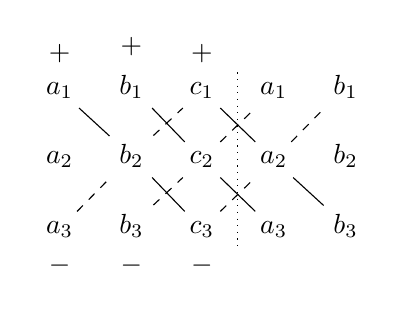
\begin{tikzpicture}
      \matrix [%
        matrix of math nodes,
        column sep=1em,
        row sep=1em
      ] (sarrus) {%
        a_1 & b_1 & c_1 & a_1 & b_1 \\
        a_2 & b_2 & c_2 & a_2 & b_2 \\
        a_3 & b_3 & c_3 & a_3 & b_3 \\
      };

      \path ($(sarrus-1-3.north east)+(0.5em,0)$) edge[dotted] ($(sarrus-3-3.south east)+(0.5em,0)$)
      (sarrus-1-1)                          edge         (sarrus-2-2)
      (sarrus-2-2)                          edge         (sarrus-3-3)
      (sarrus-1-2)                          edge         (sarrus-2-3)
      (sarrus-2-3)                          edge         (sarrus-3-4)
      (sarrus-1-3)                          edge         (sarrus-2-4)
      (sarrus-2-4)                          edge         (sarrus-3-5)
      (sarrus-3-1)                          edge[dashed] (sarrus-2-2)
      (sarrus-2-2)                          edge[dashed] (sarrus-1-3)
      (sarrus-3-2)                          edge[dashed] (sarrus-2-3)
      (sarrus-2-3)                          edge[dashed] (sarrus-1-4)
      (sarrus-3-3)                          edge[dashed] (sarrus-2-4)
      (sarrus-2-4)                          edge[dashed] (sarrus-1-5);

      \foreach \c in {1,2,3} {\node[anchor=south] at (sarrus-1-\c.north) {$+$};};
      \foreach \c in {1,2,3} {\node[anchor=north] at (sarrus-3-\c.south) {$-$};};
    \end{tikzpicture}
  \end{center}

  Note that the Sarrus method is only applicable to 3x3 matrices.

  \subsection{Practice 5}

  Calculate the value of the following determinants.

  \begin{enumerate}
    \item $\vm{
              1 & 5 & 1 \\
              1 & 6 & 3 \\
              9 & 8 & 9
            }$
          \sol{}

          \begin{center}
            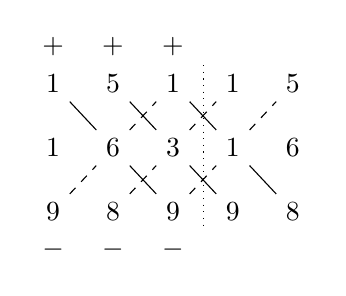
\begin{tikzpicture}
              \matrix [%
                matrix of math nodes,
                column sep=1em,
                row sep=1em
              ] (sarrus) {%
                1 & 5 & 1 & 1 & 5 \\
                1 & 6 & 3 & 1 & 6 \\
                9 & 8 & 9 & 9 & 8 \\
              };

              \path ($(sarrus-1-3.north east)+(0.5em,0)$) edge[dotted] ($(sarrus-3-3.south east)+(0.5em,0)$)
              (sarrus-1-1)                          edge         (sarrus-2-2)
              (sarrus-2-2)                          edge         (sarrus-3-3)
              (sarrus-1-2)                          edge         (sarrus-2-3)
              (sarrus-2-3)                          edge         (sarrus-3-4)
              (sarrus-1-3)                          edge         (sarrus-2-4)
              (sarrus-2-4)                          edge         (sarrus-3-5)
              (sarrus-3-1)                          edge[dashed] (sarrus-2-2)
              (sarrus-2-2)                          edge[dashed] (sarrus-1-3)
              (sarrus-3-2)                          edge[dashed] (sarrus-2-3)
              (sarrus-2-3)                          edge[dashed] (sarrus-1-4)
              (sarrus-3-3)                          edge[dashed] (sarrus-2-4)
              (sarrus-2-4)                          edge[dashed] (sarrus-1-5);

              \foreach \c in {1,2,3} {\node[anchor=south] at (sarrus-1-\c.north) {$+$};};
              \foreach \c in {1,2,3} {\node[anchor=north] at (sarrus-3-\c.south) {$-$};};
            \end{tikzpicture}
          \end{center}
          \begin{flalign*}
            \vm{
            1 & 5                             & 1 \\
            1 & 6                             & 3 \\
            9 & 8                             & 9
            } & = 54 + 135 + 8 - 54 - 24 - 45     \\
              & = 74
          \end{flalign*}
    \item $\vm{
              3 & 1  & -2 \\
              0 & -1 & 1  \\
              4 & 2  & 5
            }$
          \sol{}

          \begin{center}
            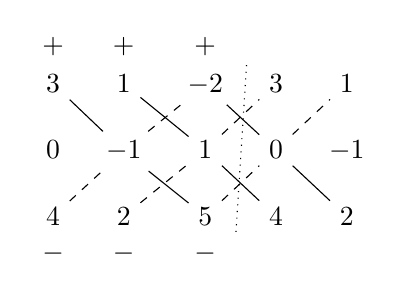
\begin{tikzpicture}
              \matrix [%
                matrix of math nodes,
                column sep=1em,
                row sep=1em
              ] (sarrus) {%
                3 & 1  & -2 & 3 & 1  \\
                0 & -1 & 1  & 0 & -1 \\
                4 & 2  & 5  & 4 & 2  \\
              };

              \path ($(sarrus-1-3.north east)+(0.5em,0)$) edge[dotted] ($(sarrus-3-3.south east)+(0.5em,0)$)
              (sarrus-1-1)                          edge         (sarrus-2-2)
              (sarrus-2-2)                          edge         (sarrus-3-3)
              (sarrus-1-2)                          edge         (sarrus-2-3)
              (sarrus-2-3)                          edge         (sarrus-3-4)
              (sarrus-1-3)                          edge         (sarrus-2-4)
              (sarrus-2-4)                          edge         (sarrus-3-5)
              (sarrus-3-1)                          edge[dashed] (sarrus-2-2)
              (sarrus-2-2)                          edge[dashed] (sarrus-1-3)
              (sarrus-3-2)                          edge[dashed] (sarrus-2-3)
              (sarrus-2-3)                          edge[dashed] (sarrus-1-4)
              (sarrus-3-3)                          edge[dashed] (sarrus-2-4)
              (sarrus-2-4)                          edge[dashed] (sarrus-1-5);

              \foreach \c in {1,2,3} {\node[anchor=south] at (sarrus-1-\c.north) {$+$};};
              \foreach \c in {1,2,3} {\node[anchor=north] at (sarrus-3-\c.south) {$-$};};
            \end{tikzpicture}
          \end{center}
          \begin{flalign*}
            \vm{
            3 & 1                         & -2 \\
            0 & -1                        & 1  \\
            4 & 2                         & 5
            } & = -15 + 4 - 0 - 8 - 6 - 0      \\
              & = -25
          \end{flalign*}
  \end{enumerate}
  \subsection*{Minor and Cofactor}

  The minor of an element in a matrix is the determinant of the matrix obtained
  by deleting the row and column containing the element. Take $\vm{ a_1 & a_2 &
      a_3 \\ b_1 & b_2 & b_3 \\ c_1 & c_2 & c_3 }$ as an example. The minor of $a_1$
  is $\vm{ b_2 & c_2 \\ b_3 & c_3 }$, the minor of $c_2$ is $\vm{ a_1 & b_1 \\
      a_3 & b_3 }$, and so on.

  The cofactor of an element in a matrix is the minor of the element multiplied
  by ${(-1)}^{i+j}$, where $i$ and $j$ are the row and column indices of the
  element. The cofactor of $a_1$ is ${(-1)}^{1+1}\vm{ b_2 & c_2 \\ b_3 & c_3 }$,
  the cofactor of $c_2$ is ${(-1)}^{3+2}\vm{ a_1 & b_1 \\ a_3 & b_3 }$, and so
  on.

  Let $A_1, B_1, C_1$ are the cofactors of $a_1, b_1, c_1$ respectively. Then

  \begin{flalign*}
    A_1 & = (-1)^{1+1}\vm{ b_2 & c_2 \\ b_3 & c_3 } = \vm{ b_2 & c_2 \\ b_3 & c_3 }  \\
    B_1 & = (-1)^{1+2}\vm{ a_2 & c_2 \\ a_3 & c_3 } = -\vm{ a_2 & c_2 \\ a_3 & c_3 } \\
    C_1 & = (-1)^{1+3}\vm{ a_2 & b_2 \\ a_3 & b_3 } = \vm{ a_2 & b_2 \\ a_3 & b_3 }
  \end{flalign*}

  Thus,
  \[|A| =  a_1A_1 + a_2B_1 + a_3C_1\]

  That is, the value of the determinant is the elements of the first row
  multiplied by the cofactors of the elements of the first row.

  The sign of the cofactor is determined by the sum of the row and column indices
  of the element. If the sum is even, the cofactor is positive; if the sum is
  odd, the cofactor is negative.\newline\newline \noindent Generally, a 3x3
  determinant has the following theorem:

  \begin{theorem}
    The determinant of a 3x3 matrix is the sum of the elements of any row or
    column multiplied by the cofactors of the elements of that row or column.
  \end{theorem}

  That is, we can use the cofactor expansion to calculate the determinant of a
  3x3 matrix.

  \begin{flalign*}
    \vm{A} & = a_1A_1 + b_1B_1 + c_1C_1 \\
           & = a_2B_2 + b_2B_2 + c_2C_2 \\
           & = a_3C_3 + b_3C_3 + c_3C_3 \\
           & = a_1A_1 + a_2A_2 + a_3A_3 \\
           & = b_1B_1 + b_2B_2 + b_3B_3 \\
           & = c_1C_1 + c_2C_2 + c_3C_3
  \end{flalign*}

  The determinant of any order matrix can also be calculated by the cofactor
  expansion.

  \begin{theorem}
    The product of the elements of any row or column and the cofactor of corresponding elements of another row or column of a determinant is 0.
  \end{theorem}
  For example, the product of the elements of the second row and the corresponding element of the cofactor of first row of the determinant is 0. That is,
  \begin{flalign*}
     & a_2B_1 + b_2B_1 + c_2C_1                                                      \\
     & = a_2\vm{ b_2                                                           & c_2 \\ b_3 & c_3 } - b_2\vm{ a_2 & c_2 \\ a_3 & c_3 } + c_2\vm{ a_2 & b_2 \\ a_3 & b_3 } \\
     & = a_2b_2c_3 + a_2b_3c_2 - a_2b_2c_3 + a_3b_2c_2 + a_2b_3c_2 - a_3b_2c_2       \\
     & = 0
  \end{flalign*}

  \subsection{Practice 6}
  Find the value of the following 3x3 determinants.

  \begin{enumerate}
    \item $\vm{ 4 & -2 & 1 \\ 1 & -3 & 0 \\ 2 & 7 & -1 }$
          \sol{}
          \begin{flalign*}
             & \vm{ 4                          & -2 & 1 \\ 1 & -3 & 0 \\ 2 & 7 & -1 }                                                                            \\
             & = 4\vm{ - 3                     & 0      \\ 7 & -1 } - \vm{ -2 & 1 \\ 7 & -1 } + 2 \vm{ -2 & 1 \\ -3 & 0 } \\
             & = 4(3 - 0) - (2 - 7) + 2(0 + 3)          \\
             & = 12 + 5 + 6                             \\
             & = 23
          \end{flalign*}

    \item $\vm{ 5 & -4 & 2 \\ 1 & 0 & -3 \\ 1 & -1 & 2 }$
          \sol{}
          \begin{flalign*}
             & \vm{ 5                           & -4 & 2 \\ 1 & 0 & -3 \\ 1 & -1 & 2 }                                                                         \\
             & = 5\vm{ 0                        & -3     \\ -1 & 2 } - \vm{ -4 & 2 \\ -1 & 2 } + \vm{ -4 & 2 \\ 0 & -3 } \\
             & = 5(0 - 3) - (-8 + 2) + (12 + 0)          \\
             & = -15 + 6 + 12                            \\
             & = 3
          \end{flalign*}

    \item $\vm{ 2 & 0 & 1 \\ 0 & 2 & 0 \\ 2 & 0 & -1 }$
          \sol{}
          \begin{flalign*}
             & \vm{ 2              & 0 & 1 \\ 0 & 2 & 0 \\ 2 & 0 & -1 }                                                                         \\
             & = 2\vm{ 2           & 0     \\ 0 & -1 } - 0\vm{ 0 & 1 \\ 0 & -1 } + 2\vm{ 0 & 1 \\ 2 & 0 } \\
             & = 2(-2 - 0) + 2(-2)         \\
             & = -4 - 4                    \\
             & = -8
          \end{flalign*}
  \end{enumerate}

  \subsection{Exercise 14.5a}

  Find the value of the following determinants.

  \begin{enumerate}
    \item $\vm{ 3 & 2 \\ 1 & -4 }$
          \sol{}
          \begin{flalign*}
             & \vm{ 3         & 2 \\ 1 & -4 } \\
             & = 3(-4) - 2(1)     \\
             & = -12 - 2          \\
             & = -14
          \end{flalign*}

    \item $\vm{ 35 & -2 \\ -11 & 5 }$
          \sol{}
          \begin{flalign*}
             & \vm{ 35             & -2 \\ -11 & 5 } \\
             & = 35(5) - (-2)(-11)      \\
             & = 175 - 22               \\
             & = 153
          \end{flalign*}

    \item $\vm{ 1 & a \\ -a & 1 }$
          \sol{}
          \begin{flalign*}
             & \vm{ 1         & a \\ -a & 1 } \\
             & = 1(1) - a(-a)     \\
             & = 1 + a^2          \\
          \end{flalign*}

    \item $\vm{ \sin{x} & -\cos{x} \\ \cos{x} & \sin{x} }$
          \sol{}
          \begin{flalign*}
             & \vm{ \sin{x}                           & -\cos{x} \\ \cos{x} & \sin{x} } \\
             & = \sin{x}\sin{x} - (-\cos{x})(\cos{x})            \\
             & = \sin^2{x} + \cos^2{x}                           \\
             & = 1
          \end{flalign*}

    \item $\vm{ 1 & -2 & 3 \\ 2 & 3 & -4 \\ 3 & -2 & 5 }$
          \sol{}
          \begin{flalign*}
             & \vm{ 1                              & -2 & 3 \\ 2 & 3 & -4 \\ 3 & -2 & 5 }                                                                           \\
             & = 1\vm{ 3                           & -4     \\ -2 & 5 } - 2\vm{ -2 & 3 \\ -2 & 5 } + 3\vm{ -2 & 3 \\ 3 & -4 } \\
             & = 1(15 - 8) - 2(-10 + 6) + 3(8 - 9)          \\
             & = 7 + 8 - 3                                  \\
             & = 12                                         \\
          \end{flalign*}

    \item $\vm{ 1 & -3 & 4 \\ 2 & 0 & -5 \\ 3 & -1 & 7 }$
          \sol{}
          \begin{flalign*}
             & \vm{ 1                             & -3 & 4 \\ 2 & 0 & -5 \\ 3 & -1 & 7 }                                                                          \\
             & = \vm{ 0                           & -5     \\ -1 & 7 } - 2\vm{ -3 & 4 \\ -1 & 7 } + 3\vm{ -3 & 4 \\ 0 & -5 } \\
             & = (0 - 5) - 2(-21 + 4) + 3(15 - 0)          \\
             & = -5 + 34 + 45                              \\
             & = 74
          \end{flalign*}

    \item $\vm{ -1 & 3 & -2 \\ -3 & 2 & 0 \\ 4 & 0 & 5 }$
          \sol{}
          \begin{flalign*}
             & \vm{ -1                          & 3 & -2 \\ -3 & 2 & 0 \\ 4 & 0 & 5 }                                                                       \\
             & = -1\vm{ 2                       & 0      \\ 0 & 5 } + 3\vm{ 3 & -2 \\ 0 & 5 } + 4\vm{ 3 & -2 \\ 2 & 0 } \\
             & = -1(10) + 3(-15 + 0) + 4(0 + 4)          \\
             & = -10 + 45 + 16                           \\
             & = 51
          \end{flalign*}

    \item $\vm{ 0 & -q & -r \\ q & 0 & -s \\ r & s & 0 }$
          \sol{}
          \begin{flalign*}
             & \vm{ 0                      & -q & -r \\ q & 0 & -s \\ r & s & 0 }                                                                          \\
             & = 0\vm{ 0                   & -s      \\ s & 0 } - q\vm{ -q & -r \\ s & 0 } + r\vm{ -q & -r \\ 0 & -s } \\
             & = 0 - q(0 + sr) + r(0 + qs)           \\
             & = 0
          \end{flalign*}

    \item $\vm{ p & -q & r \\ q & r & -s \\ -r & s & p }$
          \sol{}
          \begin{flalign*}
             & \vm{ p                                    & -q & r \\ q & r & -s \\ -r & s & p }                                                                         \\
             & = p\vm{ r                                 & -s     \\ s & p } - q\vm{ -q & r \\ s & p } + r\vm{ -q & r \\ r & -s } \\
             & = p(rp + s^2) -q(-qp - sr) - r(qs - r^2)           \\
             & = rp^2 + p{s}^2 + q^2 p + qsr - qsr + r^3          \\
             & = rp^2 + s^2p + q^2 p - r^3
          \end{flalign*}

    \item $\vm{ 1 & x & a \\ 1 & y & b \\ 1 & z & c }$
          \sol{}
          \begin{flalign*}
             & \vm{ 1                              & x & a \\ 1 & y & b \\ 1 & z & c }                                                                    \\
             & = \vm{ y                            & b     \\ z & c } - \vm{ x & a \\ z & c } + \vm{ x & a \\ y & b } \\
             & = (yc - bz) - (xc - az) + (xb - ay)         \\
             & = bx + cy + az - cx - ay - bz               \\
          \end{flalign*}
  \end{enumerate}

  \subsection*{Identities of Determinants}

  \setcounter{theorem}{0}

  \begin{theorem}
    The value of a determinant is the same as the value of its transpose, aka $|A| = |A'|$.
    \begin{flalign*}
       & \vm{ a & b \\ c & d } = \vm{ a & c \\ b & d }
    \end{flalign*}
  \end{theorem}
  \begin{theorem}
    Switching any two rows or columns of a determinants results in the opposite value.
    \begin{flalign*}
       & \vm{ a_1 & b_1 & c_1 \\ a_2 & b_2 & c_2 \\ a_3 & b_3 & c_3 } = -\vm{ a_1 & b_1 & c_1 \\ a_3 & b_3 & c_3 \\ a_2 & b_2 & c_2 }
    \end{flalign*}
  \end{theorem}

  \subsection{Practice 7}

  Given $\vm{ a & b & c \\ d & e & f \\ g & h & i } = 10$, find $\vm{ b & c & a
      \\ e & f & d \\ h & i & g }$. \sol{}
  \begin{flalign*}
    \vm{
    b & c       & a \\
    e & f       & d \\
    h & i       & g
    }
      & = -\vm{
    a & c       & b \\
    d & f       & e \\
    g & i       & h
    }               \\
      & = \vm{
    a & b       & c \\
    d & e       & f \\
    g & h       & i
    }               \\
      & = 10
  \end{flalign*}
  \begin{theorem}
    If two rows or cols of a determinant are identical, the value of the determinant is zero.
    \begin{flalign*}
       & \vm{ a & b & c \\ a & b & c \\ d & e & f } = 0 \\
    \end{flalign*}
  \end{theorem}
  \begin{theorem}
    If all elements of a row (or column) of a determinant are multiplied by some scalar number k, the value of the new determinant is k times of the given determinant.
    \begin{flalign*}
       & \vm{ a_1 & b_1 & c_1 \\ ka_2 & kb_2 & kc_2 \\ a_3 & b_3 & c_3 } = k\vm{ a_1 & b_1 & c_1 \\ a_2 & b_2 & c_2 \\ a_3 & b_3 & c_3 }
    \end{flalign*}
  \end{theorem}

  \subsection{Practice 8}

  Using the identities of determinants, prove that $\vm{ 10 & -12 & 2 \\ -15 & 18
      & 3 \\ 5 & 6 & -1 } = 180\vm{ 1 & -1 & 1 \\ -1 & 1 & 1 \\ 1 & 1 & -1 }$. \sol{}
  \begin{flalign*}
       & \vm{ 10                        & -12 & 2 \\ -15 & 18 & 3 \\ 5 & 6 & -1 } \\
       & = 5\cdot6\vm{
    2  & -2                             & 2       \\
    -3 & 3                              & 3       \\
    1  & 1                              & -1
    }                                             \\
       & = 5\cdot6\cdot2\cdot3\cdot\vm{
    1  & -1                             & 1       \\
    -1 & 1                              & 1       \\
    1  & 1                              & -1
    }                                             \\
       & = 180\vm{
    1  & -1                             & 1       \\
    -1 & 1                              & 1       \\
    1  & 1                              & -1
    }
  \end{flalign*}

  \begin{theorem}
    In a determinant each element in any row (or column) consists of the sum of two terms, then the determinant can be expressed as sum of two determinants of same order.
    \begin{flalign*}
       & \vm{ a_1+d_1 & b_1 & c_1 \\ a_2+d_2 & b_2 & c_2 \\ a_3+d_3 & b_3 & c_3 } = \vm{ a_1 & b_1 & c_1 \\ a_2 & b_2 & c_2 \\ a_3 & b_3 & c_3 } + \vm{ d_1 & b_1 & c_1 \\ d_2 & b_2 & c_2 \\ d_3 & b_3 & c_3 }
    \end{flalign*}
  \end{theorem}
  \begin{theorem}
    If a determinant is obtained by adding a row or column multiplied by a some scalar number k to a different row or column, then the value of the new determinant is the same as the original determinant.
    \begin{flalign*}
       & \vm{ a_1 & b_1 & c_1 \\ a_2 & b_2 & c_2 \\ a_3 & b_3 & c_3 } = \vm{ a_1+ka_2 & b_1+kb_2 & c_1+kc_2 \\ a_2 & b_2 & c_2 \\ a_3 & b_3 & c_3 }
    \end{flalign*}
  \end{theorem}

  \subsection{Practice 9}

  Prove that $\vm{ 1 & 2 & 3 \\ 4 & 5 & 6 \\ 7 & 8 & 9 } = 0$. \sol{}
  \begin{flalign*}
     & \vm{ 1    & 2                  & 3 \\ 4 & 5 & 6 \\ 7 & 8 & 9 }                                                            \\
     & = \vm{ 1  & 2                  & 3 \\ 3 & 3 & 3 \\ 6 & 6 & 6 }  & (\text{Adding row 1 multiplied by -1 to row 2 and 3}) \\
     & = 2\vm{ 1 & 2                  & 3 \\ 3 & 3 & 3 \\ 3 & 3 & 3 } & (\text{Theorem 4})                                    \\
     & = 0       & (\text{Theorem 3})
  \end{flalign*}

  \begin{theorem}
    The determinant of product of two matrices of equal size is equal to the product of determinants of each matrix, aka $|AB| = |A||B|$.
  \end{theorem}

  \subsection{Practice 10}

  Let $A = \vm{ -2 & 1 \\ 4 & 3 }$ and $B = \vm{ 1 & x \\ 2 & 3 }$. Given that
  $|AB| = -18$, find $x$. \sol{}
  \begin{flalign*}
    \because\ |AB| = |A||B| & = -18 \\
    \therefore\ \vm{
    -2                      & 1     \\
    4                       & 3
    }\vm{
    1                       & x     \\
    2                       & 3
    }                       & = -18 \\
    -2(3-2x)                & = -18 \\
    3-2x                    & = 9   \\
    -2x                     & = 6   \\
    x                       & = -3
  \end{flalign*}

  \subsection{Exercise 14.5b}

  \begin{enumerate}

    \item Given $\vm{ 2 & -2 & 3 \\ 0 & -1 & -2 \\ -1 & 2 & 1 } = -1$, Find the value of
          the following determinants.

          \begin{enumerate}
            \item $\vm{
                      2  & 0  & -1 \\
                      -2 & -1 & 2  \\
                      3  & -2 & 1
                    }$
                  \sol{}
                  \begin{flalign*}
                       & \vm{
                    2  & 0          & -1                 \\
                    -2 & -1         & 2                  \\
                    3  & -2         & 1
                    }                                    \\
                       & =\left|\m{
                    2  & -2         & 3                  \\
                    0  & -1         & -2                 \\
                    -1 & 2          & 1
                    }' \right|                           \\
                       & =-1        & (\text{Theorem 1}) \\
                  \end{flalign*}
            \item $\vm{
                      2  & 0  & -1 \\
                      3  & -2 & 1  \\
                      -2 & -1 & 2
                    }$
                  \sol{}
                  \begin{flalign*}
                       & \vm{
                    2  & 0    & -1 \\
                    3  & -2   & 1  \\
                    -2 & -1   & 2
                    }              \\
                  \end{flalign*}
                  \sol{}
                  \begin{flalign*}
                       & \vm{
                    2  & 0           & -1                 \\
                    3  & -2          & 1                  \\
                    -2 & -1          & 2
                    }                                     \\
                       & = -\vm{
                    2  & 0           & -1                 \\
                    -2 & -1          & 2                  \\
                    3  & -2          & 1
                    }                                     \\
                       & =-\left|\m{
                    2  & -2          & 3                  \\
                    0  & -1          & -2                 \\
                    -1 & 2           & 1
                    }' \right|                            \\
                       & =1          & (\text{Theorem 1}) \\
                  \end{flalign*}
            \item $\vm{
                      4  & -2 & 3  \\
                      0  & -2 & -4 \\
                      -2 & 2  & 1
                    }$
                  \sol{}
                  \begin{flalign*}
                       & \vm{
                    4  & -2            & 3  \\
                    0  & -2            & -4 \\
                    -2 & 2             & 1
                    }  &                    \\
                       & = 2\cdot2\vm{
                    2  & -2            & 3  \\
                    0  & -1            & -2 \\
                    -1 & 2             & 1
                    }  &                    \\
                       & = -4
                  \end{flalign*}
            \item $\vm{
                      -3 & -2 & -2 \\
                      2  & -1 & 0  \\
                      -1 & 2  & 1
                    }$
                  \sol{}
                  \begin{flalign*}
                       & \vm{
                    -3 & -2     & -2 \\
                    2  & -1     & 0  \\
                    -1 & 2      & 1
                    }  &             \\
                       & = \vm{
                    3  & -2     & 2  \\
                    -2 & -1     & 0  \\
                    1  & 2      & -1
                    }  &             \\
                       & = \vm{
                    2  & -2     & 3  \\
                    0  & -1     & -2 \\
                    -1 & 2      & 1
                    }  &             \\
                       & = 1
                  \end{flalign*}
            \item $\vm{
                      0  & 2  & 5  \\
                      0  & -1 & -2 \\
                      -1 & 2  & 1
                    }$
                  \sol{}
                  \begin{flalign*}
                                   & \vm{
                    0              & 2             & 5             \\
                    0              & -1            & -2            \\
                    - 1            & 2             & 1
                    }                                              \\
                                   & = \vm{
                    2+(2\cdot(-1)) & -2+(-2\cdot2) & 3+(2\cdot1) & \\
                    0              & -1            & -2          & \\
                    -1             & 2             & 1
                    }              &                               \\
                                   & = -1
                  \end{flalign*}
            \item $\vm{
                      2  & 4  & 3  \\
                      0  & -5 & -2 \\
                      -1 & 4  & 1
                    }$
                  \sol{}
                  \begin{flalign*}
                       & \vm{
                    2  & 4               & 3    \\
                    0  & -5              & -2   \\
                    -1 & 4               & 1
                    }                           \\
                       & = \vm{
                    2  & -2+(2\cdot3)    & 3  & \\
                    0  & -1+(2\cdot(-2)) & -2 & \\
                    -1 & 2+(2\cdot1)     & 1
                    }  &                        \\
                       & = -1
                  \end{flalign*}
          \end{enumerate}

    \item Prove the following equations using identities of determinants without
          expanding them.

          \begin{enumerate}
            \item $\vm{
                      1 & 0 & 3  \\
                      4 & 6 & 12 \\
                      3 & 3 & 9  \\
                    } = 0$
                  \prooff{}
                  \begin{flalign*}
                    L.H.S. = & \vm{
                    1        & 0                   & 3                  \\
                    4        & 6                   & 12                 \\
                    3        & 3                   & 9                  \\
                    }                                                   \\
                             & = 2\cdot3\vm{
                    1        & 0                   & 3                  \\
                    2        & 3                   & 6                  \\
                    1        & 1                   & 3                  \\
                    }                                                   \\
                             & = 2\cdot3\cdot3\vm{
                    1        & 0                   & 1                  \\
                    2        & 3                   & 2                  \\
                    1        & 1                   & 1                  \\
                    }                                                   \\
                             & = 0 = R.H.S.        & (\text{Theorem 3})
                  \end{flalign*}

            \item $\vm{
                      2  & -1 & 3 \\
                      -1 & 1  & 2 \\
                      4  & -2 & 6
                    } = 0$
                  \prooff{}
                  \begin{flalign*}
                    L.H.S. & = \vm{
                    2      & -1            & 3                  \\
                    -1     & 1             & 2                  \\
                    4      & -2            & 6
                    }                                           \\
                           & = 2\vm{
                    2      & -1            & 3                  \\
                    -1     & 1             & 2                  \\
                    2      & -1            & 3
                    }                                           \\
                           & = 0  = R.H.S. & (\text{Theorem 3})
                  \end{flalign*}

            \item $\vm{
                      3  & 2 & 2 \\
                      9  & 6 & 5 \\
                      12 & 8 & 8
                    } = 0$
                  \prooff{}
                  \begin{flalign*}
                    L.H.S. & = \vm{
                    3      & 2            & 2                  \\
                    9      & 6            & 5                  \\
                    12     & 8            & 8
                    }      &                                   \\
                           & = 4\vm{
                    3      & 2            & 2                  \\
                    9      & 6            & 5                  \\
                    3      & 2            & 2
                    }      &                                   \\
                           & = 0 = R.H.S. & (\text{Theorem 3})
                  \end{flalign*}
            \item $\vm{
                      10 & 8  & 2  \\
                      15 & 12 & 3  \\
                      20 & 32 & 12
                    } = 0$
                  \prooff{}
                  \begin{flalign*}
                    L.H.S. & = \vm{
                    10     & 8                               & 2                  \\
                    15     & 12                              & 3                  \\
                    20     & 32                              & 12
                    }      &                                                      \\
                           & = 2\cdot3\cdot4\vm{
                    5      & 4                               & 1                  \\
                    5      & 4                               & 1                  \\
                    5      & 8                               & 3
                    }      &                                                      \\
                           & = 2\cdot3\cdot4\cdot5\cdot4\vm{
                    1      & 1                               & 1                  \\
                    1      & 1                               & 1                  \\
                    1      & 2                               & 3
                    }      &                                                      \\
                           & = 0 = R.H.S.                    & (\text{Theorem 3})
                  \end{flalign*}
            \item $\vm{
                      1 & -4 & 5  \\
                      2 & 3  & -2 \\
                      7 & 3  & 0
                    } = \vm{
                      -4 & 3  & 3 \\
                      5  & -2 & 0 \\
                      1  & 2  & 7
                    }$
                  \prooff{}
                  \begin{flalign*}
                    L.H.S     & = \vm{
                    1         & -4                 & 5  \\
                    2         & 3                  & -2 \\
                    7         & 3                  & 0
                    }         &                         \\
                              & = -\vm{
                    5         & -4                 & 1  \\
                    -2        & 3                  & 2  \\
                    0         & 3                  & 7
                    }         &                         \\
                              & = \vm{
                    -4        & 5                  & 1  \\
                    3         & -2                 & 2  \\
                    3         & 0                  & 7
                    }         & (\text{Theorem 2})      \\
                              & = \left|\m{
                    -4        & 5                  & 1  \\
                    3         & -2                 & 2  \\
                    3         & 0                  & 7
                    }'\right| & (\text{Theorem 1})      \\
                              & = \vm{
                    -4        & 3                  & 3  \\
                    5         & -2                 & 0  \\
                    1         & 2                  & 7
                    } = R.H.S.
                  \end{flalign*}
            \item $\vm{
                      -6 & 6  & 3  \\
                      0  & -9 & -3 \\
                      3  & -3 & -6
                    } = -27\vm{
                      1  & -1 & 2  \\
                      3  & 0  & 1  \\
                      -2 & 2  & -1 \\
                    }$
                  \prooff{}
                  \begin{flalign*}
                               & L.H.S.              &    \\
                               & = \vm{
                    -6         & 6                   & 3  \\
                    0          & -9                  & -3 \\
                    3          & -3                  & -6
                    }          &                          \\
                               & = 3\cdot3\cdot3\vm{
                    -2         & 2                   & 1  \\
                    0          & -3                  & -1 \\
                    1          & -1                  & -2 \\
                    }          &                          \\
                               & = -27\vm{
                    1          & -1                  & -2 \\
                    0          & -3                  & -1 \\
                    -2         & 2                   & 1
                    }          & (\text{Theorem 2})       \\
                               & = 27\vm{
                    -1         & 1                   & -2 \\
                    -3         & 0                   & -1 \\
                    2          & -2                  & 1
                    }          & (\text{Theorem 2})       \\
                               & = -27\vm{
                    1          & -1                  & 2  \\
                    3          & 0                   & 1  \\
                    -2         & 2                   & -1 \\
                    } = R.H.S. & (\text{Theorem 4})
                  \end{flalign*}
            \item $\vm{
                      1 & 0  & -3 \\
                      3 & -2 & 4  \\
                      1 & 3  & -2
                    } = \vm{
                      1  & 0 & -3 \\
                      -1 & 2 & 4  \\
                      7  & 3 & -2
                    }$
                  \prooff{}
                  \begin{flalign*}
                                     & L.H.S.             &    \\
                                     & = \vm{
                    1                & 0                  & -3 \\
                    3                & -2                 & 4  \\
                    1                & 3                  & -2
                    }                &                         \\
                                     & = \vm{
                    1 + (2\cdot 0)   & 0                  & -3 \\
                    3 + (2\cdot(-2)) & -2                 & 4  \\
                    1 + (2\cdot 3)   & 3                  & -2
                    }                & (\text{Theorem 6})      \\
                                     & = \vm{
                    1                & 0                  & -3 \\
                    -1               & 2                  & 4  \\
                    7                & 3                  & -2
                    }  = R.H.S.
                  \end{flalign*}
            \item $\vm{
                      5 & 1  & -1 \\
                      2 & -1 & -1 \\
                      1 & -2 & 4
                    } = \vm{
                      3 & 1  & 0  \\
                      4 & -1 & -2 \\
                      5 & -2 & 2
                    }$
                  \prooff{}
                  \begin{flalign*}
                                      & L.H.S.             &      \\
                                      & = \vm{
                    5                 & 1                  & -1   \\
                    2                 & -1                 & -1   \\
                    1                 & -2                 & 4
                    }                 &                           \\
                                      & = \vm{
                    5 + (-2\cdot 1)   & 1                  & -1+1 \\
                    2 + (-2\cdot(-1)) & -1                 & -2-1 \\
                    1 + (-2\cdot(-2)) & -2                 & 4-2
                    }
                                      & (\text{Theorem 6})        \\
                                      & = \vm{
                    3                 & 1                  & 0    \\
                    4                 & -1                 & -2   \\
                    5                 & -2                 & 2
                    } = R.H.S.
                  \end{flalign*}
          \end{enumerate}
    \item Let $A = \m{ 7 & -4 \\ -3 & 2 }$ and $B = \m{ 2x+1 & -2 \\ x & 1 }$. Given that
          $|AB| = -22$, find the value of x. \sol{}
          \begin{flalign*}
            \because\ |AB|                = |A||B| & = -22 & \\
            \therefore\ \vm{
            7                                      & -4      \\
            -3                                     & 2
            }\vm{
            2x+1                                   & -2      \\
            x                                      & 1
            }                                      & = -22 & \\
            2(2x+1 + 2x)                           & = -22 & \\
            4x + 1                                 & = -11 & \\
            4x                                     & = -12 & \\
            x                                      & = -3  & \\
          \end{flalign*}
    \item Let $P = \m{ 3a & 3b & 3c \\ d & e & f \\ g & h & i }$ and $Q = \m{ a & d & g
              \\ b & e & h \\ c & f & i }$. Given that $PQ = \m{ 30 & -18 & -33 \\ -6 & 4 & 6
              \\ -11 & 6 & 14 }$, find the value of $|Q|$. \sol{}
          \begin{flalign*}
            \because\ |P||Q| & = |PQ|      &     \\
            \therefore\ \vm{
            3a               & 3b          & 3c  \\
            d                & e           & f   \\
            g                & h           & i
            }\vm{
            a                & d           & g   \\
            b                & e           & h   \\
            c                & f           & i
            }                & = \vm{
            30               & -18         & -33 \\
            -6               & 4           & 6   \\
            -11              & 6           & 14
            }                &                   \\
            3\vm{
            a                & b           & c   \\
            d                & e           & f   \\
            g                & h           & i
            }\vm{
            a                & b           & c   \\
            d                & e           & f   \\
            g                & h           & i
            }                & = \vm{
            30               & -18         & -33 \\
            -6               & 4           & 6   \\
            -11              & 6           & 14
            }                &                   \\
            3{\left(\vm{
            a                & b           & c   \\
            d                & e           & f   \\
            g                & h           & i
            }\right)}^2      & = 3\vm{
            10               & -6          & -11 \\
            -6               & 4           & 6   \\
            -11              & 6           & 14
            }                &                   \\
            {\left(\vm{
            a                & b           & c   \\
            d                & e           & f   \\
            g                & h           & i
            }\right)}^2      & = \vm{
            10               & -6          & -11 \\
            -6               & 4           & 6   \\
            -11              & 6           & 14
            }                &                   \\
                             & =4          &     \\
            \therefore\ |Q|  & = \vm{
            a                & d           & g   \\
            b                & e           & h   \\
            c                & f           & i
            }                &                   \\
                             & = \left|\m{
            a                & b           & c   \\
            d                & e           & f   \\
            g                & h           & i
            }'\right|        &                   \\
                             & =\vm{
            a                & b           & c   \\
            d                & e           & f   \\
            g                & h           & i
            }                &                   \\
                             & = \pm{2}    &     \\
          \end{flalign*}
          Find the value of x in the following equations.
    \item $\vm{
              x   & x  \\
              -2x & -1
            } = 6$
          \sol{}
          \begin{flalign*}
            \vm{
            x                   & x                \\
            -2x                 & -1
            }                   & = 6            & \\
            x\vm{
            1                   & 1                \\
            -2x                 & -1
            }                   & = 6            & \\
            x(-1+2x)            & = 6            & \\
            -x + 2x^2           & = 6            & \\
            2x^2 - x - 6        & = 0            & \\
            (x-2)(2x+3)         & = 0            & \\
            x = 2 \text{ or } x & = -\frac{3}{2} & \\
          \end{flalign*}
    \item $\vm{
              2 & 4 & 0 \\
              2 & 5 & 6 \\
              3 & x & 9
            } = 0$
          \sol{}
          \begin{flalign*}
            \vm{
            2                 & 4              & 0 \\
            2                 & 5              & 6 \\
            3                 & x              & 9
            }                 & = 0            &   \\
            2\cdot3\vm{
            1                 & 2              & 0 \\
            2                 & 5              & 2 \\
            3                 & x              & 3
            }                 & =0             &   \\
            \vm{
            1                 & 2              & 0 \\
            2                 & 5              & 2 \\
            3                 & x              & 3
            }                 & =0             &   \\
            \vm{
            5                 & 2                  \\
            x                 & 3
            } - 2\vm{
            2                 & 0                  \\
            x                 & 3
            }
            + 3\vm{
            2                 & 0                  \\
            5                 & 2
            }                 & =0             &   \\
            15 - 2x - 12 + 12 & =0             &   \\
            -2x               & = -15          &   \\
            x                 & = \frac{15}{2} &   \\
          \end{flalign*}
    \item $\vm{
              1 & 1 & x \\
              1 & x & 1 \\
              x & 1 & 1
            } = 0$
          \sol{}
          \begin{flalign*}
            \vm{
            1                       & 1   & x \\
            1                       & x   & 1 \\
            x                       & 1   & 1
            }                       & = 0 &   \\
            \vm{
            x                       & 1       \\
            1                       & 1
            } - \vm{
            1                       & x       \\
            1                       & 1
            }
            + x\vm{
            1                       & x       \\
            x                       & 1
            }                       & = 0 &   \\
            x - 1 - 1 + x + x - x^3 & = 0 &   \\
            -x^3 + 3x - 2           & = 0 &   \\
            x^3 - 3x + 2            & = 0 &   \\
            (x+2)(x^2-2x+1)         & = 0 &   \\
            x = -2 \text{ or } x    & = 1 &   \\
          \end{flalign*}
    \item $\vm{
              2x-7 & 6 & 9 \\
              3x-5 & 5 & 4 \\
              x-3  & 0 & 1
            } = 0$
          \sol{}
          \begin{flalign*}
            \vm{
            2x-7             & 6     & 9 \\
            3x-5             & 5     & 4 \\
            x-3              & 0     & 1
            }                & = 0   &   \\
            \vm{
            2x               & 6     & 9 \\
            3x               & 5     & 4 \\
            x                & 0     & 1
            } + \vm{
            -7               & 6     & 9 \\
            -5               & 5     & 4 \\
            -3               & 0     & 1
            }                & = 0   &   \\
            \vm{
            2x               & 6     & 9 \\
            3x               & 5     & 4 \\
            x                & 0     & 1
            }                & = -58 &   \\
            x\vm{
            6                & 9         \\
            5                & 4
            } + \vm{
            2x               & 6         \\
            3x               & 5
            }                & = -58 &   \\
            -21x + 10x - 18x & = -58 &   \\
            -29x             & = -58 &   \\
            x                & = 2   &   \\
          \end{flalign*}
    \item $\vm{
              15-2x & 11 & 10 \\
              11-3x & 17 & 16 \\
              7-x   & 14 & 13
            } = 0$
          \sol{}
          \begin{flalign*}
            \vm{
            15-2x         & 11    & 10 \\
            11-3x         & 17    & 16 \\
            7-x           & 14    & 13
            }             & = 0   &    \\
            \vm{
            15            & 11    & 10 \\
            11            & 17    & 16 \\
            7             & 14    & 13
            } + \vm{
            -2x           & 11    & 10 \\
            -3x           & 17    & 16 \\
            -x            & 14    & 13
            }             & = 0   &    \\
            \vm{
            -2x           & 11    & 10 \\
            -3x           & 17    & 16 \\
            -x            & 14    & 13
            } = 36        &            \\
            -2x \vm{
            17            & 16         \\
            14            & 13
            } + 3x\vm{
            11            & 10         \\
            14            & 13
            } - x\vm{
            11            & 10         \\
            17            & 16
            }             & = 36  &    \\
            x\left(2 \vm{
            17            & 16         \\
            14            & 13
            } - 3\vm{
            11            & 10         \\
            14            & 13
            } + \vm{
            11            & 10         \\
            17            & 16
            }\right)      & = -36 &    \\
            (-6 - 9 + 6)x & = -36 &    \\
            -9x           & = -36 &    \\
            x             & = 4   &    \\
          \end{flalign*}
    \item $\vm{
              x-1 & 0   & x-3 \\
              1   & x-2 & 1   \\
              2   & x-2 & 2
            } = 0$
          \sol{}
          \begin{flalign*}
            \vm{
            x-1                                        & 0   & x-3 \\
            1                                          & x-2 & 1   \\
            2                                          & x-2 & 2
            }                                          & = 0 &     \\
            (x-2)\vm{
            x-1                                        & 0   & x-3 \\
            1                                          & 1   & 1   \\
            2                                          & 1   & 2
            }                                          & = 0 &     \\
            (x-2)\left(
            -\vm{
            x-1                                        & x-3       \\
            2                                          & 2
            }
            + \vm{
            x-1                                        & x-3       \\
            1                                          & 1
            }
            \right)                                    & = 0 &     \\
            (x-2)\left[-(2x-2-2x+6) + (x-1-x-3)\right] & = 0 &     \\
            (x-2)                                      & = 0 &     \\
            x                                          & = 2 &     \\
          \end{flalign*}
  \end{enumerate}

  \section{Inverse Matrix}

  If two square matrices $A$ and $B$ are of the same order such that $AB=BA=I$,
  while $I$ is an identity matrix that has the same order as $A$ and $B$, then
  $A$ and $B$ are said to be inverse matrices of each other, and can be denoted
  as $B = A^{-1}$ and $A = B^{-1}$.

  Note that only square matrix have inverse matrix. If a matrix has an inverse
  matrix, then it is said to be invertible, and the inverse matrix is unique.

  \subsection*{Inverse Matrix of a 2x2 Matrix}

  Let $A = \m{ a & b \\ c & d }$ be a 2x2 matrix. Then
  \[
    A^{-1} = \frac{1}{ad-bc} \m{ d & -b \\ -c & a }
    \ \ \ \ \ (ad-bc \neq 0)
  \]

  If $|A| = ad - bc = 0$, then $A$ is said to be non-invertible.

  \subsection{Practice 11}

  Determine if the following matrices are invertible. If they are, find their
  inverse matrices.

  \begin{enumerate}
    \item $\m{ 6 & 3 \\ 7 & 5 }$
          \sol{}
          \begin{flalign*}
            |A|           & = 6 \cdot 5 - 3 \cdot 7 = 9 \neq 0                \\
            \therefore\ A & \text{ is invertible.}                            \\
            A^{-1}        & = \frac{1}{9} \m{ 5                & -3           \\ -7 & 6 }                             \\
                          & = \m{ \frac{5}{9}                  & -\frac{1}{1} \\ -\frac{7}{9} & \frac{2}{3} }
          \end{flalign*}
    \item $\m{
              -3 & -2 \\
              6  & 4
            }$
          \sol{}
          \begin{flalign*}
            |A|           & = -3 \cdot 4 - (-2) \cdot 6 = 0 \\
            \therefore\ A & \text{ is non-invertible.}
          \end{flalign*}
    \item $\m{ 2 & -6 \\ 3 & -5 }$
          \sol{}
          \begin{flalign*}
            |A|           & = 2 \cdot -5 - (-6) \cdot 3 = 8 \neq 0               \\
            \therefore\ A & \text{ is invertible.}                               \\
            A^{-1}        & = \frac{1}{8} \m{ -5                   & 6           \\ -3 & 2 }                             \\
                          & = \m{ -\frac{5}{8}                     & \frac{3}{4} \\ -\frac{3}{8} & \frac{1}{4} }
          \end{flalign*}

    \item If $\m{ 2b+1 & 2 \\ -3b-3 & -4 }$ is non-invertible, find the value of $b$.
          \sol{}
          \begin{flalign*}
            \because\ \text{The matrix is no} & \text{n-invertible} \\
            \therefore\ \vm{
            2b+1                              & 2                   \\
            -3b-3                             & -4
            }                                 & = 0                 \\
            -8b -4 + 6b + 6                   & = 0                 \\
            -2b + 2                           & = 0                 \\
            b                                 & = 1
          \end{flalign*}
  \end{enumerate}
  \subsection*{Inverse Matrix of a 3x3 Matrix}

  Let a 3x3 matrix $A$ be of the form $A = \m{ a_1 & b_1 & c_1 \\ a_2 & b_2 & c_2
      \\ a_3 & b_3 & c_3 }$. Arrange all the cofactors of elements in $A$ into a
  matrix:
  \[
    \m{
      A_1 & B_1 & C_1 \\
      A_2 & B_2 & C_2 \\
      A_3 & B_3 & C_3
    }
  \]

  Then the transpose of the matrix is the adjoint matrix of $A$, and can be
  denoted as $\operatorname{adj}A$. That is:
  \[
    \operatorname{adj}A = \m{
      A_1 & A_2 & A_3 \\
      B_1 & B_2 & B_3 \\
      C_1 & C_2 & C_3
    }
  \]
  The inverse matrix of $A$ is:
  \[
    A^{-1} = \frac{1}{|A|} \operatorname{adj}A
    \ \ \ \ \ (|A| \neq 0)
  \]

  \subsection{Practice 12}

  Find the inverse matrix of the following matrices.

  \begin{enumerate}
    \item $\m{
              -1 & 2  & 3  \\
              3  & 0  & 1  \\
              2  & -1 & -2
            }$
          \sol{}
          \begin{flalign*}
                                        & |A| = \vm{
            -1                          & 2                & 3           \\
            3                           & 0                & 1           \\
            2                           & -1               & -2          \\
            } = 6                       &                                \\
                                        & \m{
            \vm{ 0                      & 1                              \\ -1 & -2 }  & -\vm{ 3 & 1 \\ 2 & -2 } & \vm{ 3 & 0 \\ 2 & -1 }   \\
            -\vm{ 2                     & 3                              \\ -1 & -2 } & \vm{ -1 & 3 \\ 2 & -2 } & -\vm{ -1 & 2 \\ 2 & -1 } \\
            \vm{ 2                      & 3                              \\ 0 & 1 }    & -\vm{ -1 & 3 \\ 3 & 1 } & \vm{ -1 & 2 \\ 3 & 0 }
            }                                                            \\
                                        & =\m{
            1                           & 8                & -3          \\
            1                           & -4               & 3           \\
            2                           & 10               & -6
            }                           &                                \\
            \operatorname{adj}A         & = \m{
            1                           & 1                & 2           \\
            8                           & -4               & 10          \\
            -3                          & 3                & -6
            }                           &                                \\
            \therefore\          A^{-1} & = \frac{1}{6}\m{
            1                           & 1                & 2           \\
            8                           & -4               & 10          \\
            -3                          & 3                & -6
            } = \m{
            \frac{1}{6}                 & \frac{1}{6}      & \frac{1}{3} \\
            \frac{4}{3}                 & -\frac{2}{3}     & \frac{5}{3} \\
            -\frac{1}{2}                & \frac{1}{2}      & -1
            }
          \end{flalign*}
    \item $\m{
              1  & -2 & -1 \\
              -1 & 2  & -3 \\
              1  & 0  & 1
            }$
          \sol{}
          \begin{flalign*}
                                        & |A| = \vm{
            1                           & -2               & -1          \\
            -1                          & 2                & -3          \\
            1                           & 0                & 1
            } = 8                       &                                \\
                                        & \m{
            \vm{ 2                      & -3                             \\ 0 & 1 }   & -\vm{ -1 & -3 \\ 1 & 1 }  & \vm{ -1 & 2 \\ 1 & 0 }  \\
            -\vm{ -2                    & -1                             \\ 0 & 1 } & \vm{ 1 & -1 \\ 1 & 1 }    & -\vm{ 1 & -2 \\ 1 & 0 } \\
            \vm{ -2                     & -1                             \\ 2 & -3 } & -\vm{ 1 & -1 \\ -1 & -3 } & \vm{ 1 & -2 \\ -1 & 2 }
            }                           &                                \\
                                        & = \m{
            2                           & -2               & -2          \\
            2                           & 2                & -2          \\
            8                           & 4                & 0
            }                           &                                \\
            \operatorname{adj}A         & = \m{
            2                           & 2                & 8           \\
            -2                          & 2                & 4           \\
            -2                          & -2               & 0
            }                           &                                \\
            \therefore\          A^{-1} & = \frac{1}{8}\m{
            2                           & 2                & 8           \\
            -2                          & 2                & 4           \\
            -2                          & -2               & 0
            } = \m{
            \frac{1}{4}                 & \frac{1}{4}      & 1           \\
            -\frac{1}{4}                & \frac{1}{4}      & \frac{1}{2} \\
            -\frac{1}{4}                & -\frac{1}{4}     & 0
            }
          \end{flalign*}
  \end{enumerate}

  \subsection*{Solving Systems of Linear Equations}

  Binary and ternary systems of linear equations can be solved by using the
  inverse matrix of the coefficient matrix. Note that the coefficient matrix must
  be invertible for this method to work.

  \subsection{Practice 13}

  Solve the following systems of linear equations using the inverse matrix
  method.

  \begin{enumerate}
    \item $\begin{cases}
              3x - 2y = 12 \\
              7x + 5y = -1
            \end{cases}$
          \sol{}
          \begin{flalign*}
            \text{Let } A & = \m{
            3             & -2                \\
            7             & 5
            }                                 \\
            A\m{
            x                                 \\
            y
            }             & = \m{
            12                                \\
            -1
            }                                 \\
            A^{-1}A\m{
            x                                 \\
            y
            }             & = A^{-1}\m{
            12                                \\
            -1
            }                                 \\
            \m{
            x                                 \\
            y
            }             & = A^{-1}\m{
            12                                \\
            -1
            }                                 \\
                          & = \frac{1}{29}\m{
            5             & 2                 \\
            -7            & 3
            }\m{
            12                                \\
            -1
            }                                 \\
                          & = \frac{1}{29}\m{
            58                                \\
            -87
            }                                 \\
                          & = \m{
            2                                 \\
            -3
            }                                 \\
            \therefore\ x & = 2,\ y = -3
          \end{flalign*}
    \item $\begin{cases}
              x + y + z = 6  \\
              2x - y + z = 3 \\
              x - y - 2z = -7
            \end{cases}$
          \sol{}
          \begin{flalign*}
            \text{Let } A & = \m{
            1             & 1                   & 1            \\
            2             & -1                  & 1            \\
            1             & -1                  & -2
            }                                                  \\
            A\m{
            x                                                  \\
            y                                                  \\
            z
            }             & = \m{
            6                                                  \\
            3                                                  \\
            -7
            }                                                  \\
            A^{-1}A\m{
            x                                                  \\
            y                                                  \\
            z
            }             & = A^{-1}\m{
            6                                                  \\
            3                                                  \\
            -7
            }                                                  \\
            \m{
            x                                                  \\
            y                                                  \\
            z
            }             & = A^{-1}\m{
            6                                                  \\
            3                                                  \\
            -7
            }                                                  \\
                          & = \m{
            \frac{3}{7}   & \frac{1}{7}         & \frac{2}{7}  \\
            \frac{5}{7}   & -\frac{3}{7}        & \frac{1}{7}  \\
            -\frac{1}{7}  & \frac{2}{7}         & -\frac{3}{7}
            }
            \m{
            6                                                  \\
            3                                                  \\
            -7
            }                                                  \\
                          & = \m{
            1                                                  \\
            2                                                  \\
            3
            }                                                  \\
            \therefore\ x & = 1,\ y = 2,\ z = 3
          \end{flalign*}
  \end{enumerate}

  \subsection{Exercise 14.6}

  Determine if the following second-order matrices are invertible. If they are,
  find their inverse matrix.

  \begin{enumerate}
    \item $\m{
              5 & 2 \\
              7 & 3
            }$
          \sol{}
          \begin{flalign*}
            |A|           & = 5 \cdot 3 - 2 \cdot 7 = 1 \neq 0 & \\
            \therefore\ A & \text{ is invertible}              & \\
            A^{-1}        & = \m{
            3             & -2                                   \\
            -7            & 5
            }
          \end{flalign*}

    \item $\m{
              4  & -8 \\
              -1 & 2
            }$
          \sol{}
          \begin{flalign*}
            |A|           & = 4 \cdot 2 - (-8) \cdot (-1) = 0 & \\
            \therefore\ A & \text{ is not invertible}         & \\
          \end{flalign*}

    \item $\m{
              10 & 5  \\
              -6 & -3
            }$
          \sol{}
          \begin{flalign*}
            |A|           & = 10 \cdot (-3) - 5 \cdot (-6) = 0 & \\
            \therefore\ A & \text{ is not invertible}          & \\
          \end{flalign*}

    \item $\m{
              4  & -5 \\
              -7 & 9
            }$
          \sol{}
          \begin{flalign*}
            |A|           & = 4 \cdot 9 - (-5) \cdot (-7) = 1 \neq 0 & \\
            \therefore\ A & \text{ is invertible}                    & \\
            A^{-1}        & = \m{
            9             & 5                                          \\
            7             & 4
            }
          \end{flalign*}

    \item $\m{
              -2 & -1 \\
              6  & 3
            }$
          \sol{}
          \begin{flalign*}
            |A|           & = (-2) \cdot 3 - (-1) \cdot 6 = 0 & \\
            \therefore\ A & \text{ is not invertible}         & \\
          \end{flalign*}

    \item $\m{
              \sin{\alpha} & -\cos{\alpha} \\
              \cos{\alpha} & \sin{\alpha}
            }$
          \sol{}
          \begin{flalign*}
            |A|           & = \sin{\alpha} \cdot \sin{\alpha} - (-\cos{\alpha}) \cdot \cos{\alpha} = 1 \neq 0 & \\
            \therefore\ A & \text{ is invertible}                                                             & \\
            A^{-1}        & = \m{
            \sin{\alpha}  & \cos{\alpha}                                                                        \\
            -\cos{\alpha} & \sin{\alpha}
            }
          \end{flalign*}

    \item Given that the inverse matrix of matrix $\m{ -2 & 5 \\ 1 & x }$ is $\m{ x & y
              \\ -1 & -2 }$, find the value of $x$ and $y$. \sol{}
          \begin{flalign*}
            \vm{
            -2            & 5                          \\
            1             & x
            }             & = -2x - 5                  \\
            (-2x-5)\m{
            x             & -5                         \\
            -1            & -2
            }             & = \m{
            x             & y                          \\
            -1            & -2
            }                                          \\
            \m{
            -2x^2 - 10x   & 10x + 25                   \\
            2x + 5        & 4x + 10
            }             & = \m{
            x             & y                          \\
            -1            & -2
            }                                          \\
            \text{Comparing coefficients,}             \\
            \begin{cases}
              -2x^2 - 10x = x  & \\
              10x + 25    = y  & \\
              2x + 5      = -1 & \\
              4x + 10     = -2 &
            \end{cases}   \\
            2x            & = -6                       \\
            x             & = -3                       \\
            -30 + 25      & = y                        \\
            y             & = -5                       \\
            \therefore\ x & = -3,\ y              = -5
          \end{flalign*}

    \item If the matrix $\m{ 3 & x \\ -2 & 4 }$ is not invertible, find the value of $x$.
          \sol{}
          \begin{flalign*}
            \vm{
            3       & x                              \\
            -2      & 4
            }       & = 3 \cdot 4 - x \cdot (-2) = 0 \\
            12 + 2x & = 0                            \\
            x       & = -6                           \\
          \end{flalign*}

    \item Given the matrix $\m{ y^2 - 7 & -2 \\ 6 & 2y }$, find the range of $y$ such
          that the matrix is invertible. \sol{}
          \begin{flalign*}
            \vm{
            y^2 - 7           & -2                               \\
            6                 & 2y
            }                 & = (y^2 - 7) \cdot 2y + 12 \neq 0 \\
            y^3 - 7y + 6      & \neq 0                           \\
            (y-1)(y+3)(y-2)   & \neq 0                           \\
            y \in \mathbb{R}, & \ y \neq -3, 1, 2
          \end{flalign*}

    \item Given the matrix $\m{ x & 2 & 1 \\ -1 & x-1 & -2 \\ 1-x & 1 & 1 }$, find the
          range of $x$ such that the matrix is not invertible. \sol{}
          \begin{flalign*}
                & \vm{
            x   & 2                                              & 1  \\
            -1  & x-1                                            & -2 \\
            1-x & 1                                              & 1
            }   &                                                     \\
                & = \vm{
            -1  & x-1                                                 \\
            1-x & 1
            } + 2\vm{
            x   & 2                                                   \\
            1-x & 1
            } + \vm{
            x   & 2                                                   \\
            -1  & x-1
            }   &                                                     \\
                & = 1 + x^2 - 2x + 1 + 2x - 4 + 4x + x^2 - x + 2 &    \\
                & = 2x^2 + 3x - 4 = 0                            &    \\
                & \ \ (x+2)(2x-1)  = 0                           &    \\
                & \ \ x  = -2 \text{ or } x = \frac{1}{2}        &    \\
          \end{flalign*}

    \item Given an identity matrix $I = \m{ 1 & 0 \\ 0 & 1 }$, $J = \m{ 0 & 1 \\ -1 & 0
            }$, and $A = \m{ a & 1 \\ 1 & b }$. If $AJA = J$, and $A + A^{-1} = 3I$, find
          $A$. \sol{}
          \begin{flalign*}
            AJA                          & = J                              & \\
            A^{-1}AJA                    & = A^{-1}J                        & \\
            JA = A^{-1}J                 &                                    \\
            A^{-1}                       & = 3I - A                         & \\
                                         & = \m{
            3 - a                        & -1                                 \\
            -1                           & 3 - b
            }                            &                                    \\
            \m{
            0                            & 1                                  \\
            -1                           & 0
            }\m{
            a                            & 1                                  \\
            1                            & b
            }                            & = \m{
            3 - a                        & -1                                 \\
            -1                           & 3 - b
            }\m{
            0                            & 1                                  \\
            -1                           & 0
            }                            &                                    \\
            \m{
            1                            & b                                  \\
            -a                           & -1
            }                            & = \m{
            1                            & 3-a                                \\
            -3+b                         & -1
            }                            &                                    \\
            b                            & = 3-a                            & \\
            \m{
            a                            & 1                                  \\
            1                            & b
            }                            & + \frac{1}{ab - 1} \m{
            b                            & -1                                 \\
            -1                           & a
            } = 3I                       &                                    \\
            \m{
            a                            & 1                                  \\
            1                            & b
            } + \m{
            \frac{b}{ab-1}               & \frac{-1}{ab-1}                    \\
            \frac{-1}{ab-1}              & \frac{a}{ab-1}
            }                            & = \m{
            3                            & 0                                  \\
            0                            & 3
            }                            &                                    \\
            \m{
            \frac{a^2b - a + b}{ab-1}    & \frac{ab - 2}{ab-1}              & \\
            \frac{ab - 2}{ab-1}          & \frac{ab^2 - b + a}{ab-1}
            }                            & = \m{
            3                            & 0                                  \\
            0                            & 3
            }                            &                                    \\
            \frac{ab - 2}{ab-1}          & = 0                              & \\
            a(3-a) -2                    & = 0                              & \\
            a^2 -3a +2                   & = 0                              & \\
            (a-2)(a-1)                   & = 0                              & \\
            a                            & = 2 \text{ or } a = 1            & \\
            \text{When } a = 2, \ b = 1, & \text{ and when } a = 1, \ b = 2 & \\
            \therefore\ A = \m{
            2                            & 1                                  \\
            1                            & 1
            }                            & \text{ or } A = \m{
            1                            & 1                                  \\
            1                            & 2
            }
          \end{flalign*}

    \item Given that $A = \m{ a & b & c \\ d & e & f \\ g & h & i }$, $B = \m{ 1 & 3 & 2
              \\ 0 & 1 & 0 \\ 1 & 0 & 3 }$, and $C = \m{ 1 & 0 & 3 \\ 1 & -1 & 2 \\ -2 & -1 &
              1 }$, if $AB = C$, find $A$. \sol{}
          \begin{flalign*}
            AB       & = C            \\
            ABB^{-1} & = CB^{-1}      \\
            A        & = CB^{-1}      \\
            A        & = \m{
            1        & 0         & 3  \\
            1        & -1        & 2  \\
            -2       & -1        & 1
            }\m{
            3        & -9        & -2 \\
            0        & 1         & 0  \\
            -1       & 3         & 1
            }                         \\
                     & = \m{
            0        & 0         & 1  \\
            1        & -4        & 0  \\
            -7       & 20        & 5
            }                         \\
          \end{flalign*}

          Find the inverse matrix of the following matrices.

    \item $\m{
              1 & 0 & 2 \\
              4 & 1 & 3 \\
              2 & 1 & 0
            }$
          \sol{}
          \begin{flalign*}
                         & \vm{
            1            & 0                          & 2  \\
            4            & 1                          & 3  \\
            2            & 1                          & 0
            } = 1                                          \\
                         & \m{
            \vm{1        & 3                               \\1&0}  & -\vm{4&3\\2&0} & \vm{4&1\\2&1}  \\
            -\vm{0       & 2                               \\1&0} & \vm{1&2\\2&0}  & -\vm{1&0\\2&1} \\
            \vm{0        & 2                               \\1&3}  & -\vm{1&2\\4&3} & \vm{1&0\\4 & 1}
            }                                              \\
                         & = \m{
            3            & -6                         & 2  \\
            -2           & -4                         & -1 \\
            -2           & 5                          & 1
            }                                              \\
                         & \operatorname{adj} A = \m{
            3            & -2                         & -2 \\
            -6           & -4                         & 5  \\
            2            & -1                         & 1
            }                                              \\
            \therefore\  & A^{-1} = \m{
            3            & -2                         & -2 \\
            -6           & -4                         & 5  \\
            2            & -1                         & 1
            }                                              \\
          \end{flalign*}

    \item $\m{
              1  & 2 & -1 \\
              3  & 1 & 0  \\
              -1 & 0 & -2
            }$
          \sol{}
          \begin{flalign*}
                         & \vm{
            1            & 2                          & -1           \\
            3            & 1                          & 0            \\
            -1           & 0                          & -2
            } = 9                                                    \\
                         & \m{
            \vm{1        & 0                                         \\0&-2}   & -\vm{3&0\\-1&-2} & \vm{3&1\\-1&0}  \\
            -\vm{2       & -1                                        \\0&-2} & \vm{1&-1\\-1&-2} & -\vm{1&2\\-1&0} \\
            \vm{2        & -1                                        \\1&0}   & -\vm{1&-1\\3&0}  & \vm{1&2\\3 & 1}
            }                                                        \\
                         & = \m{
            -2           & 5                          & 1            \\
            4            & -3                         & -2           \\
            1            & -3                         & -5
            }                                                        \\
                         & \operatorname{adj} A = \m{
            -2           & 4                          & 1            \\
            6            & -3                         & -3           \\
            1            & -2                         & -5
            }                                                        \\
            \therefore\  & A^{-1} = \frac{1}{9}\m{
            -2           & 4                          & 1            \\
            6            & -3                         & -3           \\
            1            & -2                         & -5
            }                                                        \\
                         & = \m{
            -\frac{1}{9} & \frac{4}{9}                & \frac{1}{9}  \\
            \frac{2}{5}  & -\frac{1}{3}               & -\frac{1}{3} \\
            \frac{1}{9}  & -\frac{2}{9}               & -\frac{5}{9}
            }
          \end{flalign*}

    \item $\m{
              1 & -1 & 3 \\
              0 & -4 & 3 \\
              2 & 3  & 1
            }$
          \sol{}
          \begin{flalign*}
                          & \vm{
            1             & -1                         & 3            \\
            0             & -4                         & 3            \\
            2             & 3                          & 1
            } = 5                                                     \\
                          & \m{
            \vm{-4        & 3                                         \\3&1}  & -\vm{0&3\\2&1} & \vm{0&-4\\2&3}  \\
            -\vm{-1       & 3                                         \\3&1} & \vm{1&3\\2&1}  & -\vm{1&-1\\2&3} \\
            \vm{-1        & 3                                         \\-4&3} & -\vm{1&3\\0&3} & \vm{1&-1\\0 & -4}
            }                                                         \\
                          & = \m{
            -13           & 6                          & 8            \\
            10            & -5                         & -5           \\
            9             & -3                         & -4
            }                                                         \\
                          & \operatorname{adj} A = \m{
            -13           & 10                         & 9            \\
            6             & -5                         & -3           \\
            8             & -5                         & -4
            }                                                         \\
            \therefore\   & A^{-1} = \frac{1}{5}\m{
            -13           & 10                         & 9            \\
            6             & -5                         & -3           \\
            8             & -5                         & -4
            }                                                         \\
                          & = \m{
            -\frac{13}{5} & \frac{10}{5}               & \frac{9}{5}  \\
            \frac{6}{5}   & -\frac{1}{5}               & -\frac{3}{5} \\
            \frac{8}{5}   & -\frac{1}{5}               & -\frac{4}{5}
            }
          \end{flalign*}

          Solve the following systems of linear equations using the inverse matrix
          method.

    \item $\begin{cases}
              3x + 2y = 1 \\
              4x -y = 5
            \end{cases}$
          \sol{}
          \begin{flalign*}
            \text{Let } A & = \m{
            3             & 2                  \\
            4             & -1
            }                                  \\
            A\m{x                              \\y}       & = \m{1\\5}                           \\
            A^{-1}A\m{x                        \\y} & = A^{-1}\m{1\\5}                     \\
                          & = A^{-1}\m{1       \\5}                     \\
                          & = -\frac{1}{11}\m{
            -1            & -2                 \\
            -4            & 3
            }\m{1                              \\5} \\
                          & = -\frac{1}{11}\m{
            -11                                \\
            11
            }                                  \\
                          & = \m{
            -1                                 \\
            1
            }                                  \\
            \therefore\ x & = 1,\ y = 1
          \end{flalign*}

    \item $\begin{cases}
              2x - 7y = 8 \\
              9x - 4y = -19
            \end{cases}$
          \sol{}
          \begin{flalign*}
            \text{Let } A & = \m{
            2             & -7                \\
            9             & -4
            }                                 \\
            A\m{x                             \\y}       & = \m{8\\-19}                          \\
            A^{-1}A\m{x                       \\y} & = A^{-1}\m{8\\-19}                    \\
            \m{x                              \\y}        & = A^{-1}\m{8\\-19}                    \\
                          & = \frac{1}{55}\m{
            -4            & 7                 \\
            -9            & 2
            }\m{8                             \\-19} \\
                          & = \frac{1}{55}\m{
            -165                              \\
            -110
            }                                 \\
                          & = \m{
            -3                                \\
            -2
            }                                 \\
            \therefore\ x & = -3,\ y = -2
          \end{flalign*}

    \item $\begin{cases}
              2x + 4y - 3z = 3 \\
              3x - 8y + 6z = 1 \\
              8x -2y -9z = 4
            \end{cases}$
          \sol{}
          \begin{flalign*}
            \text{Let } A  & = \m{
            2              & 4                                       & -3            \\
            3              & -8                                      & 6             \\
            8              & -2                                      & -9
            }                                                                        \\
            A\m{x                                                                    \\y\\z} & = \m{3\\1\\4}               \\
            \m{x                                                                     \\y\\z}  & = A^{-1}\m{3\\1\\4}         \\
                           & = \m{
            \frac{2}{7}    & \frac{1}{7}                             & 0             \\
            \frac{25}{98}  & \frac{1}{49}                            & -\frac{1}{14} \\
            \frac{29}{147} & \frac{6}{49}                            & -\frac{2}{21}
            }\m{
            3                                                                        \\
            1                                                                        \\
            4
            }                                                                        \\
                           & = \m{
            1                                                                        \\
            \frac{1}{2}                                                              \\
            \frac{1}{3}
            }                                                                        \\
            \therefore\ x  & = 1,\ y = \frac{1}{2},\ z = \frac{1}{3}
          \end{flalign*}

    \item $\begin{cases}
              3x - y + 4z = 0  \\
              5x + 4y - 3z = 0 \\
              2x- 3y - z = 0
            \end{cases}$
          \sol{}
          \begin{flalign*}
            \text{Let } A & = \m{
            3             & -1                  & 4  \\
            5             & 4                   & -3 \\
            2             & -3                  & -1
            }                                        \\
            A\m{x                                    \\y\\z} & = \m{0\\0\\0}       \\
            \m{x                                     \\y\\z}  & = A^{-1}\m{0\\0\\0} \\
                          & = \m{
            0                                        \\
            0                                        \\
            0                                        \\
            }                                        \\
            \therefore\ x & = 0,\ y = 0,\ z = 0
          \end{flalign*}

    \item $\begin{cases}
              3x - y = 14 \\
              2y + z = 5  \\
              5z - x = 10
            \end{cases}$
          \sol{}
          \begin{flalign*}
            \text{Let } A & = \m{
            3             & -1                  & 0             \\
            0             & 2                   & 1             \\
            -1            & 0                   & 5
            }                                                   \\
            A\m{x                                               \\y\\z} & = \m{14\\5\\10}              \\
            \m{x                                                \\y\\z}  & = A^{-1}\m{14\\5\\10}        \\
                          & = \m{
            \frac{10}{31} & \frac{5}{31}        & -\frac{1}{31} \\
            -\frac{1}{31} & \frac{15}{31}       & -\frac{3}{31} \\
            \frac{2}{31}  & \frac{1}{31}        & \frac{6}{31}
            }\m{
            14                                                  \\
            5                                                   \\
            10
            }                                                   \\
                          & = \m{
            5                                                   \\
            1                                                   \\
            3
            }                                                   \\
            \therefore\ x & = 5,\ y = 1,\ z = 3
          \end{flalign*}
  \end{enumerate}

  \section{Gauss Elimination}

  The concept of Gauss elimination is to eliminate the variables in the equations
  one by one, through the use of elementary row operations. The elementary row
  operations are as follows:

  \begin{enumerate}
    \item Interchange two rows:

          $R_i \leftrightarrow R_j$: interchange row $i$ and row
          $j$.
    \item Multiply a row by a nonzero constant:

          $R_i \rightarrow kR_i$: multiply row $i$
          by $k$, where $k$ is a nonzero constant.
    \item Add a multiple of one row to another row:

          $R_i \rightarrow R_i + kR_j$: add $k$ times row
          $j$ to row $i$.
  \end{enumerate}

  \subsection{Practice 14}

  Solve the following system of equations by Gauss elimination:

  \begin{enumerate}
    \item $\begin{cases}
              3x - 2y - z = 4 \\
              2x + y - 4z = 4 \\
              x + 2y - 3z = 4
            \end{cases}$
          \sol{}
          \begin{flalign*}
            \begin{amatrix}{3}
              3 & -2 & -1 & 4 \\
              2 & 1  & -4 & 4 \\
              1 & 2  & -3 & 4
            \end{amatrix}
                         & \xrightarrow{R_1 \rightarrow R_1 + R_3}
            \begin{amatrix}{3}
              4 & 0 & -4 & 8 \\
              2 & 1 & -4 & 4 \\
              1 & 2 & -3 & 4
            \end{amatrix}                                                                  \\
                         & \xrightarrow{R_1 \rightarrow \frac{1}{4}R_1}
            \begin{amatrix}{3}
              1 & 0 & -1 & 2 \\
              2 & 1 & -4 & 4 \\
              1 & 2 & -3 & 4
            \end{amatrix}                                                                  \\
                         & \xrightarrow{R_3 \rightarrow R_3 - R_1}
            \begin{amatrix}{3}
              1 & 0 & -1 & 2 \\
              2 & 1 & -4 & 4 \\
              0 & 2 & -2 & 2
            \end{amatrix}                                                                  \\
                         & \xrightarrow{R_3 \rightarrow \frac{1}{2}R_3}
            \begin{amatrix}{3}
              1 & 0 & -1 & 2 \\
              2 & 1 & -4 & 4 \\
              0 & 1 & -1 & 1
            \end{amatrix}                                                                  \\
                         & \xrightarrow{R_2 \rightarrow R_2 - 2R_1}
            \begin{amatrix}{3}
              1 & 0 & -1 & 2 \\
              0 & 1 & -2 & 0 \\
              0 & 1 & -1 & 1
            \end{amatrix}                                                                  \\
                         & \xrightarrow{R_3 \rightarrow R_3 - R_2}
            \begin{amatrix}{3}
              1 & 0 & -1 & 2 \\
              0 & 1 & -2 & 0 \\
              0 & 0 & 1 & 1
            \end{amatrix}                                                                  \\
                         & \xrightarrow[R_2 \rightarrow R_2 + 2R_3]{R_1 \rightarrow R_1 + R_3}
            \begin{amatrix}{3}
              1 & 0 & 0 & 3 \\
              0 & 1 & 0 & 2 \\
              0 & 0 & 1 & 1
            \end{amatrix}                                                                  \\
            \therefore\  & x = 3,\ y = 2,\ z = 1
          \end{flalign*}

    \item $\begin{cases}
              3x + y + 2z = 5  \\
              2x - 2y + 5z = 3 \\
              x -3y + 4z = 0
            \end{cases}$
          \sol{}
          \begin{flalign*}
            \begin{amatrix}{3}
              3 & 1 & 2 & 5 \\
              2 & -2 & 5 & 3 \\
              1 & -3 & 4 & 0
            \end{amatrix}
                         & \xrightarrow[R_3 \rightarrow R_3 + 3R_1]{R_2 \rightarrow R_2 + 2R_1}
            \begin{amatrix}{3}
              3 & 1 & 2 & 5 \\
              8 & 0 & 9 & 13 \\
              10 & 0 & 10 & 15
            \end{amatrix}                                                                     \\
                         & \xrightarrow[R_1 \leftrightarrow R_2]{R_3 \rightarrow \frac{1}{10}R_3}
            \begin{amatrix}{3}
              8 & 0 & 9 & 13 \\
              3 & 1 & 2 & 5 \\
              1 & 0 & 1 & \frac{3}{2}
            \end{amatrix}                                                                \\
                         & \xrightarrow[R_1 \rightarrow R_1 - 8R_3]{R_2 \rightarrow R_2 - 2R_3}
            \begin{amatrix}{3}
              0 & 0 & 1 & 1  \\
              1 & 1 & 0 & 2 \\
              1 & 0 & 1 & \frac{3}{2}
            \end{amatrix}                                                                \\
                         & \xrightarrow{R_3 \rightarrow R_3 - R_1}
            \begin{amatrix}{3}
              0 & 0 & 1 & 1 \\
              1 & 1 & 0 & 2 \\
              1 & 0 & 0 & \frac{1}{2}
            \end{amatrix}                                                                \\
                         & \xrightarrow{R_2 \rightarrow R_2 - R_3}
            \begin{amatrix}{3}
              0 & 0 & 1 & 1 \\
              0 & 1 & 0 & \frac{3}{2} \\
              1 & 0 & 0 & \frac{1}{2}
            \end{amatrix}                                                               \\
            \therefore\  & x = \frac{1}{2},\ y = \frac{3}{2},\ z = 1
          \end{flalign*}
  \end{enumerate}

  Gauss elimination can also be used to find the inverse of a matrix. Let $A =
    \m{ a_{11} & a_{12} & a_{13} \\ a_{21} & a_{22} & a_{23} \\ a_{31} & a_{32} &
      a_{33} }$ be a invertible matrix, that is, $|A| \neq 0$. Now we arrange the
  matrix $A$ and the identity matrix $I$ into a 3 by 6 augmented matrix $A|I$ as
  follows:
  \[
    \left(\begin{array}{ccc|ccc}
        a_{11} & a_{12} & a_{13} & 1 & 0 & 0 \\
        a_{21} & a_{22} & a_{23} & 0 & 1 & 0 \\
        a_{31} & a_{32} & a_{33} & 0 & 0 & 1
      \end{array}\right)
  \]
  We then apply Gauss elimination to the augmented matrix $A|I$ to obtain the
  following matrix such that the left hand side of this matrix become an identity
  matrix:
  \[
    \left(\begin{array}{ccc|ccc}
        1 & 0 & 0 & b_{11} & b_{12} & b_{13} \\
        0 & 1 & 0 & b_{21} & b_{22} & b_{23} \\
        0 & 0 & 1 & b_{31} & b_{32} & b_{33}
      \end{array}\right)
  \]
  where $b_{ij}$ are constants, the right hand side of the augmented matrix is
  the inverse of $A$:
  \[
    A^{-1} = \m{ b_{11} & b_{12} & b_{13} \\ b_{21} & b_{22} & b_{23} \\ b_{31} & b_{32} & b_{33} }
  \]

  \subsection{Practice 15}

  Using the method of Gauss elimination, find the inverse of $\m{ 1 & 1 & 1 \\ 1
      & 2 & 3 \\ 2 & 3 & -4 }$. \sol{}
  \begin{flalign*}
                       & \left(\begin{array}{ccc|ccc}
                                 1 & 1 & 1  & 1 & 0 & 0 \\
                                 1 & 2 & 3  & 0 & 1 & 0 \\
                                 2 & 3 & -4 & 0 & 0 & 1
                               \end{array}\right)                                                           \\
    \xrightarrow[R_3 \rightarrow R_3 - 2R_1]{R_2 \rightarrow R_2 - R_1}
                       & \left(\begin{array}{ccc|ccc}
                                   1 & 1 & 1  & 1  & 0 & 0 \\
                                   0 & 1 & 2  & -1 & 1 & 0 \\
                                   0 & 1 & -6 & -2 & 0 & 1
                                 \end{array}\right)                                                          \\
    \xrightarrow[R_3 \rightarrow R_3 - R_2]{R_1 \rightarrow R_1 - R_2}
                       & \left(\begin{array}{ccc|ccc}
                                   1 & 0 & -1 & 2  & -1 & 0 \\
                                   0 & 1 & 2  & -1 & 1  & 0 \\
                                   0 & 0 & -8 & -1 & -1 & 1
                                 \end{array}\right)                                                         \\
    \xrightarrow{R_3 \rightarrow -\frac{1}{8}R_3}
                       & \left(\begin{array}{ccc|ccc}
                                   1 & 0 & -1 & 2           & -1          & 0            \\
                                   0 & 1 & 2  & -1          & 1           & 0            \\
                                   0 & 0 & 1  & \frac{1}{8} & \frac{1}{8} & -\frac{1}{8}
                                 \end{array}\right)                            \\
    \xrightarrow[R_1 \rightarrow R_1 + R_3]{R_2 \rightarrow R_2 - 2R_3}
                       & \left(\begin{array}{ccc|ccc}
                                   1 & 0 & 0 & \frac{17}{8} & -\frac{7}{8} & -\frac{1}{8} \\
                                   0 & 1 & 0 & -\frac{5}{4} & \frac{3}{4}  & \frac{1}{4}  \\
                                   0 & 0 & 1 & \frac{1}{8}  & \frac{1}{8}  & -\frac{1}{8}
                                 \end{array}\right)                           \\
    \therefore\ A^{-1} & = \m{ \frac{17}{8}                                                            & - \frac{7}{8} & -\frac{1}{8} \\ -\frac{5}{4} & \frac{3}{4} & \frac{1}{4} \\ \frac{1}{8} & \frac{1}{8} & -\frac{1}{8} }
  \end{flalign*}

  \subsection{Exercise 14.7}

  Solve the following system of linear equations using the method of Gauss
  elimination:

  \begin{enumerate}
    \item $\begin{cases}
              3x - y - 14 = 0 \\
              2y + z - 5 = 0  \\
              x - 5z + 10 = 0
            \end{cases}$
          \sol{}
          \begin{flalign*}
             & \begin{cases}
                 3x - y = 14 \\
                 2y + z = 5  \\
                 x - 5z = -10
               \end{cases} \\
             & \begin{amatrix}{3}
                 3 & -1 & 0 & 14 \\
                 0 & 2 & 1 & 5 \\
                 1 & 0 & -5 & -10
               \end{amatrix}                \\
            \xrightarrow{R_1 \rightarrow R_1 - 3R_3}
             & \begin{amatrix}{3}
                 0 & -1 & 15 & 44 \\
                 0 & 2 & 1 & 5 \\
                 1 & 0 & -5 & -10
               \end{amatrix}                \\
            \xrightarrow{R_2 \rightarrow R_2 + 2R_1}
             & \begin{amatrix}{3}
                 0 & -1 & 15 & 44 \\
                 0 & 0 & 31 & 93 \\
                 1 & 0 & -5 & -10
               \end{amatrix}                \\
          \end{flalign*}
          \begin{flalign*}
            \xrightarrow{R_2 \rightarrow \frac{1}{31}R_2}
                          & \begin{amatrix}{3}
                              0 & -1 & 15 & 44 \\
                              0 & 0 & 1 & 3 \\
                              1 & 0 & -5 & -10
                            \end{amatrix}   \\
            \xrightarrow[R_1 \rightarrow R_1 - 15R_2]{R_3 \rightarrow R_3 + 5R_2}
                          & \begin{amatrix}{3}
                              0 & -1 & 0 & -1 \\
                              0 & 0 & 1 & 3 \\
                              1 & 0 & 0 & 5
                            \end{amatrix}   \\
            \xrightarrow[R_1 \rightarrow -R_1]{R_3 \leftrightarrow R_2}
                          & \begin{amatrix}{3}
                              0 & 1 & 0 & 1 \\
                              1 & 0 & 0 & 5 \\
                              0 & 0 & 1 & 3 \\
                            \end{amatrix}   \\
            \xrightarrow{R_1 \leftrightarrow R_2}
                          & \begin{amatrix}{3}
                              1 & 0 & 0 & 5 \\
                              0 & 1 & 0 & 1 \\
                              0 & 0 & 1 & 3 \\
                            \end{amatrix}   \\
            \therefore\ x & = 5,\ y = 1,\ z = 3
          \end{flalign*}

    \item $\begin{cases}
              x + y + z = 6    \\
              x + 2y + 3z = 10 \\
              2x + 3y - 4z = 8
            \end{cases}$
          \sol{}
          \begin{flalign*}
                          & \begin{amatrix}{3}
                              1 & 1 & 1 & 6 \\
                              1 & 2 & 3 & 10 \\
                              2 & 3 & -4 & 8
                            \end{amatrix}   \\
            \xrightarrow[R_3 \rightarrow R_3 - 2R_1]{R_2 \rightarrow R_2 - R_1}
                          & \begin{amatrix}{3}
                              1 & 1 & 1 & 6 \\
                              0 & 1 & 2 & 4 \\
                              0 & 1 & -6 & -4
                            \end{amatrix}   \\
            \xrightarrow[R_3 \rightarrow R_3 - R_2]{R_1 \rightarrow R_1 - R_2}
                          & \begin{amatrix}{3}
                              1 & 0 & -1 & 2 \\
                              0 & 1 & 2 & 4 \\
                              0 & 0 & -8 & -8
                            \end{amatrix}   \\
            \xrightarrow{R_3 \rightarrow -\frac{1}{8}R_3}
                          & \begin{amatrix}{3}
                              1 & 0 & -1 & 2 \\
                              0 & 1 & 2 & 4 \\
                              0 & 0 & 1 & 1
                            \end{amatrix}   \\
            \xrightarrow[R_1 \rightarrow R_1 + R_3]{R_2 \rightarrow R_2 - 2R_3}
                          & \begin{amatrix}{3}
                              1 & 0 & 0 & 3 \\
                              0 & 1 & 0 & 2 \\
                              0 & 0 & 1 & 1
                            \end{amatrix}   \\
            \therefore\ x & = 3,\ y = 2,\ z = 1
          \end{flalign*}

    \item $\begin{cases}
              -x + y + z = 5   \\
              2x - 7y + 4z = 1 \\
              2x - 5y + 3z = -2
            \end{cases}$
          \sol{}
          \begin{flalign*}
                          & \begin{amatrix}{3}
                              -1 & 1 & 1 & 5 \\
                              2 & -7 & 4 & 1 \\
                              2 & -5 & 3 & -2
                            \end{amatrix}     \\
            \xrightarrow[R_2 \rightarrow R_2 + 2R_1]{R_3 \rightarrow R_3 + 2R_1}
                          & \begin{amatrix}{3}
                              -1 & 1 & 1 & 5 \\
                              0 & -5 & 6 & 11 \\
                              0 & -3 & 5 & 8
                            \end{amatrix}
            \\
            \xrightarrow{R_2 \rightarrow R_2 - R3}
                          & \begin{amatrix}{3}
                              -1 & 1 & 1 & 5 \\
                              0 & -2 & 1 & 3 \\
                              0 & -3 & 5 & 8
                            \end{amatrix}     \\
            \xrightarrow[R_1 \rightarrow R_1 - R_2]{R_3 \rightarrow R_3 - 5R_2}
                          & \begin{amatrix}{3}
                              -1 & 3 & 0 & 2 \\
                              0 & -2 & 1 & 3 \\
                              0 & 7 & 0 & -7
                            \end{amatrix}     \\
            \xrightarrow[R_1 \rightarrow -R_1]{R_3 \rightarrow \frac{1}{7}R_3}
                          & \begin{amatrix}{3}
                              1 & -3 & 0 & -2 \\
                              0 & -2 & 1 & 3 \\
                              0 & 1 & 0 & -1
                            \end{amatrix}     \\
            \xrightarrow[R_1 \rightarrow R_1 + 3R_3]{R_2 \rightarrow R_2 + 2R_3}
                          & \begin{amatrix}{3}
                              1 & 0 & 0 & -5 \\
                              0 & 0 & 1 & 1 \\
                              0 & 1 & 0 & -1
                            \end{amatrix}     \\
            \xrightarrow{R_2 \leftrightarrow R_3}
                          & \begin{amatrix}{3}
                              1 & 0 & 0 & -5 \\
                              0 & 1 & 0 & -1 \\
                              0 & 0 & 1 & 1
                            \end{amatrix}     \\
            \therefore\ x & = -5,\ y = -1,\ z = 1
          \end{flalign*}

    \item $\begin{cases}
              4x - y - 7z = 0 \\
              5x - 2y - z = 1 \\
              3x + 3y + 5z = 2
            \end{cases}$
          \sol{}
          \begin{flalign*}
             & \begin{amatrix}{3}
                 4 & -1 & -7 & 0 \\
                 5 & -2 & -1 & 1 \\
                 3 & 3 & 5 & 2
               \end{amatrix} \\
            \xrightarrow{R_2 \rightarrow R_2 - 2R_1}
             & \begin{amatrix}{3}
                 4 & -1 & -7 & 0 \\
                 -3 & 0 & 13 & 1 \\
                 3 & 3 & 5 & 2
               \end{amatrix} \\
            \xrightarrow{R_3 \rightarrow R_3 + R_2}
             & \begin{amatrix}{3}
                 4 & -1 & -7 & 0 \\
                 -3 & 0 & 13 & 1 \\
                 0 & 3 & 18 & 3
               \end{amatrix} \\
            \xrightarrow{R_3 \rightarrow \frac{1}{3}R_3}
             & \begin{amatrix}{3}
                 4 & -1 & -7 & 0 \\
                 -3 & 0 & 13 & 1 \\
                 0 & 1 & 6 & 1
               \end{amatrix} \\
            \xrightarrow{R_1 \rightarrow R_1 + R_3}
             & \begin{amatrix}{3}
                 4 & 0 & -1 & 1 \\
                 -3 & 0 & 13 & 1 \\
                 0 & 1 & 6 & 1
               \end{amatrix} \\
          \end{flalign*}
          \begin{flalign*}
            \xrightarrow{R_3 \rightarrow 4R_3}
                          & \begin{amatrix}{3}
                              4 & 0 & -1 & 1 \\
                              -12 & 0 & 52 & 4 \\
                              0 & 1 & 6 & 1
                            \end{amatrix}                                 \\
            \xrightarrow{R_2 \rightarrow R_2 + 3R_1}
                          & \begin{amatrix}{3}
                              4 & 0 & -1 & 1 \\
                              0 & 0 & 49 & 7 \\
                              0 & 1 & 6 & 1
                            \end{amatrix}                                 \\
            \xrightarrow{R_2 \rightarrow \frac{1}{49}R_2}
                          & \begin{amatrix}{3}
                              4 & 0 & -1 & 1 \\
                              0 & 0 & 1 & \frac{1}{7} \\
                              0 & 1 & 6 & 1
                            \end{amatrix}                           \\
            \xrightarrow[R_3 \rightarrow R_3 - 6R_2]{R_1 \rightarrow R_1 + R_2}
                          & \begin{amatrix}{3}
                              4 & 0 & 0 & \frac{8}{7} \\
                              0 & 0 & 1 & \frac{1}{7} \\
                              0 & 1 & 0 & \frac{1}{7}
                            \end{amatrix}                           \\
            \xrightarrow[R_1 \rightarrow \frac{1}{4}R_1]{R_2 \leftrightarrow R_3}
                          & \begin{amatrix}{3}
                              1 & 0 & 0 & \frac{2}{7} \\
                              0 & 1 & 0 & \frac{1}{7} \\
                              0 & 0 & 1 & \frac{1}{7}
                            \end{amatrix}                           \\
            \therefore\ x & = \frac{2}{7},\ y = \frac{1}{7},\ z = \frac{1}{7}
          \end{flalign*}

          Find the inverse of the following matrices using the method of Gauss Jordan
          elimination.

    \item $\m{
              1 & -1 & 0 \\
              5 & 2  & 1 \\
              2 & 0  & 1
            }$
          \sol{}
          \begin{flalign*}
                         & \left(\begin{array}{ccc|ccc}
                                   1 & -1 & 0 & 1 & 0 & 0 \\
                                   5 & 2  & 1 & 0 & 1 & 0 \\
                                   2 & 0  & 1 & 0 & 0 & 1
                                 \end{array}\right)                                           \\
            \xrightarrow[R_2 \rightarrow R_2 + 2R_1]{R_3 \rightarrow R_3 - 2R_1}
                         & \left(\begin{array}{ccc|ccc}
                                     1 & -1 & 0 & 1  & 0 & 0 \\
                                     7 & 0  & 1 & 2  & 1 & 0 \\
                                     0 & 2  & 1 & -2 & 0 & 1
                                   \end{array}\right)                                          \\
            \xrightarrow{R_2 \rightarrow R_2 - 7R_1}
                         & \left(\begin{array}{ccc|ccc}
                                     1 & -1 & 0 & 1  & 0 & 0 \\
                                     0 & 7  & 1 & -5 & 1 & 0 \\
                                     0 & 2  & 1 & -2 & 0 & 1
                                   \end{array}\right)                                          \\
            \xrightarrow{R_2 \rightarrow R_2 - R_3}
                         & \left(\begin{array}{ccc|ccc}
                                     1 & -1 & 0 & 1  & 0 & 0  \\
                                     0 & 5  & 0 & -3 & 1 & -1 \\
                                     0 & 2  & 1 & -2 & 0 & 1
                                   \end{array}\right)                                         \\
            \xrightarrow{R_2 \rightarrow \frac{1}{5}R_2}
                         & \left(\begin{array}{ccc|ccc}
                                     1 & -1 & 0 & 1            & 0           & 0            \\
                                     0 & 1  & 0 & -\frac{3}{5} & \frac{1}{5} & -\frac{1}{5} \\
                                     0 & 2  & 1 & -2           & 0           & 1
                                   \end{array}\right)           \\
            \xrightarrow[R_1 \rightarrow R_1 + R_2]{R_3 \rightarrow R_3 - 2R_2}
                         & \left(\begin{array}{ccc|ccc}
                                     1 & 0 & 0 & \frac{2}{5}  & \frac{1}{5}  & -\frac{1}{5} \\
                                     0 & 1 & 0 & -\frac{3}{5} & \frac{1}{5}  & -\frac{1}{5} \\
                                     0 & 0 & 1 & -\frac{4}{5} & -\frac{2}{5} & \frac{7}{5}
                                   \end{array}\right)           \\
            \therefore\  & A^{-1} = \m{
            \frac{2}{5}  & \frac{1}{5}                                                                   & -\frac{1}{5} \\
            -\frac{3}{5} & \frac{1}{5}                                                                   & -\frac{1}{5} \\
            -\frac{4}{5} & -\frac{2}{5}                                                                  & \frac{7}{5}
            }
          \end{flalign*}

    \item $\m{
              3 & 14 & 0 \\
              2 & 5  & 1 \\
              1 & 2  & 1
            }$
          \sol{}
          \begin{flalign*}
                         & \left(\begin{array}{ccc|ccc}
                                   3 & 14 & 0 & 1 & 0 & 0 \\
                                   2 & 5  & 1 & 0 & 1 & 0 \\
                                   1 & 2  & 1 & 0 & 0 & 1
                                 \end{array}\right)                                              \\
            \xrightarrow[R_1 \rightarrow R_1 - 3R_3]{R_2 \rightarrow R_2 - 2R_3}
                         & \left(\begin{array}{ccc|ccc}
                                     0 & 8 & -3 & 1 & 0 & -3 \\
                                     0 & 1 & -1 & 0 & 1 & -2 \\
                                     1 & 2 & 1  & 0 & 0 & 1
                                   \end{array}\right)                                             \\
            \xrightarrow[R_1 \rightarrow R_1 - 3R_2]{R_3 \rightarrow R_3 + R_2}
                         & \left(\begin{array}{ccc|ccc}
                                     0 & 5 & 0  & 1 & -3 & 3  \\
                                     0 & 1 & -1 & 0 & 1  & -2 \\
                                     1 & 2 & 1  & 0 & 0  & 1
                                   \end{array}\right)                                            \\
            \xrightarrow[R_1 \rightarrow \frac{1}{5}R_1]{R_3 \rightarrow R_3 + R_2}
                         & \left(\begin{array}{ccc|ccc}
                                     0 & 1 & 0  & \frac{1}{5} & -\frac{3}{5} & \frac{3}{5} \\
                                     0 & 1 & -1 & 0           & 1            & -2          \\
                                     1 & 3 & 0  & 0           & 1            & -1
                                   \end{array}\right)               \\
            \xrightarrow[R_2 \rightarrow R_2 - R_1]{R_3 \rightarrow R_3 - 3R_1}
                         & \left(\begin{array}{ccc|ccc}
                                     0 & 1 & 0  & \frac{1}{5}  & -\frac{3}{5} & \frac{3}{5}   \\
                                     0 & 0 & -1 & -\frac{1}{5} & \frac{8}{5}  & -\frac{13}{5} \\
                                     1 & 0 & 0  & -\frac{3}{5} & \frac{14}{5} & -\frac{14}{5}
                                   \end{array}\right)            \\
            \xrightarrow[R_1 \leftrightarrow R_3]{R_2 \rightarrow -R_2}
                         & \left(\begin{array}{ccc|ccc}
                                     1 & 0 & 0 & -\frac{3}{5} & \frac{14}{5} & -\frac{14}{5} \\
                                     0 & 0 & 1 & \frac{1}{5}  & -\frac{8}{5} & \frac{13}{5}  \\
                                     0 & 1 & 0 & \frac{1}{5}  & -\frac{3}{5} & \frac{3}{5}
                                   \end{array}\right)             \\
            \xrightarrow{R_2 \leftrightarrow R_3}
                         & \left(\begin{array}{ccc|ccc}
                                     1 & 0 & 0 & -\frac{3}{5} & \frac{14}{5} & -\frac{14}{5} \\
                                     0 & 1 & 0 & \frac{1}{5}  & -\frac{3}{5} & \frac{3}{5}   \\
                                     0 & 0 & 1 & \frac{1}{5}  & -\frac{8}{5} & \frac{13}{5}
                                   \end{array}\right)             \\
            \therefore\  & A^{-1} = \m{
            -\frac{3}{5} & \frac{14}{5}                                                                    & -\frac{14}{5} \\
            \frac{1}{5}  & -\frac{3}{5}                                                                    & \frac{3}{5}   \\
            \frac{1}{5}  & -\frac{8}{5}                                                                    & \frac{13}{5}
            }
          \end{flalign*}
  \end{enumerate}

  \section{Cramer's Rule}

  When using this method, the determinant of the coefficient matrix is not zero.

  Considering a ternary system of equations, we have the following:
  \[
    \begin{cases}
      a_1x + b_1y + c_1z = d_1 \\
      a_2x + b_2y + c_2z = d_2 \\
      a_3x + b_3y + c_3z = d_3
    \end{cases}
  \]
  The coefficient matrix of this system is
  \[
    \Delta = \m{
      a_1 & b_1 & c_1 \\
      a_2 & b_2 & c_2 \\
      a_3 & b_3 & c_3
    }
  \]
  Now we replace the coefficient of $x$, $y$ and $z$ in $\Delta$ with the
  constants $d_1$, $d_2$ and $d_3$ respectively, and we get the following:
  \[
    \Delta_x = \m{
      d_1 & b_1 & c_1 \\
      d_2 & b_2 & c_2 \\
      d_3 & b_3 & c_3
    }
    \\
    \Delta_y = \m{
      a_1 & d_1 & c_1 \\
      a_2 & d_2 & c_2 \\
      a_3 & d_3 & c_3
    }
    \\
    \Delta_z = \m{
      a_1 & b_1 & d_1 \\
      a_2 & b_2 & d_2 \\
      a_3 & b_3 & d_3
    }
  \]
  The solution of the system of equations is
  \[
    \begin{cases}
      x = \frac{\Delta_x}{\Delta} \\
      y = \frac{\Delta_y}{\Delta} \\
      z = \frac{\Delta_z}{\Delta}
    \end{cases}
    \ \ \ \
    \Delta \neq 0
  \]

  \subsection{Practice 16}

  Solve the following system of equations using Cramer's Rule:

  \begin{enumerate}

    \item $\begin{cases}
              2x + 3y + 4z = 5 \\
              3x + 4y + 5z = 2 \\
              4x + 5y + 2z = 3
            \end{cases}$
          \sol{}
          \begin{flalign*}
            \Delta        & = \vm{
            2             & 3                                                                     & 4 \\
            3             & 4                                                                     & 5 \\
            4             & 5                                                                     & 2
            } = 4                                                                                     \\
            \Delta_x      & = \vm{
            5             & 3                                                                     & 4 \\
            2             & 4                                                                     & 5 \\
            3             & 5                                                                     & 2
            } = -60                                                                                   \\
            \Delta_y      & = \vm{
            2             & 5                                                                     & 4 \\
            3             & 2                                                                     & 5 \\
            4             & 3                                                                     & 2
            } = 52                                                                                    \\
            \Delta_z      & = \vm{
            2             & 3                                                                     & 5 \\
            3             & 4                                                                     & 2 \\
            4             & 5                                                                     & 3
            } = -4                                                                                    \\
            \therefore\ x & = \frac{-60}{4} = -15,\ y = \frac{52}{4} = 13,\ z = \frac{-4}{4} = -1
          \end{flalign*}

    \item $\begin{cases}
              3x - y + 2z = 4 \\
              2x + 3y - z = 0 \\
              3x - 2y + z = -1
            \end{cases}$
          \sol{}
          \begin{flalign*}
            \Delta       & = \vm{
            3            & -1                                                                                                       & 2  \\
            2            & 3                                                                                                        & -1 \\
            3            & -2                                                                                                       & 1
            } = -18                                                                                                                      \\
            \Delta_x     & = \vm{
            4            & -1                                                                                                       & 2  \\
            0            & 3                                                                                                        & -1 \\
            -1           & -2                                                                                                       & 1
            } = 9                                                                                                                        \\
            \Delta_y     & = \vm{
            3            & 4                                                                                                        & 2  \\
            2            & 0                                                                                                        & -1 \\
            3            & -1                                                                                                       & 1
            } = -27                                                                                                                      \\
            \Delta_z     & = \vm{
            3            & -1                                                                                                       & 4  \\
            2            & 3                                                                                                        & 0  \\
            3            & -2                                                                                                       & -1
            } = -63                                                                                                                      \\
            \therefore\  & x = \frac{9}{-18} = -\frac{1}{2},\ y = \frac{-27}{-18} = \frac{3}{2},\ z = \frac{-63}{-18} = \frac{7}{2}
          \end{flalign*}

  \end{enumerate}

  \subsection{Exercise 14.8}

  Solve the following system of equations using Cramer's Rule:

  \begin{enumerate}

    \item $\begin{cases}
              x + 3y + 2z = -4 \\
              2x + y + 4z = -3 \\
              3x + 4y + z = -2
            \end{cases}$
          \sol{}
          \begin{flalign*}
            \Delta       & = \vm{
            1            & 3                                                                         & 2  \\
            2            & 1                                                                         & 4  \\
            3            & 4                                                                         & 1
            } = 25                                                                                        \\
            \Delta_x     & = \vm{
            -4           & 3                                                                         & 2  \\
            -3           & 1                                                                         & 4  \\
            -2           & 4                                                                         & 1
            } = 25                                                                                        \\
            \Delta_y     & = \vm{
            1            & -4                                                                        & 2  \\
            2            & -3                                                                        & 4  \\
            3            & -2                                                                        & 1
            } = -25                                                                                       \\
            \Delta_z     & = \vm{
            1            & 3                                                                         & -4 \\
            2            & 1                                                                         & -3 \\
            3            & 4                                                                         & -2
            } = -25                                                                                       \\
            \therefore\  & x = \frac{25}{25} = 1,\ y = \frac{-25}{25} = -1,\ z = \frac{-25}{25} = -1
          \end{flalign*}

    \item $\begin{cases}
              2x + 3y - 5z = -4 \\
              4x - y + 3z = 2   \\
              3x + 2y + 4z = 1
            \end{cases}$
          \sol{}
          \begin{flalign*}
            \Delta       & = \vm{
            2            & 3                                                                                             & -5 \\
            4            & -1                                                                                            & 3  \\
            3            & 2                                                                                             & 4
            } = -96                                                                                                           \\
            \Delta_x     & = \vm{
            -4           & 3                                                                                             & -5 \\
            2            & -1                                                                                            & 3  \\
            1            & 2                                                                                             & 4
            } = 0                                                                                                             \\
            \Delta_y     & = \vm{
            2            & -4                                                                                            & -5 \\
            4            & 2                                                                                             & 3  \\
            3            & 1                                                                                             & 4
            } = 48                                                                                                            \\
            \Delta_z     & = \vm{
            2            & 3                                                                                             & -4 \\
            4            & -1                                                                                            & 2  \\
            3            & 2                                                                                             & 1
            } = -48                                                                                                           \\
            \therefore\  & x = \frac{0}{-96} = 0,\ y = \frac{48}{-96} = -\frac{1}{2},\ z = \frac{-48}{-96} = \frac{1}{2}
          \end{flalign*}

    \item $\begin{cases}
              x + 2y - 3z = 4 \\
              2x + 3y - z = 5 \\
              3x - y + z = 6
            \end{cases}$
          \sol{}
          \begin{flalign*}
            \Delta       & = \vm{
            1            & 2                                                                                           & -3 \\
            2            & 3                                                                                           & -1 \\
            3            & -1                                                                                          & 1
            } = 25                                                                                                          \\
            \Delta_x     & = \vm{
            4            & 2                                                                                           & -3 \\
            5            & 3                                                                                           & -1 \\
            6            & -1                                                                                          & 1
            } = 55                                                                                                          \\
            \Delta_y     & = \vm{
            1            & 4                                                                                           & -3 \\
            2            & 5                                                                                           & -1 \\
            3            & 6                                                                                           & 1
            } = 0                                                                                                           \\
            \Delta_z     & = \vm{
            1            & 2                                                                                           & 4  \\
            2            & 3                                                                                           & 5  \\
            3            & -1                                                                                          & 6
            } = -15                                                                                                         \\
            \therefore\  & x = \frac{55}{25} = \frac{11}{5},\ y = \frac{0}{25} = 0,\ z = \frac{-15}{25} = -\frac{3}{5}
          \end{flalign*}

    \item $\begin{cases}
              \frac{3}{x} + \frac{1}{y} - \frac{1}{z} = 3  \\
              \frac{1}{x} - \frac{1}{y} + \frac{2}{z} = 13 \\
              \frac{1}{x} + \frac{4}{y} - \frac{1}{z} = -9
            \end{cases}$
          \sol{}
          \begin{flalign*}
            \text{Let }  & a = \frac{1}{x},\ b = \frac{1}{y},\ c = \frac{1}{z}                              \\
                         & \begin{cases}
                             3a + b - c = 3  \\
                             a - b + 2c = 13 \\
                             a + 4b - c = -9
                           \end{cases}                                             \\
            \Delta       & = \vm{
            3            & 1                                                                           & -1 \\
            1            & -1                                                                          & 2  \\
            1            & 4                                                                           & -1
            } = -23                                                                                         \\
            \Delta_a     & = \vm{
            3            & 1                                                                           & -1 \\
            13           & -1                                                                          & 2  \\
            -9           & 4                                                                           & -1
            } = -69                                                                                         \\
            \Delta_b     & = \vm{
            3            & 3                                                                           & -1 \\
            1            & 13                                                                          & 2  \\
            1            & -9                                                                          & -1
            } = 46                                                                                          \\
            \Delta_c     & = \vm{
            3            & 1                                                                           & 3  \\
            1            & -1                                                                          & 13 \\
            1            & 4                                                                           & -9
            } = -92                                                                                         \\
                         & a = \frac{-69}{-23} = 3,\ b = \frac{46}{-23} = -2,\ c = \frac{-92}{-23} = 4      \\
            \therefore\  & x = \frac{1}{3},\ y = -\frac{1}{2},\ z = \frac{1}{4}
          \end{flalign*}
  \end{enumerate}

  \section{Revision Exercise 14}

  Calculate the following (Question 1 to 4):

  \begin{enumerate}[wide, labelwidth=!, labelindent=0pt]

    \item $5\m{
              -3 & -1 \\
              3  & 4
            } + 4\m{
              6 & 2  \\
              1 & -1
            }$
          \sol{}
          \begin{flalign*}
                & 5\m{
            -3  & -1    \\
            3   & 4
            } + 4\m{
            6   & 2     \\
            1   & -1
            }           \\
                & = \m{
            -15 & -5    \\
            15  & 20
            } + \m{
            24  & 8     \\
            4   & -4
            }           \\
                & = \m{
            9   & 3     \\
            19  & 16
            }
          \end{flalign*}

    \item $-4\m{
              3  & 0 \\
              -1 & 5
            } - 3\m{
              1  & 0 \\
              -1 & -1
            }$
          \sol{}
          \begin{flalign*}
                & -4\m{
            3   & 0     \\
            -1  & 5
            } - 3\m{
            1   & 0     \\
            -1  & -1
            }           \\
                & = \m{
            -12 & 0     \\
            4   & -20
            } - \m{
            3   & 0     \\
            -3  & -3
            }           \\
                & = \m{
            -15 & 0     \\
            7   & 17
            }
          \end{flalign*}

    \item $\m{
              2 & 6  & -1 \\
              8 & -4 & 3  \\
              5 & 7  & -2 \\
            } + \m{
              4  & -2 & 1 \\
              -2 & 1  & 0 \\
              -3 & 5  & -4
            }$
          \sol{}
          \begin{flalign*}
               & \m{
            2  & 6     & -1 \\
            8  & -4    & 3  \\
            5  & 7     & -2
            } + \m{
            4  & -2    & 1  \\
            -2 & 1     & 0  \\
            -3 & 5     & -4
            }               \\
               & = \m{
            6  & 4     & 0  \\
            6  & -3    & 3  \\
            2  & 12    & -6
            }
          \end{flalign*}

    \item $2\m{
              1 & -3 & 5  \\
              7 & 2  & 0  \\
              2 & 4  & -4
            } - \m{
              -2 & -6 & 2  \\
              -5 & 1  & 1  \\
              0  & 0  & -2
            }$
          \sol{}
          \begin{flalign*}
               & 2\m{
            1  & -3    & 5  \\
            7  & 2     & 0  \\
            2  & 4     & -4
            } - \m{
            -2 & -6    & 2  \\
            -5 & 1     & 1  \\
            0  & 0     & -2
            }               \\
               & = \m{
            2  & -6    & 10 \\
            14 & 4     & 0  \\
            4  & 8     & -8
            } - \m{
            -2 & -6    & 2  \\
            -5 & 1     & 1  \\
            0  & 0     & -2
            }               \\
               & = \m{
            4  & 0     & 8  \\
            19 & 3     & -1 \\
            4  & 8     & -6
            }
          \end{flalign*}

  \end{enumerate}

  \begin{enumerate}[wide, labelwidth=!, labelindent=0pt]
    \setcounter{enumi}{4}

    \item Given that $\m{2\\-3} + 3\m{5 \\ y} = \m{x\\y}$, find the value of $x$ and $y$.
          \sol{}
          \begin{flalign*}
            \m{2                                    \\-3} + 3\m{5 \\ y} &= \m{x\\y} \\
            \m{2                                    \\-3} + \m{15 \\ 3y} &= \m{x\\y} \\
            \m{17                                   \\ -3 + 3y} &= \m{x\\y} \\
            x             & = 17                    \\
            y             & = -3 + 3y               \\
            2y            & = 3                     \\
            y             & = \frac{3}{2}           \\
            \therefore\ x & = 17, \ y = \frac{3}{2}
          \end{flalign*}

    \item Let $P = \m{ 3 & -2 & 1 \\ -1 & 2 &-3 \\ 4 & 0 & -2 }$, $Q = \m{ 1 & -5 & -4 \\
              -2 & 0 & 6 \\ 3 & 2 & 3 }$ and $R = \m{ 4 & 0 & 5 \\ 1 & -2 & -7 \\ 0 & -2 & 1
            }$. Find the following:

          \begin{enumerate}

            \item $2Q + R'$
                  \sol{}
                  \begin{flalign*}
                    2Q + R' & = 2\m{ 1 & -5 & -4 \\
                    -2      & 0        & 6       \\ 3 & 2 & 3 } + \m{
                    4       & 0        & 5       \\
                    1       & -2       & -7      \\
                    0       & -2       & 1
                    }'                           \\
                            & = \m{
                    2       & -10      & -8      \\
                    -4      & 0        & 12      \\
                    6       & 4        & 6
                    } + \m{
                    4       & 1        & 0       \\
                    0       & -2       & -2      \\
                    5       & -7       & 1
                    }                            \\
                            & = \m{
                    6       & -9       & -8      \\
                    -4      & -2       & 10      \\
                    11      & -3       & 7
                    }
                  \end{flalign*}

            \item $(P-R) + 2Q'$
                  \sol{}
                  \begin{flalign*}
                        & (P-R) + 2Q'                \\
                        & = \m{ 3          & -2 & 1  \\ -1 & 2 & -3 \\ 4 & 0 & -2 } - \m{
                    4   & 0                & 5       \\
                    1   & -2               & -7      \\
                    0   & -2               & 1
                    }                                \\
                        & \ \ \ \ + 2\m{ 1 & -5 & -4 \\
                    -2  & 0                & 6       \\ 3 & 2 & 3 }'                          &\\
                        & = \m{
                    -1  & -2               & -4      \\
                    -2  & 4                & 4       \\
                    4   & 2                & -3
                    } + \m{
                    2   & -4               & 6       \\
                    -10 & 0                & 4       \\
                    -8  & 12               & 6
                    }                                \\
                        & = \m{
                    1   & 6                & 2       \\
                    -12 & 4                & 8       \\
                    -4  & 14               & 3
                    }
                  \end{flalign*}

            \item $[2(Q-P)]'$
                  \sol{}
                  \begin{flalign*}
                                      & [2(Q-P)]'             &                \\
                                      & = \left\{2\left[\m{ 1 & -5        & -4 \\
                    -2                & 0                     & 6              \\
                    3                 & 2                     & 3 } - \m{
                    3                 & -2                    & 1              \\
                    -1                & 2                     & -3             \\
                    4                 & 0                     & -2
                    }\right]\right\}' &                                        \\
                                      & = \left[2\m{
                    -2                & -3                    & -5             \\
                    -1                & -2                    & 9              \\
                    -1                & 2                     & 5
                    }\right]'         &                                        \\
                                      & = \m{
                    -4                & -6                    & -10            \\
                    -2                & -4                    & 18             \\
                    -2                & 4                     & 10
                    }'                &                                        \\
                                      & = \m{
                    -4                & -2                    & -2             \\
                    -6                & -4                    & 4              \\
                    -10               & 18                    & 10
                    }
                  \end{flalign*}

            \item $(R'-Q)'$
                  \sol{}
                  \begin{flalign*}
                    (R'-Q)' & = \left[\m{
                    4       & 0           & 5  \\
                    1       & -2          & -7 \\
                    0       & -2          & 1
                    }' - \m{
                    1       & -5          & -4 \\
                    -2      & 0           & 6  \\
                    3       & 2           & 3
                    }\right]'                  \\
                            & = \m{
                    4       & 0           & 5  \\
                    1       & -2          & -7 \\
                    0       & -2          & 1
                    } - \m{
                    1       & -5          & -4 \\
                    -2      & 0           & 6  \\
                    3       & 2           & 3
                    }'                         \\
                            & = \m{
                    4       & 0           & 5  \\
                    1       & -2          & -7 \\
                    0       & -2          & 1
                    } - \m{
                    1       & -2          & 3  \\
                    -5      & 0           & 2  \\
                    -4      & 6           & 3
                    }                          \\
                            & = \m {
                    3       & 2           & 2  \\
                    6       & -2          & -9 \\
                    4       & -8          & -2
                    }
                  \end{flalign*}

          \end{enumerate}

    \item Let $M = \m{ -1 & 0 \\ 4 & -3 \\ 2 & 4 }$ and $N = \m{ 3 & 6 \\ 7 & -1 \\ -4 &
              2 }$. Find the matrix $X$ in the following equations:

          \begin{enumerate}

            \item $2N - 3M = 2M - X$
                  \sol{}
                  \begin{flalign*}
                    2N - 3M & = 2M - X  \\
                    X       & = 5M - 2N \\
                            & = 5\m{
                    -1      & 0         \\
                    4       & -3        \\
                    2       & 4
                    } - 2\m{
                    3       & 6         \\
                    7       & -1        \\
                    -4      & 2
                    }                   \\
                            & = \m{
                    -5      & 0         \\
                    20      & -15       \\
                    10      & 20
                    } - \m{
                    6       & 12        \\
                    14      & -2        \\
                    -8      & 4
                    }                   \\
                            & = \m{
                    -11     & -12       \\
                    6       & -13       \\
                    18      & 16
                    }
                  \end{flalign*}

            \item $2(M-2N) + X = M + N$
                  \sol{}
                  \begin{flalign*}
                    2(M-2N) + X & = M + N           \\
                    X           & = M + N - 2(M-2N) \\
                                & = M + N - 2M + 4N \\
                                & = -M + 5N         \\
                                & = -\m{
                    -1          & 0                 \\
                    4           & -3                \\
                    2           & 4
                    } + 5\m{
                    3           & 6                 \\
                    7           & -1                \\
                    -4          & 2
                    }                               \\
                                & = \m{
                    1           & 0                 \\
                    -4          & 3                 \\
                    -2          & -4
                    } + \m{
                    15          & 30                \\
                    35          & -5                \\
                    -20         & 10
                    }                               \\
                                & = \m{
                    16          & 30                \\
                    31          & -2                \\
                    -22         & 6
                    }
                  \end{flalign*}

            \item $(M + 2N)' = X$
                  \sol{}
                  \begin{flalign*}
                    (M + 2N)' & = X              \\
                    X         & = (M + 2N)'      \\
                              & = \left[\m{
                    -1        & 0                \\
                    4         & -3               \\
                    2         & 4
                    } + 2\m{
                    3         & 6                \\
                    7         & -1               \\
                    -4        & 2
                    }\right]'                    \\
                              & = \left[\m{
                    -1        & 0                \\
                    4         & -3               \\
                    2         & 4
                    } + \m{
                    6         & 12               \\
                    14        & -2               \\
                    -8        & 4
                    }      \right]               \\
                              & = \m{
                    5         & 12               \\
                    18        & -5               \\
                    -6        & 8
                    }'                           \\
                              & = \m{
                    5         & 18          & -6 \\
                    12        & -5          & 8
                    }
                  \end{flalign*}

            \item $3N' - M' = 2X$
                  \sol{}
                  \begin{flalign*}
                    3N' - M' & = 2X               \\
                    2X       & = (3N - M)'        \\
                             & = \left[3\m{
                    3        & 6                  \\
                    7        & -1                 \\
                    -4       & 2
                    } - \m{
                    -1       & 0                  \\
                    4        & -3                 \\
                    2        & 4
                    }\right]'                     \\
                             & = \left[\m{
                    9        & 18                 \\
                    21       & -3                 \\
                    -12      & 6
                    } - \m{
                    -1       & 0                  \\
                    4        & -3                 \\
                    2        & 4
                    }\right]'                     \\
                             & = \m{
                    10       & 18                 \\
                    17       & 0                  \\
                    -14      & 2
                    }'                            \\
                             & = \m{
                    10       & 17           & -14 \\
                    18       & 0            & 2
                    }                             \\
                    X        & = \m{
                    5        & \frac{17}{2} & -7  \\
                    9        & 0            & 1
                    }
                  \end{flalign*}

          \end{enumerate}

  \end{enumerate}

  \noindent Of the following matrices, determine if $AB$ and $BA$ are defined. If any of them is
  defined, find the value of them (Question 8 to 11):

  \begin{enumerate}[wide, labelwidth=!, labelindent=0pt]
    \setcounter{enumi}{7}

    \item $A = \m{
              3 \\
              1 \\
              4
            }$, $B = \m{
              1  & 0 & 2  \\
              -2 & 0 & 1  \\
              1  & 1 & -1
            }$
          \sol{}
          \begin{flalign*}
               & \because\ \parbox{2.5in}{The number of columns of $A$ is not equal to the number of rows of
            $B$}                                                                                                 \\ & \therefore\ \text{$AB$ is not defined} \\\\  & \because\ \parbox{2.5in}{The number of columns of $B$ is equal to the number of rows of $A$}
            \\ & \therefore\ \text{$BA$ is defined} \\ & \therefore\ BA = \m{ 1 & 0 & 2 \\
            -2 & 0                                                                                           & 1 \\ 1 & 1 & -1 } \m{ 3 \\ 1 \\ 4 } = \m{ 11 \\ -2 \\ 0 }
          \end{flalign*}

    \item $A = \m{
              -5 & 4 & 3 \\
              1  & 2 & 3
            }$, $B = \m{
              -2 & 1  \\
              -3 & 0  \\
              1  & -4
            }$
          \sol{}
          \begin{flalign*}
                & \because\ \parbox{2.5in}{The number of columns of $A$ is equal to the number of rows of $B$}
            \\ & \therefore\ \text{$AB$ is defined} \\ & \therefore\ AB = \m{ -5 & 4 & 3 \\
            1   & 2                                                                                            & 3 } \m{ -2 & 1 \\ -3 & 0 \\ 1 & -4 } = \m{ 1 & -17 \\ -5 & -11 } \\\\  &
              \because\ \parbox{2.5in}{The number of columns of $B$ is equal to the number of rows of $A$}
            \\ & \therefore\ \text{$BA$ is defined} \\ & \therefore\ BA = \m{ -2 & 1 \\ -3
                & 0                                                                                                             \\ 1 & -4 } \m{ -5 & 4 & 3 \\ 1 & 2 & 3 } \\ &= \m{ 11 & -6 & -3 \\ 13  &
            -12 & -9                                                                                                            \\ -9 & -4 & -9 }
          \end{flalign*}

    \item $A = \m{
              3  & 2 & -1 \\
              5  & 4 & 0  \\
              -2 & 6 & 1
            }$, $B = \m{
              9  & 0 \\
              -7 & 1 \\
              2  & 3
            }$
          \sol{}
          \begin{flalign*}
              & \because\ \parbox{2.5in}{The number of columns of $A$ is equal to the number of rows of $B$}
            \\ & \therefore\ \text{$AB$ is defined} \\ & \therefore\ AB = \m{ 3 & 2 & -1 \\
            5 & 4                                                                                            & 0 \\ -2 & 6 & 1 } \m{ 9 & 0 \\ -7 & 1 \\ 2 & 3 } = \m{ 11 & -1 \\ 17 &
            4                                                                                                    \\ -58 & 9 } \\\\  & \because\ \parbox{2.5in}{The number of columns of $B$ is not equal to the number of rows of
            $A$}                                                                                                 \\ & \therefore\ \text{$BA$ is not defined}
          \end{flalign*}

    \item $A = \m{
              2 & 0 \\
              4 & 1
            }$, $B = \m{
              3 & 0 \\
              1 & 4 \\
              5 & 2
            }$
          \sol{}
          \begin{flalign*}
             & \because\ \parbox{2.5in}{The number of columns of $A$ is not equal to the number of rows of
            $B$}                                                                                           \\ & \therefore\ \text{$AB$ is not defined} \\\\  & \because\ \parbox{2.5in}{The number of columns of $B$ is equal to the number of rows of $A$}
            \\ & \therefore\ \text{$BA$ is defined} \\ & \therefore\ BA = \m{ 3 & 0 \\ 1 &
            4                                                                                              \\ 5 & 2 } \m{ 2 & 0 \\ 4 & 1 } = \m{ 6 & 0 \\ 10 & 4 \\ 18 & 2 }
          \end{flalign*}

  \end{enumerate}

  \begin{enumerate}[wide, labelwidth=!, labelindent=0pt]
    \setcounter{enumi}{11}

    \item Given that $A = \m{ a & 3a \\ 2b & b }$, $B = \m{ 3\\ 2 }$, $AB = \m{ 45 \\ 48
            }$, find the value of $a$ and $b$. \sol{}
          \begin{flalign*}
            AB = \m{ a & 3a       \\ 2b & b } \m{ 3 \\ 2 } &= \m{ 45 \\ 48 }\\
            \m{
            3a + 6a               \\
            6b + 2b
            }          & = \m{ 45 \\ 48 }\\
            9a         & = 45     \\
            8b         & = 48     \\
            a          & = 5      \\
            b          & = 6
          \end{flalign*}

    \item Given that $A = \m{ 3 & 0 \\ 0 & 4 }$, $B = \m{ a & b \\ 0 & c }$, $A + B =
            AB$, find the value of $a$, $b$ and $c$. \sol{}
          \begin{flalign*}
            A + B                        & = AB                  \\
            \m{ 3                        & 0                     \\ 0 & 4 } + \m{ a & b \\ 0 & c } &= \m{ 3 & 0 \\ 0 & 4 } \m{ a & b \\ 0 & c } \\
            \m{ 3 + a                    & b                     \\ 0 & 4 + c } &= \m{ 3a & 3b \\ 0 & 4c } \\
            3 + a                        & = 3a                  \\
            2a                           & = 3                   \\
            b                            & = 3b                  \\
            2b                           & = 0                   \\
            4 + c                        & = 4c                  \\
            3c                           & = 4                   \\
            a          = \frac{3}{2},\ b & = 0,\ c = \frac{4}{3}
          \end{flalign*}

  \end{enumerate}

  \noindent Find the value of the following determinants (Question 14 to 22):

  \begin{enumerate}[wide, labelwidth=!, labelindent=0pt]
    \setcounter{enumi}{13}

    \item $\vm{
              20 & 15\\
              8 & 6
            }$
          \sol{}
          \begin{flalign*}
            \vm{
            20 & 15                        \\
            8  & 6
            }  & = 20 \cdot 6 - 15 \cdot 8 \\
               & = 120 - 120               \\
               & = 0
          \end{flalign*}

    \item $\vm{
              6 & -7\\
              15 & -2
            }$
          \sol{}
          \begin{flalign*}
            \vm{
            6  & -7                           \\
            15 & -2
            }  & = 6 \cdot -2 - (-7) \cdot 15 \\
               & = -12 + 105                  \\
               & = 93
          \end{flalign*}

    \item $\vm{
              -4 & -10\\
              12 & 7
            }$
          \sol{}
          \begin{flalign*}
            \vm{
            -4 & -10                           \\
            12 & 7
            }  & = -4 \cdot 7 - (-10) \cdot 12 \\
               & = -28 + 120                   \\
               & = 92
          \end{flalign*}

    \item $\vm{
              3 & 3 & -6\\
              2 & -2 & 0\\
              3 & 0 & -3
            }$
          \begin{center}
            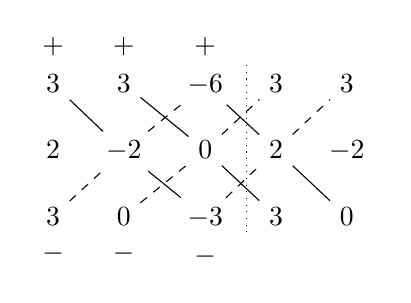
\begin{tikzpicture}
              \matrix [%
                matrix of math nodes,
                column sep=1em,
                row sep=1em
              ] (sarrus) {%
                3 & 3  & -6 & 3 & 3  \\
                2 & -2 & 0  & 2 & -2 \\
                3 & 0  & -3 & 3 & 0  \\
              };

              \path ($(sarrus-1-3.north east)+(0.5em,0)$) edge[dotted] ($(sarrus-3-3.south east)+(0.5em,0)$)
              (sarrus-1-1)                          edge         (sarrus-2-2)
              (sarrus-2-2)                          edge         (sarrus-3-3)
              (sarrus-1-2)                          edge         (sarrus-2-3)
              (sarrus-2-3)                          edge         (sarrus-3-4)
              (sarrus-1-3)                          edge         (sarrus-2-4)
              (sarrus-2-4)                          edge         (sarrus-3-5)
              (sarrus-3-1)                          edge[dashed] (sarrus-2-2)
              (sarrus-2-2)                          edge[dashed] (sarrus-1-3)
              (sarrus-3-2)                          edge[dashed] (sarrus-2-3)
              (sarrus-2-3)                          edge[dashed] (sarrus-1-4)
              (sarrus-3-3)                          edge[dashed] (sarrus-2-4)
              (sarrus-2-4)                          edge[dashed] (sarrus-1-5);

              \foreach \c in {1,2,3} {\node[anchor=south] at (sarrus-1-\c.north) {$+$};};
              \foreach \c in {1,2,3} {\node[anchor=north] at (sarrus-3-\c.south) {$-$};};
            \end{tikzpicture}
          \end{center}
          \sol{}
          \begin{flalign*}
            \vm{
            3 & 3                          & -6 \\
            2 & -2                         & 0  \\
            3 & 0                          & -3
            } & = 18 + 0 + 0 - 36 - 0 + 18      \\
              & = 0
          \end{flalign*}

    \item $\vm{
              5 & 7 & 1\\
              -3 & 6 & 9\\
              4 & 7 & 3
            }$
          \begin{center}
            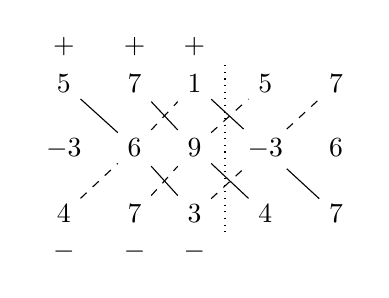
\begin{tikzpicture}
              \matrix [%
                matrix of math nodes,
                column sep=1em,
                row sep=1em
              ] (sarrus) {%
                5  & 7 & 1 & 5  & 7 \\
                -3 & 6 & 9 & -3 & 6 \\
                4  & 7 & 3 & 4  & 7 \\
              };

              \path ($(sarrus-1-3.north east)+(0.5em,0)$) edge[dotted] ($(sarrus-3-3.south east)+(0.5em,0)$)
              (sarrus-1-1)                          edge         (sarrus-2-2)
              (sarrus-2-2)                          edge         (sarrus-3-3)
              (sarrus-1-2)                          edge         (sarrus-2-3)
              (sarrus-2-3)                          edge         (sarrus-3-4)
              (sarrus-1-3)                          edge         (sarrus-2-4)
              (sarrus-2-4)                          edge         (sarrus-3-5)
              (sarrus-3-1)                          edge[dashed] (sarrus-2-2)
              (sarrus-2-2)                          edge[dashed] (sarrus-1-3)
              (sarrus-3-2)                          edge[dashed] (sarrus-2-3)
              (sarrus-2-3)                          edge[dashed] (sarrus-1-4)
              (sarrus-3-3)                          edge[dashed] (sarrus-2-4)
              (sarrus-2-4)                          edge[dashed] (sarrus-1-5);

              \foreach \c in {1,2,3} {\node[anchor=south] at (sarrus-1-\c.north) {$+$};};
              \foreach \c in {1,2,3} {\node[anchor=north] at (sarrus-3-\c.south) {$-$};};
            \end{tikzpicture}
          \end{center}
          \sol{}
          \begin{flalign*}
            \vm{
            5  & 7                               & 1 \\
            -3 & 6                               & 9 \\
            4  & 7                               & 3
            }  & = 90 + 252 - 21 - 24 - 315 + 63     \\
               & = 45
          \end{flalign*}

    \item $\vm{
              -2 & 7 & -4\\
              3 & -5 & 2\\
              -1 & 0 & -3
            }$
          \begin{center}
            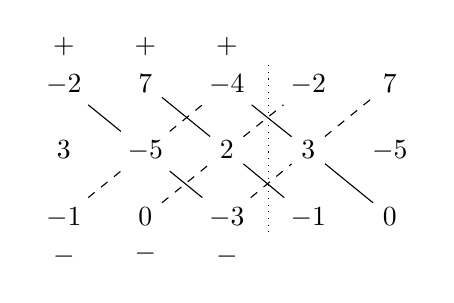
\begin{tikzpicture}
              \matrix [%
                matrix of math nodes,
                column sep=1em,
                row sep=1em
              ] (sarrus) {%
                -2 & 7  & -4 & -2 & 7  \\
                3  & -5 & 2  & 3  & -5 \\
                -1 & 0  & -3 & -1 & 0  \\
              };

              \path ($(sarrus-1-3.north east)+(0.5em,0)$) edge[dotted] ($(sarrus-3-3.south east)+(0.5em,0)$)
              (sarrus-1-1)                          edge         (sarrus-2-2)
              (sarrus-2-2)                          edge         (sarrus-3-3)
              (sarrus-1-2)                          edge         (sarrus-2-3)
              (sarrus-2-3)                          edge         (sarrus-3-4)
              (sarrus-1-3)                          edge         (sarrus-2-4)
              (sarrus-2-4)                          edge         (sarrus-3-5)
              (sarrus-3-1)                          edge[dashed] (sarrus-2-2)
              (sarrus-2-2)                          edge[dashed] (sarrus-1-3)
              (sarrus-3-2)                          edge[dashed] (sarrus-2-3)
              (sarrus-2-3)                          edge[dashed] (sarrus-1-4)
              (sarrus-3-3)                          edge[dashed] (sarrus-2-4)
              (sarrus-2-4)                          edge[dashed] (sarrus-1-5);

              \foreach \c in {1,2,3} {\node[anchor=south] at (sarrus-1-\c.north) {$+$};};
              \foreach \c in {1,2,3} {\node[anchor=north] at (sarrus-3-\c.south) {$-$};};
            \end{tikzpicture}
          \end{center}
          \sol{}
          \begin{flalign*}
            \vm{
            -2 & 7                            & -4 \\
            3  & -5                           & 2  \\
            -1 & 0                            & -3
            }  & = -30 - 14 - 0 + 20 + 0 + 63      \\
               & = -39
          \end{flalign*}

    \item $\vm{
              1 & 0 & -1\\
              3 & -2 & 5\\
              -1 & 1 & 3
            }$
          \sol{}
          \begin{flalign*}
            \vm{
            1  & 0                   & -1 \\
            3  & -2                  & 5  \\
            -1 & 1                   & 3
            }  & = \vm{
            -2 & 5                        \\
            1  & 3
            } -3 \vm{
            0  & -1                       \\
            1  & 3
            } - \vm{
            0  & -1                       \\
            -2 & 5
            }                             \\
               & = -11 - 3 + 2 = -12
          \end{flalign*}

    \item $\vm{
              2 & 6 & 4\\
              1 & 3 & 1\\
              -2 & -6 & 5
            }$
          \sol{}
          \begin{flalign*}
            \vm{
            2  & 6                                              & 4 \\
            1  & 3                                              & 1 \\
            -2 & -6                                             & 5
            }  & = 3\vm{
            2  & 2                                              & 4 \\
            1  & 1                                              & 1 \\
            -2 & -2                                             & 5
            }  &                                                    \\
               & = 0\ \ \ \ \ \text{(col 1 and 2 are the same)}     \\
          \end{flalign*}

    \item $\vm{
              10 & 8 & -2\\
              15 & 16 & -3\\
              -5 & -4 & 1
            }$
          \sol{}
          \begin{flalign*}
            \vm{
            10 & 8                                              & -2 \\
            15 & 16                                             & -3 \\
            -5 & -4                                             & 1
            }  & = -5\vm{
            2  & 8                                              & 2  \\
            3  & 16                                             & 3  \\
            -1 & -4                                             & -1
            }                                                        \\
               & = 0\ \ \ \ \ \text{(col 1 and 3 are the same)}
          \end{flalign*}

  \end{enumerate}

  \noindent Using the identities of determinant, prove the following equations (Question 23
  to 24):

  \begin{enumerate}[wide, labelwidth=!, labelindent=0pt]
    \setcounter{enumi}{22}

    \item $\vm{
              bc & 1 & bc(b+c)\\
              ca & 1 & ca(c+a)\\
              ab & 1 & ab(a+b)
            } = 0$
          \prooff{}
          \begin{flalign*}
               & \vm{
            bc & 1                              & bc(b+c)   \\
            ca & 1                              & ca(c+a)   \\
            ab & 1                              & ab(a+b)
            }                                               \\
               & = a^2b^2c^2\vm{
            1  & \frac{1}{bc}                   & b+c       \\
            1  & \frac{1}{ca}                   & c+a       \\
            1  & \frac{1}{ab}                   & a+b
            }                                               \\
               & = a^2b^2c^2\vm{
            1  & \frac{1}{bc}                   & -a        \\
            1  & \frac{1}{ca}                   & -b        \\
            1  & \frac{1}{ab}                   & -c
            }  & C_3 \rightarrow C_3+(a+b+c)C_1             \\
               & = a^2b^2c^2\vm{
            1  & a                              & -a        \\
            1  & b                              & -b        \\
            1  & c                              & -c
            }  & C_2 \rightarrow C_2 + abcC_1               \\
               & = -a^2b^2c^2\vm{
            1  & a                              & a         \\
            1  & b                              & b         \\
            1  & c                              & c
            }                                               \\
               & = 0                            & C_2 = C_3
          \end{flalign*}

    \item $\vm{
              a & 1 & a^2(b+c)\\
              b & 1 & b^2(c+a)\\
              c & 1 & c^2(a+b)
            } = 0$
          \prooff{}
          \begin{flalign*}
                  & \vm{
            a     & 1                                                     & a^2(b+c)            \\
            b     & 1                                                     & b^2(c+a)            \\
            c     & 1                                                     & c^2(a+b)
            }                                                                                   \\
                  & = \vm {
            a     & 1                                                     & a^2(b+c)            \\
            b - a & 0                                                     & b^2(c+a) - a^2(b+c) \\
            c - a & 0                                                     & c^2(a+b) - a^2(b+c)
            }                                                                                   \\
                  & R_2 \rightarrow R_2 - R_1,\ R_3 \rightarrow R_3 - R_1                       \\
                  & = \vm {
            b-a   & b^2(c+a) - a^2(b+c)                                                         \\
            c-a   & c^2(a+b) - a^2(b+c)
            }                                                                                   \\
                  & = (b-a)[c^2(a+b) - a^2(b+c)]                                                \\
                  & \ \ \ \ - (c-a)[b^2(c+a) - a^2(b+c)]                                        \\
                  & = c^2(b-a)(b+a) - a^2(b+c)(c-a)                                             \\
                  & \ \ \ \ - b^2(c-a)(c+a) + a^2(b+c)(c-a)                                     \\
                  & = c^2(b^2-a^2) - b^2(c^2-a^2)                                               \\
                  & = b^2c^2 - a^2c^2 - b^2c^2 + a^2c^2                                         \\
                  & = 0
          \end{flalign*}

  \end{enumerate}

  Find the value of $x$ in the following expressions (Question 25 to 26):

  \begin{enumerate}[wide, labelwidth=!, labelindent=0pt]
    \setcounter{enumi}{24}

    \item $\vm{
              2x & 3 & x+5\\
              -3 & 2 & 1\\
              2 & 1 & 0
            } = 5x - 1$
          \sol{}
          \begin{flalign*}
            \vm{
            2x                 & 3        & x+5 \\
            -3                 & 2        & 1   \\
            2                  & 1        & 0
            }                  & = 5x - 1       \\
            x+5\vm{
            -3                 & 2              \\
            2                  & 1
            } - \vm{
            2x                 & 3              \\
            2                  & 1
            }                  & = 5x - 1       \\
            -7(x+5) - (2x - 6) & = 5x - 1       \\
            -7x - 35 -2x + 6   & = 5x - 1       \\
            -14x               & = 28           \\
            x                  & = -2
          \end{flalign*}

    \item $\vm{
              x+3 & 1 & 0\\
              x & 3 & 0\\
              1 & 0 & -x-2
            } = x + 6$
          \sol{}
          \begin{flalign*}
            \vm{
            x+3             & 1                       & 0    \\
            x               & 3                       & 0    \\
            1               & 0                       & -x-2
            }               & = x + 6                        \\
            -x-2\vm{
            x+3             & 1                              \\
            x               & 3
            }               & = x + 6                        \\
            -(x+2)(3x+9-x)  & = x + 6                        \\
            (x+2)(2x+9)     & = -x-6                         \\
            2x^2 + 13x + 18 & = -x-6                         \\
            2x^2 + 14x + 24 & = 0                            \\
            x^2 + 7x + 12   & = 0                            \\
            (x+4)(x+3)      & = 0                            \\
            x               & = -4 \text{ or } x = -3
          \end{flalign*}

  \end{enumerate}

  \begin{enumerate}[wide, labelwidth=!, labelindent=0pt]
    \setcounter{enumi}{26}

    \item Given an identity matrix $I = \m{ 1 & 0\\ 0 & 1 }$. Let $J = \m{ 0 & 1\\ -1 & 0
            }$, ${(2I+J)}^{-1} = rI + sJ$, find the value of $r$ and $s$. \sol{}
          \begin{flalign*}
            {(2I+J)}^{-1}   & = {\left[2\m{
            1               & 0                                \\
            0               & 1
            } + \m{
            0               & 1                                \\
            -1              & 0
            }\right]}^{-1}                                     \\
                            & = {\left[\m{
            2               & 0                                \\
            0               & 2
            } + \m{
            0               & 1                                \\
            -1              & 0
            }\right]}^{-1}                                     \\
                            & = \m{
            2               & 1                                \\
            -1              & 2
            }^{-1}                                             \\
                            & = \frac{1}{5}\m{
            2               & -1                               \\
            1               & 2
            }                                                  \\
                            & = \m{
            \frac{2}{5}     & -\frac{1}{5}                     \\
            \frac{1}{5}     & \frac{2}{5}
            }                                                  \\
            rI + sJ         & = r\m{
            1               & 0                                \\
            0               & 1
            } + s\m{
            0               & 1                                \\
            -1              & 0
            }                                                  \\
                            & = \m{
            r               & 0                                \\
            0               & r
            } + \m{
            0               & s                                \\
            -s              & 0
            }                                                  \\
                            & = \m{
            r               & s                                \\
            -s              & r
            }                                                  \\
            {(2I + J)}^{-1} & = rI + sJ                        \\
            \m{
            \frac{2}{5}     & -\frac{1}{5}                     \\
            \frac{1}{5}     & \frac{2}{5}
            }               & = \m{
            r               & s                                \\
            -s              & r
            }                                                  \\
            \therefore\ r   & = \frac{2}{5},\ s = -\frac{1}{5}
          \end{flalign*}

  \end{enumerate}

  \noindent Find the value of $a$ in the following matrices if they are non-inversible (Question 28 to 31):

  \begin{enumerate}[wide, labelwidth=!, labelindent=0pt]
    \setcounter{enumi}{27}

    \item $\m{
              3 & a\\
              -2 & 6
            }$
          \sol{}
          \begin{flalign*}
            \vm{
            3       & a     \\
            -2      & 6
            }       & = 0   \\
            18 + 2a & = 0   \\
            2a      & = -18 \\
            a       & = -9
          \end{flalign*}

    \item $\m{
              5a + 2 & 4\\
              6 & a
            }$
          \sol{}
          \begin{flalign*}
            \vm{
            5a + 2                            & 4              \\
            6                                 & a
            }                                 & = 0            \\
            5a^2 + 2a - 24                    & = 0            \\
            (x-2)(5x + 12)                    & = 0            \\
            x               = 2 \text{ or } x & = \frac{12}{5}
          \end{flalign*}

    \item $\m{
              -7 & a & 3\\
              2 & -3 & 1\\
              0 & -a & 4
            }$
          \sol{}
          \begin{flalign*}
            \vm{
            -7                       & a    & 3 \\
            2                        & -3   & 1 \\
            0                        & -a   & 4
            }                        & = 0      \\
            -7\vm{
            -3                       & 1        \\
            -a                       & 4
            } - 2\vm{
            a                        & 3        \\
            -a                       & 4
            }                        & =0       \\
            -7(-12 + a) - 2(4a + 3a) & = 0      \\
            84 - 7a - 14a            & = 0      \\
            21a                      & = 84     \\
            a                        & = 4
          \end{flalign*}

    \item $\m{
              a & -1 & 0\\
              4 & 0 & -2\\
              a+4 & a & -8
            }$
          \sol{}
          \begin{flalign*}
            \vm{
            a                  & -1                     & 0  \\
            4                  & 0                      & -2 \\
            a+4                & a                      & -8
            }                  & = 0                         \\
            a\vm{
            0                  & -2                          \\
            a                  & -8
            } + \vm {
            4                  & -2                          \\
            a+4                & -8
            }                                                \\
            2a^2 - 32 + 2a + 8 & = 0                         \\
            2a^2 + 2a - 24     & = 0                         \\
            a^2 + a - 12       & = 0                         \\
            (a+4)(a-3)         & = 0                         \\
            a                  & = -4 \text{ or } a = 3
          \end{flalign*}

  \end{enumerate}

  \noindent Find the inverse of the following matrices (Question 32 to 37):

  \begin{enumerate}[wide, labelwidth=!, labelindent=0pt]
    \setcounter{enumi}{31}

    \item $\m{
              2 & 5\\
              2 & 3
            }$
          \sol{}
          \begin{flalign*}
            \m{
            2            & 5                 \\
            2            & 3
            }^{-1}       & = -\frac{1}{4}\m{
            3            & -5                \\
            -2           & 2
            }                                \\
                         & = \m{
            -\frac{3}{4} & \frac{5}{4}       \\
            \frac{1}{2}  & -\frac{1}{2}
            }
          \end{flalign*}

    \item $\m{
              -2 & -1 \\
              4 & 6
            }$
          \sol{}
          \begin{flalign*}
            \m{
            -2           & -1                \\
            4            & 6
            }^{-1}       & = -\frac{1}{8}\m{
            6            & 1                 \\
            -4           & -2
            }                                \\
                         & = \m{
            -\frac{3}{8} & -\frac{1}{8}      \\
            \frac{1}{2}  & \frac{1}{4}
            }
          \end{flalign*}

    \item $\m{
              1 & 0 & 3\\
              3 & 1 & 9\\
              -2 & 2 & -4
            }$
          \sol{}
          \begin{flalign*}
                & \vm{
            1   & 0                      & 3            \\
            3   & 1                      & 9            \\
            -2  & 2                      & -4
            }  = 2                                      \\
                & \operatorname{adj} \m{
            1   & 0                      & 3            \\
            3   & 1                      & 9            \\
            -2  & 2                      & -4
            }                                           \\
                & = \m{
            \vm{
            1   & 9                                     \\
            2   & -4
            }   & -\vm{
            3   & 9                                     \\
            -2  & -4
            }   & \vm{
            3   & 1                                     \\
            -2  & 2
            }                                           \\
            -\vm{
            0   & 3                                     \\
            2   & -4
            }   & \vm{
            1   & 3                                     \\
            -2  & -4
            }   & -\vm{
            1   & 0                                     \\
            -2  & 2
            }                                           \\
            \vm{
            0   & 3                                     \\
            1   & 9                                     \\
            }   & -\vm{
            1   & 3                                     \\
            3   & 9
            }   & \vm{
            1   & 0                                     \\
            3   & 1
            }
            }'                                          \\
                & =\m{
            -22 & -6                     & 8            \\
            6   & 2                      & -2           \\
            -3  & 0                      & 1
            }'                                          \\
                & = \m{
            -22 & 6                      & -3           \\
            -6  & 2                      & 0            \\
            8   & -2                     & 1
            }'                                          \\
                & \therefore\ \m{
            1   & 0                      & 3            \\
            3   & 1                      & 9            \\
            -2  & 2                      & -4
            }^{-1}                                      \\
                & = \frac{1}{2}\m{
            -22 & 6                      & -3           \\
            -6  & 2                      & 0            \\
            8   & -2                     & 1
            }                                           \\
                & = \m{
            -11 & 3                      & -\frac{3}{2} \\
            -3  & 1                      & 0            \\
            4   & -1                     & \frac{1}{2}
            }
          \end{flalign*}

    \item $\m{
              1 & 2 & -3\\
              2 & 1 & -4\\
              -2 & 5 & 1
            }$
          \sol{}
          \begin{flalign*}
                & \vm{
            1   & 2                      & -3           \\
            2   & 1                      & -4           \\
            -2  & 5                      & 1
            }  = -3                                     \\
                & \operatorname{adj} \m{
            1   & 2                      & -3           \\
            2   & 1                      & -4           \\
            -2  & 5                      & 1
            }                                           \\
                & = \m{
            \vm{
            1   & -4                                    \\
            5   & 1
            }   & -\vm{
            2   & -4                                    \\
            -2  & 1
            }   & \vm{
            2   & 1                                     \\
            -2  & 5
            }                                           \\
            -\vm{
            2   & -3                                    \\
            5   & 1
            }   & \vm{
            1   & -3                                    \\
            -2  & 1
            }   & -\vm{
            1   & 2                                     \\
            -2  & 5
            }                                           \\
            \vm{
            2   & -3                                    \\
            1   & -4                                    \\
            }   & -\vm{
            1   & -3                                    \\
            2   & -4
            }   & \vm{
            1   & 2                                     \\
            2   & 1
            }
            }'                                          \\
                & = \m{
            21  & 6                      & 12           \\
            -17 & -5                     & -9           \\
            -5  & -2                     & -3
            }'                                          \\
                & = \m{
            21  & -17                    & -5           \\
            6   & -5                     & -2           \\
            12  & -9                     & -3
            }'                                          \\
                & \therefore\ \m{
            1   & 2                      & -3           \\
            2   & 1                      & -4           \\
            -2  & 5                      & 1
            }^{-1}                                      \\
                & = -\frac{1}{3}\m{
            21  & -17                    & -5           \\
            6   & -5                     & -2           \\
            12  & -9                     & -3
            }                                           \\
                & = \m{
            -7  & -\frac{17}{3}          & -\frac{5}{3} \\
            -2  & -\frac{5}{3}           & -\frac{2}{3} \\
            -4  & 3                      & 1
            }
          \end{flalign*}

    \item $\m{
              4 & 1 & 0\\
              0 & -2 & 3\\
              0 & -4 & 4
            }$
          \sol{}
          \begin{flalign*}
                        & \vm{
            4           & 1                      & 0            \\
            0           & -2                     & 3            \\
            0           & -4                     & 4
            }  = 16                                             \\
                        & \operatorname{adj} \m{
            4           & 1                      & 0            \\
            0           & -2                     & 3            \\
            0           & -4                     & 4
            }                                                   \\
                        & = \m{
            \vm{
            -2          & 3                                     \\
            -4          & 4
            }           & -\vm{
            0           & 3                                     \\
            0           & 4
            }           & \vm{
            0           & -2                                    \\
            0           & -4
            }                                                   \\
            -\vm{
            1           & 0                                     \\
            -4          & 4
            }           & \vm{
            4           & 0                                     \\
            0           & 4
            }           & -\vm{
            4           & 1                                     \\
            0           & -4
            }                                                   \\
            \vm{
            1           & 0                                     \\
            -2          & 3
            }           & -\vm{
            4           & 0                                     \\
            0           & 3
            }           & \vm{
            4           & 1                                     \\
            0           & -2
            }
            }'                                                  \\
                        & = \m{
            4           & 0                      & 0            \\
            -4          & 16                     & 16           \\
            3           & -12                    & -8
            }'                                                  \\
                        & = \m{
            4           & -4                     & 0            \\
            0           & 16                     & -12          \\
            9           & 16                     & -8
            }                                                   \\
                        & \therefore\ \m{
            4           & 1                      & 0            \\
            0           & -2                     & 3            \\
            0           & -4                     & 4
            }^{-1}                                              \\
                        & = \frac{1}{16}\m{
            4           & -4                     & 3            \\
            0           & 16                     & -12          \\
            0           & 16                     & -8
            }                                                   \\
                        & = \m{
            \frac{1}{4} & -\frac{1}{4}           & \frac{3}{16} \\
            0           & 1                      & -\frac{3}{4} \\
            0           & 1                      & -\frac{1}{2}
            }
          \end{flalign*}

    \item $\m{
              3 & 2 & 4\\
              -1 & -3 & 0\\
              1 & 0 & 3
            }$
          \sol{}
          \begin{flalign*}
                         & \vm{
            3            & 2                      & 4            \\
            -1           & -3                     & 0            \\
            1            & 0                      & 3
            }  = -9                                              \\
                         & \operatorname{adj} \m{
            3            & 2                      & 4            \\
            -1           & -3                     & 0            \\
            1            & 0                      & 3
            }                                                    \\
                         & = \m{
            \vm{
            -3           & 0                                     \\
            0            & 3
            }            & -\vm{
            -1           & 0                                     \\
            1            & 3
            }            & \vm{
            -1           & -3                                    \\
            1            & 0
            }                                                    \\
            -\vm{
            2            & 4                                     \\
            0            & 3
            }            & \vm{
            3            & 4                                     \\
            1            & 3
            }            & -\vm{
            3            & 2                                     \\
            1            & 0
            }                                                    \\
            \vm{
            2            & 4                                     \\
            -3           & 0
            }            & -\vm{
            3            & 4                                     \\
            -1           & 0
            }            & \vm{
            3            & 2                                     \\
            -1           & -3
            }
            }'                                                   \\
                         & = \m{
            -9           & 3                      & 3            \\
            -6           & 5                      & 2            \\
            12           & -4                     & -7
            }'                                                   \\
                         & = \m{
            -9           & -6                     & 12           \\
            3            & 5                      & -4           \\
            3            & 2                      & -7
            }                                                    \\
                         & \therefore\ \m{
            3            & 2                      & 4            \\
            -1           & -3                     & 0            \\
            1            & 0                      & 3
            }                                                    \\
                         & = \frac{1}{-9}\m{
            -9           & -6                     & 12           \\
            3            & 5                      & -4           \\
            3            & 2                      & -7
            }                                                    \\
                         & = \m{
            -1           & \frac{2}{3}            & -\frac{4}{3} \\
            -\frac{1}{3} & -\frac{5}{9}           & \frac{4}{9}  \\
            -\frac{1}{3} & -\frac{2}{9}           & \frac{7}{9}
            }
          \end{flalign*}

  \end{enumerate}

  \noindent Solve the following system of equations using the method of Gauss elimination (Question 38 to 41):

  \begin{enumerate}[wide, labelwidth=!, labelindent=0pt]
    \setcounter{enumi}{37}

    \item $\begin{cases}
              2x - y + 4z = 5   \\
              2x + 3y - 4z = -7 \\
              x + y + z = 2
            \end{cases}$
          \sol{}
          \begin{flalign*}
                                                                               & \begin{amatrix}{3}
                                                                                   2 & -1 & 4 & 5\\
                                                                                   2 & 3 & -4 & -7\\
                                                                                   1 & 1 & 1 & 2
                                                                                 \end{amatrix}    \\
            \xrightarrow[R_1 \rightarrow R_1 + R_3]{R_2 \rightarrow R_2 + R_1} & \begin{amatrix}{3}
                                                                                   3 & 0 & 5 & 7\\
                                                                                   4 & 2 & 0 & -2\\
                                                                                   1 & 1 & 1 & 2
                                                                                 \end{amatrix}    \\
            \xrightarrow{R_2 \rightarrow \frac{1}{2}R_2}                       & \begin{amatrix}{3}
                                                                                   3 & 0 & 5 & 7\\
                                                                                   2 & 1 & 0 & -1\\
                                                                                   1 & 1 & 1 & 2
                                                                                 \end{amatrix}    \\
            \xrightarrow{R_3 \rightarrow R_3 - R_2}                            & \begin{amatrix}{3}
                                                                                   3 & 0 & 5 & 7\\
                                                                                   2 & 1 & 0 & -1\\
                                                                                   -1 & 0 & 1 & 3
                                                                                 \end{amatrix}    \\
            \xrightarrow{R_1 \rightarrow R_1 + 3R_3}                           & \begin{amatrix}{3}
                                                                                   0 & 0 & 8 & 16\\
                                                                                   2 & 1 & 0 & -1\\
                                                                                   -1 & 0 & 1 & 3
                                                                                 \end{amatrix}    \\
            \xrightarrow{R_1 \rightarrow \frac{1}{8}R_1}                       & \begin{amatrix}{3}
                                                                                   0 & 0 & 1 & 2\\
                                                                                   2 & 1 & 0 & -1\\
                                                                                   -1 & 0 & 1 & 3
                                                                                 \end{amatrix}    \\
            \xrightarrow{R_3 \rightarrow R_3 - R_1}                            & \begin{amatrix}{3}
                                                                                   0 & 0 & 1 & 2\\
                                                                                   2 & 1 & 0 & -1\\
                                                                                   -1 & 0 & 0 & 1
                                                                                 \end{amatrix}    \\
            \xrightarrow[R_3 \rightarrow -R3]{R_2 \rightarrow R_2 + 2R_3}      & \begin{amatrix}{3}
                                                                                   0 & 0 & 1 & 2\\
                                                                                   0 & 1 & 0 & 1\\
                                                                                   1 & 0 & 0 & -1
                                                                                 \end{amatrix}    \\
            \xrightarrow{R_1 \leftrightarrow R_2}                              & \begin{amatrix}{3}
                                                                                   1 & 0 & 0 & -1\\
                                                                                   0 & 1 & 0 & 1\\
                                                                                   0 & 0 & 1 & 2\\
                                                                                 \end{amatrix}    \\
            \therefore\ x                                                      & = -1,\ y = 1,\ z = 2
          \end{flalign*}

    \item $\begin{cases}
              x - 2y - 3z = -4 \\
              3x + y - 4z = -5 \\
              2x + 4y - z = -5
            \end{cases}$
          \sol{}
          \begin{flalign*}
                                                                                  & \begin{amatrix}{3}
                                                                                      1 & -2 & -3 & -4\\
                                                                                      3 & 1 & -4 & -5\\
                                                                                      2 & 4 & -1 & -5
                                                                                    \end{amatrix}    \\
            \xrightarrow[R_2 \rightarrow R_2 - 3R_1]{R_3 \rightarrow R_3 - 2R_1}  & \begin{amatrix}{3}
                                                                                      1 & -2 & -3 & -4\\
                                                                                      0 & 7 & 5 & 7\\
                                                                                      0 & 8 & 5 & 3
                                                                                    \end{amatrix}    \\
            \xrightarrow{R_3 \rightarrow R_3 - R_1}                               & = \begin{amatrix}{3}
                                                                                        1 & -2 & -3 & -4\\
                                                                                        0 & 7 & 5 & 7\\
                                                                                        0 & 1 & 0 & -4
                                                                                      \end{amatrix}  \\
            \xrightarrow[R_2 \rightarrow R_2 - 7R_3]{R_1 \rightarrow R_1 + 2R_3}  & = \begin{amatrix}{3}
                                                                                        1 & 0 & -3 & -12\\
                                                                                        0 & 0 & 5 & 35\\
                                                                                        0 & 1 & 0 & -4
                                                                                      \end{amatrix}  \\
            \xrightarrow[R_2 \leftrightarrow R_3]{R_2 \rightarrow \frac{1}{5}R_2} & = \begin{amatrix}{3}
                                                                                        1 & 0 & -3 & -12\\
                                                                                        0 & 1 & 0 & -4\\
                                                                                        0 & 0 & 1 & 7
                                                                                      \end{amatrix}  \\
            \xrightarrow{R_1 \rightarrow R_1 + 3R_2}                              & = \begin{amatrix}{3}
                                                                                        1 & 0 & 0 & 9\\
                                                                                        0 & 1 & 0 & -4\\
                                                                                        0 & 0 & 1 & 7
                                                                                      \end{amatrix}  \\
            \therefore\ x                                                         & = 9,\ y = -4,\ z = 7
          \end{flalign*}

    \item $\begin{cases}
              x - 2y - z = 3  \\
              4x - y + 2z = 1 \\
              x + 3y = 5
            \end{cases}$
          \sol{}
          \begin{flalign*}
                                                                                    & \begin{amatrix}{3}
                                                                                        1 & -2 & -1 & 3\\
                                                                                        4 & -1 & 2 & 1\\
                                                                                        1 & 3 & 0 & 5
                                                                                      \end{amatrix}    \\
            \xrightarrow[R_2 \rightarrow R_2 - 4R_3]{R_1 \rightarrow R_1 - R_3}     & \begin{amatrix}{3}
                                                                                        0 & -5 & -1 & -2\\
                                                                                        0 & -13 & 2 & -19\\
                                                                                        1 & 3 & 0 & 5
                                                                                      \end{amatrix}    \\
            \xrightarrow{R_2 \rightarrow R_2 + 2R_1}                                & \begin{amatrix}{3}
                                                                                        0 & -5 & -1 & -2\\
                                                                                        0 & -23 & 0 & -23\\
                                                                                        1 & 3 & 0 & 5
                                                                                      \end{amatrix}    \\
            \xrightarrow[R_1 \leftrightarrow R_3]{R_2 \rightarrow -\frac{1}{23}R_2} & \begin{amatrix}{3}
                                                                                        1 & 3 & 0 & 5\\
                                                                                        0 & 1 & 0 & 1\\
                                                                                        0 & -5 & -1 & -2
                                                                                      \end{amatrix}    \\
            \xrightarrow[R_3 \rightarrow R_3 + 5R_2]{R_1 \rightarrow R_1 - 3R_2}    & \begin{amatrix}{3}
                                                                                        1 & 0 & 0 & 2\\
                                                                                        0 & 1 & 0 & 1\\
                                                                                        0 & 0 & 1 & -3
                                                                                      \end{amatrix}    \\
            \therefore\ x                                                           & = 2,\ y = 1,\ z = -3
          \end{flalign*}

    \item $\begin{cases}
              2x - y - z = 0   \\
              4x - 3y + 2z = 1 \\
              3x - 2y - 4z = -1
            \end{cases}$
          \sol{}
          \begin{flalign*}
                                                                               & \begin{amatrix}{3}
                                                                                   2 & -1 & -1 & 0\\
                                                                                   4 & -3 & 2 & 1\\
                                                                                   3 & -2 & -4 & -1
                                                                                 \end{amatrix}                                 \\
            \xrightarrow{R_2 \rightarrow R_2 - 2R_1}                           & \begin{amatrix}{3}
                                                                                   2 & -1 & -1 & 0\\
                                                                                   0 & -1 & 4 & 1\\
                                                                                   3 & -2 & -4 & -1
                                                                                 \end{amatrix}                                 \\
            \xrightarrow[R_1 \rightarrow R_1 - R_2]{R_3 \rightarrow R_3 + R_2} & \begin{amatrix}{3}
                                                                                   2 & 0 & -5 & -1\\
                                                                                   0 & -1 & 4 & 1\\
                                                                                   3 & -3 & 0 & 0
                                                                                 \end{amatrix}                                 \\
            \xrightarrow{R_3 \rightarrow \frac{1}{3}R_3}                       & \begin{amatrix}{3}
                                                                                   2 & 0 & -5 & -1\\
                                                                                   0 & -1 & 4 & 1\\
                                                                                   1 & -1 & 0 & 0
                                                                                 \end{amatrix}                                 \\
            \xrightarrow{R_2 \rightarrow R_2 - R_3}                            & \begin{amatrix}{3}
                                                                                   2 & 0 & -5 & -1\\
                                                                                   -1 & 0 & 4 & 1\\
                                                                                   1 & -1 & 0 & 0
                                                                                 \end{amatrix}                                 \\
            \xrightarrow{R_1 \rightarrow R_1 + 2R_2}                           & \begin{amatrix}{3}
                                                                                   0 & 0 & 3 & 1\\
                                                                                   -1 & 0 & 4 & 1\\
                                                                                   1 & -1 & 0 & 0
                                                                                 \end{amatrix}                                 \\
            \xrightarrow{R_1 \rightarrow \frac{1}{3}R_1}                       & \begin{amatrix}{3}
                                                                                   0 & 0 & 1 & \frac{1}{3}\\
                                                                                   -1 & 0 & 4 & 1\\
                                                                                   1 & -1 & 0 & 0
                                                                                 \end{amatrix}                            \\
            \xrightarrow[R_3 \leftrightarrow R_2]{R_2 \rightarrow R_2 - 4R_1}  & \begin{amatrix}{3}
                                                                                   1 & -1 & 0 & 0\\
                                                                                   -1 & 0 & 0 & -\frac{1}{3}\\
                                                                                   0 & 0 & 1 & \frac{1}{3}\\
                                                                                 \end{amatrix}                          \\
            \xrightarrow{R_2 \rightarrow -R_2}                                 & \begin{amatrix}{3}
                                                                                   1 & -1 & 0 & 0\\
                                                                                   1 & 0 & 0 & \frac{1}{3}\\
                                                                                   0 & 0 & 1 & \frac{1}{3}\\
                                                                                 \end{amatrix}                            \\
            \xrightarrow{R_1 \rightarrow R_1 - R_2}                            & \begin{amatrix}{3}
                                                                                   0 & -1 & 0 & -\frac{1}{3}\\
                                                                                   1 & 0 & 0 & \frac{1}{3}\\
                                                                                   0 & 0 & 1 & \frac{1}{3}\\
                                                                                 \end{amatrix}                          \\
            \xrightarrow{R_1 \rightarrow -R_1}                                 & \begin{amatrix}{3}
                                                                                   0 & 1 & 0 & \frac{1}{3}\\
                                                                                   1 & 0 & 0 & \frac{1}{3}\\
                                                                                   0 & 0 & 1 & \frac{1}{3}\\
                                                                                 \end{amatrix}                            \\
            \xrightarrow{R_1 \leftrightarrow R_2}                              & \begin{amatrix}{3}
                                                                                   1 & 0 & 0 & \frac{1}{3}\\
                                                                                   0 & 1 & 0 & \frac{1}{3}\\
                                                                                   0 & 0 & 1 & \frac{1}{3}\\
                                                                                 \end{amatrix}                            \\
            \therefore\ x                                                      & = \frac{1}{3},\ y = \frac{1}{3},\ z = \frac{1}{3}
          \end{flalign*}

  \end{enumerate}

  \noindent Solve the following system of equations using the Cramer's rule (Question 42 to 45):

  \begin{enumerate}[wide, labelwidth=!, labelindent=0pt]
    \setcounter{enumi}{41}

    \item $\begin{cases}
              x - 3y - 2z = 1  \\
              7x + 4y - 5z = 0 \\
              3x + 9y + z = -1
            \end{cases}$
          \sol{}
          \begin{flalign*}
            \Delta        & = \vm{
            1             & -3                                                                    & -2 \\
            7             & 4                                                                     & -5 \\
            3             & 9                                                                     & 1
            }         = 13                                                                             \\
            \Delta_x      & = \vm{
            1             & -3                                                                    & -2 \\
            0             & 4                                                                     & -5 \\
            -1            & 9                                                                     & 1
            }         = 26                                                                             \\
            \Delta_y      & = \vm{
            1             & 1                                                                     & -2 \\
            7             & 0                                                                     & -5 \\
            3             & -1                                                                    & 1
            }         = -13                                                                            \\
            \Delta_z      & = \vm{
            1             & -3                                                                    & 1  \\
            7             & 4                                                                     & 0  \\
            3             & 9                                                                     & -1
            }         = 26                                                                             \\
            \therefore\ x & = \frac{26}{13} = 2,\ y = \frac{-13}{13} = -1,\ z = \frac{26}{13} = 2
          \end{flalign*}

    \item $\begin{cases}
              x - 2y + 3z = 6   \\
              2x + 3y - 4z = 20 \\
              3x - 2y - 5z = 6
            \end{cases}$
          \sol{}
          \begin{flalign*}
            \Delta        & = \vm{
            1             & -2                                                                           & 3  \\
            2             & 3                                                                            & -4 \\
            3             & -2                                                                           & -5
            } = -58                                                                                           \\
            \Delta_x      & = \vm{
            6             & -2                                                                           & 3  \\
            20            & 3                                                                            & -4 \\
            6             & -2                                                                           & -5
            } = -464                                                                                          \\
            \Delta_y      & = \vm{
            1             & 6                                                                            & 3  \\
            2             & 20                                                                           & -4 \\
            3             & 6                                                                            & -5
            } = -232                                                                                          \\
            \Delta_z      & = \vm{
            1             & -2                                                                           & 6  \\
            2             & 3                                                                            & 20 \\
            3             & -2                                                                           & 6
            } = -116                                                                                          \\
            \therefore\ x & = \frac{-464}{-58} = 8,\ y = \frac{-232}{-58} = 4,\ z = \frac{-116}{-58} = 2
          \end{flalign*}

    \item $\begin{cases}
              2x - 2y - 4z + 3 = 0 \\
              2x + 3y + 4z - 2 = 0 \\
              7x + 3y - 2z - 2 = 0
            \end{cases}$
          \sol{}
          \begin{flalign*}
                          & \begin{cases}
                              2x - 2y - 4z = -3 \\
                              2x + 3y + 4z = 2  \\
                              7x + 3y - 2z = 2
                            \end{cases}                                                             \\
            \Delta        & = \vm{
            2             & -2                                                                                            & -4 \\
            2             & 3                                                                                             & 4  \\
            7             & 3                                                                                             & -2
            } = -40                                                                                                            \\
            \Delta_x      & = \vm{
            -3            & -2                                                                                            & -4 \\
            2             & 3                                                                                             & 4  \\
            2             & 3                                                                                             & -2
            } = 30                                                                                                             \\
            \Delta_y      & = \vm{
            2             & -3                                                                                            & -4 \\
            2             & 2                                                                                             & 4  \\
            7             & 2                                                                                             & -2
            } = -80                                                                                                            \\
            \Delta_z      & = \vm{
            2             & -2                                                                                            & -3 \\
            2             & 3                                                                                             & 2  \\
            7             & 3                                                                                             & 2
            } = 25                                                                                                             \\
            \therefore\ x & = \frac{30}{-40} = -\frac{3}{4},\ y = \frac{-80}{-40} = 2,\ z = \frac{25}{-40} = -\frac{5}{8}
          \end{flalign*}

    \item $\begin{cases}
              \frac{2}{x} - \frac{5}{y} + \frac{4}{z} = -3 \\
              \frac{4}{x} + \frac{1}{y} - \frac{2}{z} = 7  \\
              \frac{7}{x} - \frac{3}{z} = 4
            \end{cases}$
          \sol{}
          \begin{flalign*}
            \text{Let }   & a = \frac{1}{x},\ b = \frac{1}{y},\ c = \frac{1}{z}                                                    \\
                          & \begin{cases}
                              2a - 5b + 4c = -3 \\
                              4a + b - 2c = 7   \\
                              7a - 3c = 4
                            \end{cases}                                                                 \\
            \Delta        & = \vm{
            2             & -5                                                                                                & 4  \\
            4             & 1                                                                                                 & -2 \\
            7             & 0                                                                                                 & -3
            } = -24                                                                                                                \\
            \Delta_a      & = \vm{
            -3            & -5                                                                                                & 4  \\
            7             & 1                                                                                                 & -2 \\
            4             & 0                                                                                                 & -3
            } = -72                                                                                                                \\
            \Delta_b      & = \vm{
            2             & -3                                                                                                & 4  \\
            4             & 7                                                                                                 & -2 \\
            7             & 4                                                                                                 & -3
            } = -152                                                                                                               \\
            \Delta_c      & = \vm{
            2             & -5                                                                                                & -3 \\
            4             & 1                                                                                                 & 7  \\
            7             & 0                                                                                                 & 4
            } = -136                                                                                                               \\
            \therefore\ a & = \frac{-72}{-24} = 3,\ b = \frac{-152}{-24} = \frac{19}{3},\ c = \frac{-136}{-24} = \frac{17}{3}      \\
            \therefore\ x & = \frac{1}{3},\ y = \frac{3}{19},\ z = \frac{3}{17}
          \end{flalign*}

  \end{enumerate}

  \chapter{Inequalities and Linear Programming}

  \section{Inequalities and its Identities}

  \subsection*{Inequalities}

  An inequality is a relation which makes a non-equal comparison between two
  numbers or other mathematical expressions. For example:
  \begin{flalign*}
    11 > 10 \\
    x^2 + 5 < 6x
  \end{flalign*}

  \begin{itemize}
    \item $a < b$ means $a$ is lesser than $b$
    \item $a > b$ means $a$ is greater than $b$
    \item $a \leq b$ means $a$ is lesser than or equal to $b$
    \item $a \geq b$ means $a$ is greater than or equal to $b$
  \end{itemize}

  \noindent For any real number $a$ and $b$, the following are true:
  \begin{enumerate}
    \item If $a - b > 0$, then $a > b$
    \item If $a - b < 0$, then $a < b$
  \end{enumerate}
  That means, if we want to compare between two numbers, we just have to calculate their difference.

  \subsection{Practice 1}

  Compare the following algebraic expressions:

  \begin{enumerate}
    \item $(x+3)(x-1)$ and $(x+4)(x-2)$
          \sol{}
          \begin{flalign*}
                         & (x+3)(x-1) - (x+4)(x-2)         \\
                         & = x^2 + 2x - 3 - (x^2 + 2x - 8) \\
                         & = x^2 + 2x - 3 - x^2 - 2x + 8   \\
                         & = 5 > 0                         \\
            \therefore\  & (x+3)(x-1) > (x+4)(x-2)
          \end{flalign*}

    \item $(x+8)(x+10)$ and ${(x+9)}^2$
          \sol{}
          \begin{flalign*}
                         & (x+8)(x+10) - {(x+9)}^2             \\
                         & = x^2 + 18x + 80 - (x^2 + 18x + 81) \\
                         & = x^2 + 18x + 80 - x^2 - 18x - 81   \\
                         & = -1 < 0                            \\
            \therefore\  & (x+8)(x+10) < {(x+9)}^2
          \end{flalign*}

    \item $x^2 + 6x$ and $4x-2$
          \sol{}
          \begin{flalign*}
                         & x^2 + 6x - 4x + 2     \\
                         & = x^2 + 2x + 2        \\
                         & = {(x + 1)}^2 - 1 + 2 \\
                         & = {(x + 1)}^2 + 1     \\
            \because\    & {(x+1)}^2 > 0         \\
            \therefore\  & {(x+1)}^2 + 1 > 0     \\
            \therefore\  & x^2 + 6x > 4x - 2
          \end{flalign*}
  \end{enumerate}

  \subsection*{Identities of Inequalities}

  \setcounter{theorem}{0}
  \begin{theorem}
    If $a > b$, $b > c$, then $a > c$
  \end{theorem}
  \begin{theorem}
    If $a > b$ then $a + c > b + c$
  \end{theorem}
  \begin{theorem}
    If $a > b$, $c > d$, then $a + c > b + d$
  \end{theorem}
  \begin{theorem}
    If $a > b$, then:
    \begin{enumerate}
      \item When $c > 0$, $ac > bc$
      \item When $c = 0$, $ac = bc$
      \item When $c < 0$, $ac < bc$
    \end{enumerate}
  \end{theorem}

  \subsection{Practice 2}

  Given that $y < x < 0$, use inequality signs to complete the following
  statements:

  \begin{enumerate}
    \item $x+1$ and $y+1$
          \sol{}
          \begin{flalign*}
            \because\    & y < x     \\
            \therefore\  & y+1 < x+1
          \end{flalign*}

    \item $2y$ and $2x$
          \sol{}
          \begin{flalign*}
            \because\    & y < x,\ 2 > 0 \\
            \therefore\  & 2y < 2x
          \end{flalign*}

    \item $-x + 1$ and $-y + 2$
          \sol{}
          \begin{flalign*}
            \because\    & y < x           \\
            \therefore\  & -x < -y         \\
            \because\    & 1 < 2,\ -x < -y \\
            \therefore\  & -x + 1 < -y + 2
          \end{flalign*}

    \item $3x$ and $4y$
          \sol{}
          \begin{flalign*}
            \because\    & y < x                      \\
            \therefore\  & 3y < 3x       & \cdots (1) \\
            and,\        & y < 0         & \cdots (2) \\
            (1) + (2):   & \ 3y + y < 3x              \\
                         & \ 4y < 3x
          \end{flalign*}
  \end{enumerate}

  \subsection{Exercise 15.1}

  Compare the following algebraic expressions (Question 1 to 5):

  \begin{enumerate}[wide, labelwidth=!, labelindent=0pt]

    \item ${(x-4)}^2$ and $(x-6)(x-2)$
          \sol{}
          \begin{flalign*}
                         & {(x-4)}^2 - (x-6)(x-2)            \\
                         & = x^2 - 8x + 16 - (x^2 - 8x + 12) \\
                         & = x^2 - 8x + 16 - x^2 + 8x - 12   \\
                         & = 4 > 0                           \\
            \therefore\  & {(x-4)}^2 > (x-6)(x-2)
          \end{flalign*}

    \item $x^2 + 13$ and $4x$
          \sol{}
          \begin{flalign*}
                         & x^2 + 13 - 4x        \\
                         & = x^2 - 4x + 13      \\
                         & = {(x-2)}^2 - 4 + 13 \\
                         & = {(x-2)}^2 + 9      \\
            \because\    & {(x-2)}^2 > 0        \\
            \therefore\  & {(x-2)}^2 + 9 > 0    \\
            \therefore\  & x^2 + 13 > 4x
          \end{flalign*}
    \item $(x-1)(x^2 + x + 1)$ and $(x+1)(x^2 - x + 1)$
          \sol{}
          \begin{flalign*}
                         & (x-1)(x^2 + x + 1) - (x+1)(x^2 - x + 1) \\
                         & = x^3 - 1 - x^3 - 1                     \\
                         & = -2 < 0                                \\
            \therefore\  & (x-1)(x^2 + x + 1) < (x+1)(x^2 - x + 1)
          \end{flalign*}

    \item $(x^2 - x + 1)(x^2 + x + 1)$ and $x^4 + x^2 - 1$
          \sol{}
          \begin{flalign*}
                         & (x^2 - x + 1)(x^2 + x + 1) - x^4 - x^2 + 1                      & \\
                         & = x^4 + x^3 + x^2 - x^3 - x^2 - x + x^2 + x + 1 - x^4 - x^2 + 1 & \\
                         & = 2 > 0                                                         & \\
            \therefore\  & (x^2 - x + 1)(x^2 + x + 1) > x^4 + x^2 - 1
          \end{flalign*}

    \item $(1 - 2x)(1 + 2x)$ and ${(x^2 - 6)}^2$
          \sol{}
          \begin{flalign*}
                         & {(x^2 - 6)}^2 - (1 - 2x)(1 + 2x) \\
                         & = x^4 - 12x^2 + 36 - 1 + 4x^2    \\
                         & = x^4 - 8x^2 + 35                \\
                         & = {(x^2 - 4)}^2 - 16 + 35        \\
                         & = {(x^2 - 4)}^2 + 19             \\
            \because\    & {(x^2 - 4)}^2 > 0                \\
            \therefore\  & {(x^2 - 4)}^2 + 19 > 0           \\
            \therefore\  & {(x^2 - 6)}^2 > (1 - 2x)(1 + 2x) \\
          \end{flalign*}

    \item Given that $y < x < 0$, use inequality signs to complete the following:
          \begin{enumerate}

            \item $2x - 3$ and $2y - 5$
                  \sol{}
                  \begin{flalign*}
                    \because\    & y < x,\ 2 > 0     \\
                    \therefore\  & 2y < 2x           \\
                    \because\    & -3 > -5,\ 2x > 2y \\
                    \therefore\  & 2x - 3 > 2y - 5
                  \end{flalign*}

            \item $x^2$ and $y^2$
                  \sol{}
                  \begin{flalign*}
                    \because\    & y < x,\ x^2 > 0,\ y^2 > 0 \\
                    \therefore\  & y^2 < x^2
                  \end{flalign*}

          \end{enumerate}

  \end{enumerate}

  \section{Linear Inequalities}

  \subsection*{Solving Linear Inequalities}

  The general form of a linear inequality is $ax + b \leq c$, where $a \neq 0$.

  \subsection{Practice 3}

  Solve the following linear inequalities:

  \begin{enumerate}
    \item $2x > x + 9$
          \sol{}
          \begin{flalign*}
            2x & > x + 9 \\
            x  & > 9
          \end{flalign*}

    \item $11 - 2x \leq -7$
          \sol{}
          \begin{flalign*}
            11 - 2x & \leq -7  \\
            -2x     & \leq -18 \\
            2x      & \geq 18  \\
            x       & \geq 9
          \end{flalign*}

    \item $2(x + 2) \geq \frac{2}{3} + \frac{2x+3}{4}$
          \sol{}
          \begin{flalign*}
            2(x + 2) & \geq \frac{2}{3} + \frac{2x+3}{4} \\
            2x + 4   & \geq \frac{2}{3} + \frac{2x+3}{4} \\
            24x + 48 & \geq 8 + 6x + 9                   \\
            24x + 48 & \geq 17 + 6x                      \\
            18x      & \geq -31                          \\
            x        & \geq -\frac{31}{18}
          \end{flalign*}

    \item $2x - \frac{x}{3} + \frac{1}{3} < 3x - \frac{1}{2} + \frac{x}{6}$
          \sol{}
          \begin{flalign*}
            2x - \frac{x}{3} + \frac{1}{3} & < 3x - \frac{1}{2} + \frac{x}{6} \\
            12x - 2x + 2                   & < 18x - 3 + x                    \\
            10x + 2                        & < 19x - 3                        \\
            -9x                            & < -5                             \\
            x                              & > \frac{5}{9}
          \end{flalign*}

    \item $10 \leq x + 3 \leq 12$
          \sol{}
          \begin{flalign*}
            10 & \leq x + 3 \leq 12  \\
            7  & \leq x       \leq 9
          \end{flalign*}

    \item $-3 < 7 - 2x < 9$
          \sol{}
          \begin{flalign*}
            -3  & < 7 - 2x < 9 \\
            -10 & < -2x < 2    \\
            -2  & < 2x < 10    \\
            -1  & < x < 5
          \end{flalign*}
  \end{enumerate}

  \subsection{Practice 15.2a}

  Solve the following linear inequalities:

  \begin{enumerate}
    \item $4x - 3 > x + 9$
          \sol{}
          \begin{flalign*}
            4x - 3 & > x + 9 \\
            3x     & > 12    \\
            x      & > 4
          \end{flalign*}

    \item $-4x > 1 - x$
          \sol{}
          \begin{flalign*}
            -4x & > 1 - x \\
            -3x > 1       \\
            3x < -1       \\
            x < -\frac{1}{3}
          \end{flalign*}

    \item $3x + 20 \geq 34 - 4x$
          \sol{}
          \begin{flalign*}
            7x & \geq 14 \\
            7x & \geq 14 \\
          \end{flalign*}

    \item $5x + 8 \leq 6x - 7$
          \sol{}
          \begin{flalign*}
            5x + 8 & \leq 6x - 7 \\
            -x \leq -15          \\
            x \geq 15
          \end{flalign*}
    \item $1 \leq 6(x-7)$
          \sol{}
          \begin{flalign*}
            1  & \leq 6(x-7)       \\
            1  & \leq 6x - 42      \\
            6x & \geq 43           \\
            x  & \geq \frac{43}{6}
          \end{flalign*}
    \item $2(x+7) \leq 5x + 14$
          \sol{}
          \begin{flalign*}
            2(x+7)  & \leq 5x + 14 \\
            2x + 14 & \leq 5x + 14 \\
            -3x     & \leq 0       \\
            x       & \geq 0
          \end{flalign*}

    \item $\frac{x}{2} + \frac{2 - 3x}{5} > -\frac{7}{2} + \frac{x+1}{5}$
          \sol{}
          \begin{flalign*}
            \frac{x}{2} + \frac{2 - 3x}{5} & > -\frac{7}{2} + \frac{x+1}{5} \\
            5x + 4 - 6x                    & > -35 + 2x + 2                 \\
            -x + 4                         & > -33 + 2x                     \\
            -3x                            & > -37                          \\
            x                              & < \frac{37}{3}
          \end{flalign*}

    \item $-5 < 12 - x < -1$
          \sol{}
          \begin{flalign*}
            -5  & < 12 - x < -1 \\
            -17 & < -x < -13    \\
            13  & < x < 17
          \end{flalign*}

    \item $-\frac{3}{5} < \frac{x}{2} - \frac{1}{2} < \frac{2}{5}$
          \sol{}
          \begin{flalign*}
            -6           & < 5x - 5 < 4      \\
            -1           & < 5x < 9          \\
            -\frac{1}{5} & < x < \frac{9}{5}
          \end{flalign*}

    \item $-2 < \frac{2x}{3} + \frac{1}{2} \leq 4$
          \sol{}
          \begin{flalign*}
            -12           & < 4x + 3 \leq 24      \\
            -15           & < 4x \leq 21          \\
            -\frac{15}{4} & < x \leq \frac{21}{4}
          \end{flalign*}
  \end{enumerate}

\end{multicols}
\end{document}